\documentclass{book}
\usepackage{helvet} % Helvetica font
\renewcommand{\familydefault}{\sfdefault} % Set default font to Helvetica
\usepackage[most]{tcolorbox} % For colored boxes
\usepackage{xcolor} % For custom colors
\usepackage{titlesec} % For customizing chapter headings
\usepackage[margin=0.5in]{geometry} % Set smaller margins
\usepackage{hyperref}
\usepackage{verbatim}

% Define custom colors
\definecolor{definitioncolor}{RGB}{51, 155, 255}
\definecolor{theoremcolor}{RGB}{97, 232, 26}
\definecolor{ideacolor}{RGB}{253, 218, 13}
\definecolor{warningcolor}{RGB}{255, 87, 51}
\definecolor{examplecolor}{RGB}{66, 64, 227}

% Define tcolorbox styles for different types of content
\tcbset{
    commonbox/.style 2 args={
        enhanced,
        arc=0pt,
        boxrule=0pt,
        frame hidden,
        colback={#1!20},
        colframe=#1, % Use the same color for both background and frame
        borderline west={3pt}{0pt}{#1}, % Use the same color for the border
        before skip=10pt,
        after skip=10pt,
        fonttitle=\bfseries\color{#1},
        title=#2\hspace{0.5em} % Added \hspace to separate title and content
    },
    definitionbox/.style={commonbox={definitioncolor}{Definition}},
    theorembox/.style={commonbox={theoremcolor}{Theorem}},
    ideabox/.style={commonbox={ideacolor}{Idea}},
    warningbox/.style={commonbox={warningcolor}{Warning}},
    examplebox/.style={commonbox={examplecolor}{Example}}
}

\newtcolorbox{definition}{definitionbox}
\newtcolorbox{theorem}{theorembox}
\newtcolorbox{idea}{ideabox}
\newtcolorbox{warning}{warningbox}
\newtcolorbox{example}{examplebox}

% Customize chapter headings
\titleformat{\chapter}[display]
  {\Huge\bfseries\fontsize{20}{24}\selectfont}
  {}
  {0pt}
  {\thechapter\hspace{0.5em}}

\titlespacing*{\chapter}{0pt}{-40pt}{0pt}
\pagestyle{plain}

\begin{document}
\title{APS360 Summary Notes}
\author{Compiled by Ashley Leal}
\date{Summer 2023}

\let\cleardoublepage=\clearpage

\frontmatter % Front matter pages (roman page numbers)
\maketitle % Title page

\tableofcontents % Table of Contents

\mainmatter % Main content (arabic page numbers)

\begin{comment}
\begin{definition}
    This is a definition box 
\end{definition}

\begin{theorem}
    This is a theorem box 
\end{theorem}

\begin{idea}
    This is an idea box 
\end{idea}

\begin{warning}
    This is a warning box
\end{warning}

\begin{example}
    This is an example box 
\end{example}
\end{comment}


\chapter{General Terminology}
\begin{idea}
\begin{itemize}
  \item Introduction to AI terminology and approaches: \textbf{symbolic} and \textbf{connectionist}.
  \item \textbf{Symbolic Approach}: Logic-based problem-solving with strengths in transparency and reasoning, but struggles with complexity and contextual understanding.
  \item \textbf{Connectionist Approach (Neural Networks)}: Brain-inspired networks for pattern recognition with adaptability, but challenges in interpretability and overfitting.
  \item AI covers fields like \textbf{ML}, \textbf{CV}, \textbf{NLP}.
  \item Machine learning \textbf{learns from data} without explicit programming.
  \item Deep learning (DL) is a \textbf{subset of ML with multi-level abstractions}.
  \item DL \textbf{excels} in translation, image generation, gaming; faces \textbf{challenges} in interpretability and bias.
  \item Learning categories: \textbf{supervised}, \textbf{unsupervised}, \textbf{reinforcement}.
  \item \textbf{Bias-Variance Tradeoff} balances model complexity for better generalization.
  \item Splitting datasets for \textbf{training, validation, testing} aids model performance and selection.
\end{itemize}
\end{idea}
\section{Artificial Intelligence}
\begin{itemize}
    \item AI was coined in 1956 with the hope to \textbf{reproduce human intelligence} with machines.
    \item It captures the notion of developing computer systems that can perform tasks normally only humans can.
    \item AI is a \textbf{poorly defined} term and its meaning has changed with time
    \item Historically, there have been two distinct approaches to AI: 
\end{itemize}

\begin{enumerate}
    \item \textbf{Symbolic Approach}
    \begin{definition}
    The \textbf{symbolic} approach to AI is based on the idea that intelligent behavior can be achieved by \textbf{manipulating symbols or abstract representations of concepts and their relationships}. It draws inspiration from \textbf{formal logic} and relies on \textbf{rules, logic, and symbolic representation of knowledge} to solve problems. In this approach, knowledge is typically represented using symbols, such as predicates, rules, and frames, and reasoning involves manipulating these symbols using logical inference.
\end{definition}
\begin{figure}[h!t]
    \centering
    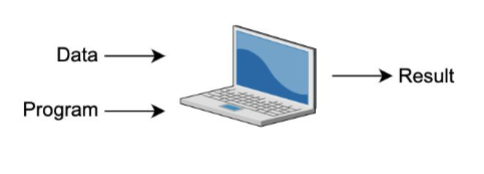
\includegraphics[width=0.5\linewidth]{symbolic.png}
    \caption{Symbolic Approach}
    \label{fig:enter-label}
\end{figure}
\begin{enumerate}
    \item \textbf{Key Characteristics}:
    \begin{enumerate}
        \item \textbf{"Model the knowledge of an adult"}
        \item \textbf{Symbol Manipulation}: The approach focuses on manipulating symbols according to predefined rules and logic.
        \item \textbf{Knowledge Representation}: Information is represented using explicit symbols, which can represent concepts, relationships, and facts.
        \item \textbf{Rule-Based Systems}: AI systems in this approach often use rule-based systems to infer conclusions from given premises.
        \item \textbf{Logic and Inference}: Logical reasoning is a core component of this approach, and it's used to derive new information from existing knowledge.
        \item \textbf{Expert Systems}: Early AI applications like expert systems used the symbolic approach, where human expertise was encoded in the form of rules and facts.
    \end{enumerate}
    \item \textbf{Strengths}:
        \begin{enumerate}
        \item \textbf{Transparency}: Symbolic systems provide a clear and interpretable representation of knowledge and reasoning processes.
        \item \textbf{Logical Reasoning}: Well-suited for problems that require logical inference and deductive reasoning.
        \item \textbf{Human-Readable}: The representations used are often human-readable and understandable.
    \end{enumerate}
    \item \textbf{Weaknesses}:
            \begin{enumerate}
        \item \textbf{Complexity}: Symbolic approaches can struggle with managing and representing the complexity of real-world domains.
        \item \textbf{Knowledge Acquisition}: Constructing a comprehensive set of rules and knowledge for complex domains can be challenging.
        \item \textbf{Lack of Contextual Understanding}: Symbolic systems may struggle with tasks that require understanding context and handling ambiguous or incomplete information.
    \end{enumerate}
\end{enumerate}
    \item \textbf{Connectionist Approach}
\begin{definition}
The \textbf{connectionist} approach, also known as the \textbf{neural network} approach, draws inspiration from the \textbf{structure and function of the human brain}. It involves building \textbf{artificial neural networks} that consist of \textbf{interconnected nodes (neurons)} that process information in a parallel and distributed manner. These networks learn patterns and relationships from data through \textbf{training processes} that adjust the strengths of connections (weights) between neurons.
\end{definition}
\begin{figure}[h!t]
    \centering
    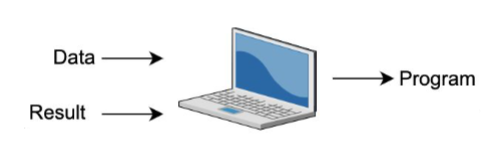
\includegraphics[width=0.5\linewidth]{connectionist.png}
    \caption{Connectionist Approach}
    
    \label{fig:enter-label}
\end{figure}
\begin{enumerate}
    \item \textbf{Key Characteristics}:
    \begin{enumerate}
        \item \textbf{"Simulate the learning of a baby"}
        \item \textbf{Parallel Distributed Processing}: Information processing occurs in parallel across interconnected nodes, leading to emergent properties.
        \item \textbf{Learning from Data}: Neural networks learn patterns and relationships from large datasets through processes like supervised learning, unsupervised learning, and reinforcement learning.
        \item \textbf{Feature Extraction}: Neural networks can automatically learn relevant features from raw data, reducing the need for hand-crafted feature engineering.
        \item \textbf{Nonlinear Mapping}: Neural networks can capture complex nonlinear relationships in data.
    \end{enumerate}
    \item \textbf{Strengths}:
        \begin{enumerate}
        \item \textbf{Pattern Recognition}: Excellent at tasks such as image recognition, natural language processing, and other tasks involving pattern recognition.
        \item \textbf{Adaptability}: Neural networks can learn from data and adapt to different tasks with appropriate training.
        \item \textbf{Robustness}: Neural networks can generalize well to new data, even in the presence of noise or variability.
    \end{enumerate}
    \item \textbf{Weaknesses}:
            \begin{enumerate}
        \item \textbf{Black Box Nature}: Neural networks can be challenging to interpret, and understanding their decision-making processes can be difficult.
        \item \textbf{Data Dependency}: Neural networks require substantial amounts of data for effective training.
        \item \textbf{Overfitting}: There's a risk of overfitting to training data if not properly regularized.
    \end{enumerate}
\end{enumerate}
\end{enumerate}
AI researchers tend to avoid the term as much as possible, and talk about much more specific, relatively well-defined fields:
\begin{itemize}
    \item \textbf{Machine Learning (ML)}: developing algorithms that learn from data rather than being hard-coded to solve a task
    \item \textbf{Computer Vision (CV)}: making computers capable of seeing
    \item \textbf{ (NLP)}: making computers capable of understanding our languages

\end{itemize}
Until recently, these fields were almost completely separate. All of these are now dominated by Deep Learning.\\
\\\textbf{Machine Learning} enables computers to \textbf{learn} from data, \textbf{rather than being explicitly programmed}, to solve a task. ML is a very broad term. There are many methods of learning from data. We need machine learning because almost every rule will have some counter-example in the real world. This makes it difficult to cover all conditions in an algorithm. High-dimensional input space, like colored images are hard to understand, and require us to first learn easier representations. We require a way to learn from a lot of examples to solve a problem.\\

\textbf{General Machine Learning Approach:}
\begin{enumerate}
    \item \textbf{Identify information} we want to find
    \item \textbf{Collect data} that will hold that information
    \item Design and run \textbf{algorithms to extract} as much information possible from data
\end{enumerate}

\begin{idea}
"A computer program is said to learn from experience \textbf{E} with respect to
some class of tasks \textbf{T} and performance measure \textbf{P}, if its performance at tasks
in \textbf{T}, as measured by \textbf{P}, improves with experience\textbf{ E}." (Mitchell et al. 1997)
\end{idea}
\section{Deep Learning}
\textbf{Deep Learning} is the latest version of \textbf{Artificial Neural Networks (ANN)}, or \textbf{Connectionism (an old ML method)}. Neural networks were inspired by the \textbf{brain}.
\begin{figure}[h!t]
    \centering
    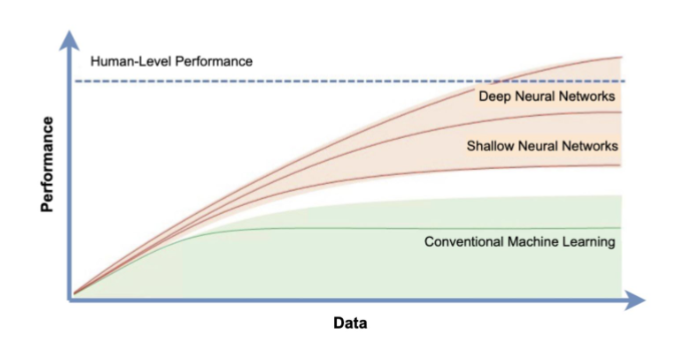
\includegraphics[width=0.75\linewidth]{deeplearning.png}
    \caption{Deep Learning}
    
    \label{fig:enter-label}
\end{figure}
\begin{definition}
"\textbf{Deep learning} is a subset of machine learning that allows \textbf{multiple levels of
representation}, obtained by composing simple but \textbf{non-linear modules} that
each transform the representation at one level \textbf{(starting with the raw input)}
into a representation at a higher, slightly more \textbf{abstract level}." (LeCun et al. 2015)
\end{definition}
\begin{figure}[h!t]
    \centering
    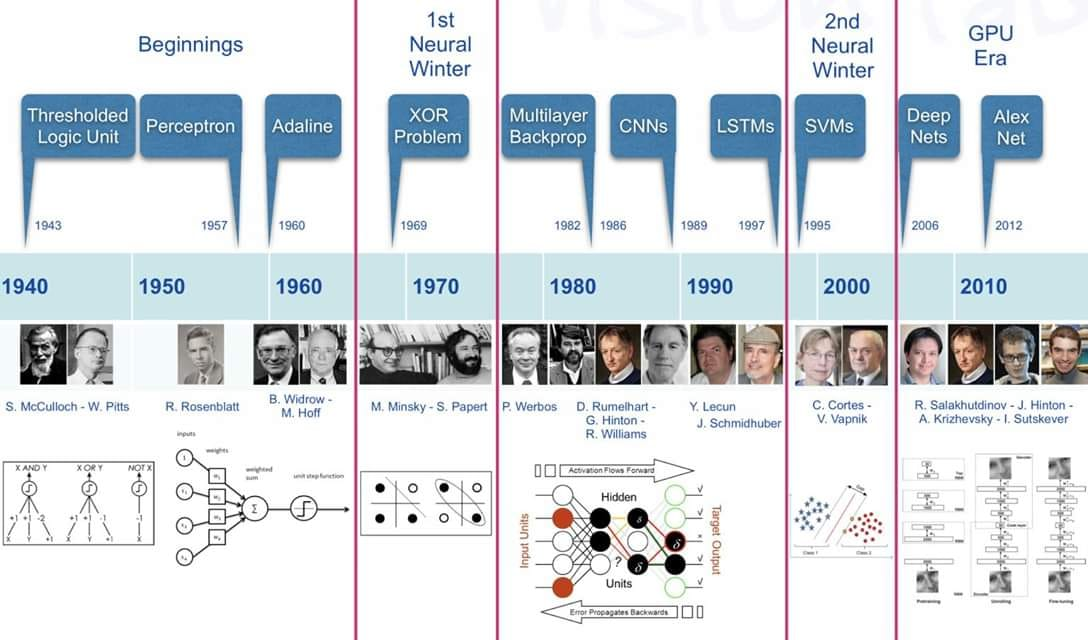
\includegraphics[width=0.75\linewidth]{historydeeplearning.png}
    \caption{History of Deep Learning}
    \label{fig:enter-label}
\end{figure}
\begin{definition}
    \textbf{Artificial Intelligence (AI)}: broad and poorly defined concept of developing computer systems that can \textbf{perform tasks normally only humans could do}. 
\end{definition}
\begin{definition}
    \textbf{Machine Learning (ML)}: computers \textbf{learn by example, from data}, rather than being explicitly programmed, to solve a task. 
\end{definition}
\begin{definition}
    \textbf{Deep Learning (DL)}: a machine learning method that learns \textbf{multiple levels of abstractions} over data end-to-end.
\end{definition}
\begin{figure}[h!t]
    \centering
    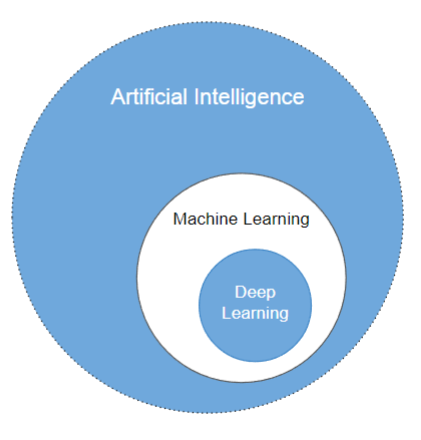
\includegraphics[width=0.25\linewidth]{aimldl.png}
    \caption{Artificial Intelligence vs. Machine Learning vs. Deep Learning}
    \label{fig:enter-label}
\end{figure}
\textbf{\\Deep Learning: Successes}
\begin{itemize}
    \item Machine Translation (Google Translate)
    \item Drug Discovery (antibiotics)
    \item Speech Recognition (auto-generated subtitles)
    \item Image Generation (generate image from prompts)
    \item AlphaFold (protein structures)
    \item AlphaGo
    \item Mathematics (pattern discovery)
    \item Code Generation
    \item Language Modelling
    \item Simulators
\end{itemize}
\textbf{Deep Learning: Caveats}
\begin{itemize}
    \item Interpretability (black box)
    \item Adversarial Examples (noise filters over images)
    \item Causality (while deep learning models excel at identifying patterns in data, they fall short in distinguishing between correlation and causation)
    \item Fairness and Bias
\end{itemize}
\begin{definition}
    \textbf{Bias:} refers to \textbf{systematic and consistent errors or inaccuracies in the predictions or outcomes} produced by a machine learning model. These biases can arise from \textbf{various sources} and can significantly \textbf{impact the model's performance and fairness}. Bias in deep learning can \textbf{occur at different stages} of the model development process, including \textbf{data collection}, \textbf{preprocessing}, \textbf{algorithm design}, and \textbf{decision-making}. 
\end{definition}
\begin{example}
    A 2016 arXiv paper, claimed to be able to predict whether someone was a convicted criminal or not solely from a driver's license-style photo with 90\% accuracy.
When looked at in detail, images of criminals were collected from government IDs, while non-criminal face images were collected from the internet.
\end{example}
    \begin{figure} [h!t]
        \centering
        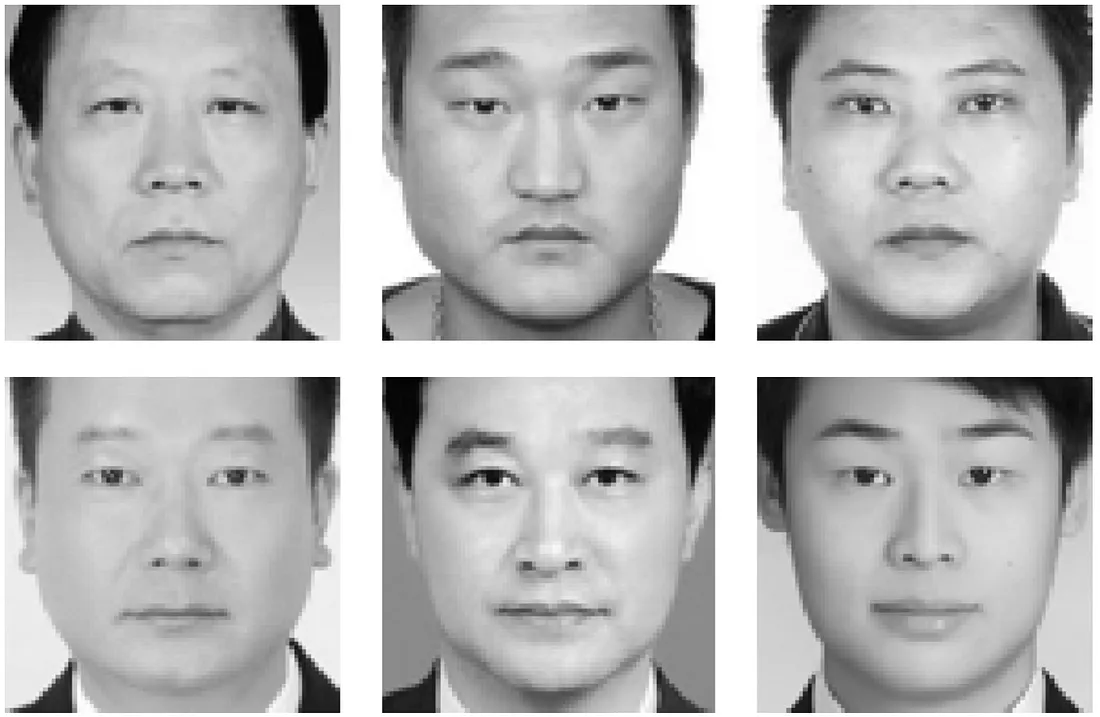
\includegraphics[width=0.5\linewidth]{criminalexamples.png}
        \caption{Top: "criminal" images. Bottom: "non-criminal" images.}
        
    \end{figure}
\section{Machine Learning Basics}

There are three categories that describe how a Neural Network "learns":

\begin{enumerate}
    \item \textbf{Supervised Learning}
\begin{definition}
    \textbf{Supervised Learning:} training by feeding \textbf{labeled data} to the computer, leading it to \textbf{predict the correct label} for inputted data (relationship between input and label)
\end{definition}
\begin{itemize}
\item Involves two main tasks: 
\begin{enumerate}
    \item \textbf{Regression}: the model predicts a continuous or real-valued output
    \item \textbf{Classification}: the model assigns inputs to specific categories or classes
\end{enumerate}
\item Performance is often measured using metrics like \textbf{mean squared error} (for regression) or \textbf{accuracy, precision, and recall (true positive rate) }(for classification)
\item Requires data with \textbf{ground-truth labels}
\end{itemize}
\begin{definition}

            \textbf{Mean Squared Error (MSE):} metric used for measuring the \textbf{average squared difference} between the \textbf{predicted values} and the \textbf{actual (true) values} in a regression problem. It provides a measure of how well a regression model's predictions align with the \textbf{ground truth values}. The lower the MSE value, the better the model's predictions match the data points.\\

\[ \text{MSE} = \frac{1}{n} \sum_{i=1}^{n} (y_i - \hat{y}_i)^2 \]

Where:
\begin{itemize}
\item  \( n \) is the number of data points (samples) in the dataset.
\item \( y_i \) represents the actual target value (ground truth) for the \( i \)th data point.
\item \( \hat{y}_i \) represents the predicted value for the \( i \)th data point by the regression model.
\end{itemize}
\end{definition}

\begin{definition}
    \textbf{Accuracy:} metric that measures the \textbf{proportion of correct predictions} made by a classification model/ It gives an overall view of the model's correctness across all classes.\\
\[ \text{Accuracy} = \frac{\text{Number of Correct Predictions}}{\text{Total Number of Predictions}} \]
\end{definition}

\begin{warning}
Accuracy can be misleading in cases where \textbf{classes are imbalanced}. If one class is significantly more prevalent than others, a model might achieve high accuracy by simply predicting the majority class for all instances.
\end{warning}

\begin{definition}
    \textbf{Precision:} metric that measures the \textbf{proportion of positive predictions} that were actually correct. It measures the model's \textbf{ability to avoid false positives} (instances tat were predicted as positive but are actually negative).\\
\[\text{Precision} = \frac{\text{True Positives}}{\text{True Positives + False Positives}} \] 
\end{definition}

\begin{definition}
    \textbf{Recall (True Positive Rate):} metric that quantifies the \textbf{proportion of actual positive instances} that were correctly predicted by the model. It helps identify the model's ability to \textbf{capture all instances of the positive class}, minimizing false negatives (instances that are actually positive but are predicted as negative). \\
\[ \text{Recall} = \frac{\text{True Positives}}{\text{True Positives + False Negatives}}\]
\end{definition}



\begin{example}
    \textbf{Fitting a polynomial (Regression):} Given a noise sample data (blue), we want to find the polynomial that generated the data.
However, many possible curves fit. Which of these curves is the best fit and why? This is where knowledge of the problem, \textbf{domain knowledge}, can be used to select an appropriate modelling technique.
\end{example}
\begin{figure}[h!t]
    \centering
    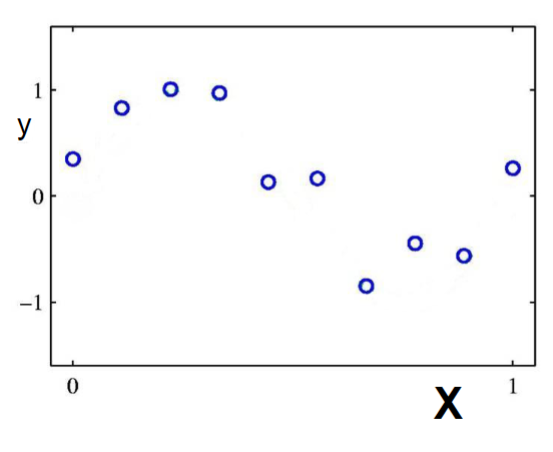
\includegraphics[width=0.5\linewidth]{regressionexample1.png}
    \caption{Noisy Sample Data}
    \label{fig:enter-label}
\end{figure}
\begin{figure}[h!t]
    \centering
    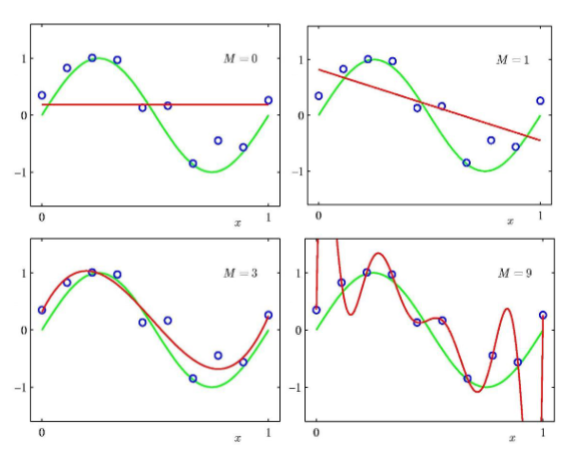
\includegraphics[width=0.5\linewidth]{possiblecurves.png}
    \caption{Possible Curves}
    \label{fig:enter-label}
\end{figure}

\begin{definition}
    \textbf{Inductive Bias (Learning Bias):} set of \textbf{assumptions} used for modelling, or prior knowledge that a learning model \textbf{uses to generalize} from the training data to new, unseen data. It's the foundational principles and constraints that guide a model's learning process and influence the types of patterns it's more likely to learn. Applies to all types of learning.
\end{definition}

\begin{theorem}
\textbf{No Free Lunch Theorem:} concept that \textbf{there is no universal optimization} of learning algorithm that performs best for all possible problems. There is \textbf{no one-size-fits-all approach} that can excel across all domains and problem instances.
\end{theorem}

    \item \textbf{Unsupervised Learning}
\begin{definition}
  \textbf{ Unsupervised Learning:}  training by feeding \textbf{unlabeled data}; hence, relationships are made between \textbf{elements of input} (Clustering, grouping algorithm)
\end{definition}
\begin{itemize}
    \item Requires observations\textbf{ without human annotations}
    \item Also known as Self-supervised Learning or Semi-supervised Learning
\end{itemize}
    \item \textbf{Reinforcement Learning}
\begin{definition}
    \textbf{Reinforcement Learning:} when we want to train a computer to perform a task but \textbf{we don’t know the optimized way} so the computer \textbf{finds the best steps by itself} (we rank the computer’s methods relative to each other and this way the computer learns the best method to perform a task)
\end{definition}
\begin{itemize}
    \item Has an\textbf{ agent}, which is an entity capable of perceiving its environment, making decisions, and taking actions in order to achieve specific goals. This may be a software program, a robot equipped with sensors, or any \textbf{system that interacts with its environment} to acheive desired outcomes. 
    \item \textbf{Sparse rewards} from environment. For example, winning or losing can only occur at the end of a game, making it difficult for an agent to learn to specific actions that lead to victory.
    \item \textbf{Dynamic nature}: agent's actions directly influence the environment. \textbf{Feedback loop} where agent's actions influence the environment, which in turn affects the agent's future options and decisions.

\end{itemize}

\end{enumerate}

\textbf{Machine Learning is a game of balance, with the objective being to generalize training data and future data.}

\begin{definition}
\textbf{Bias:} refers to the \textbf{error introduced by approximating a real-world problem}, which may be complex, with a simplified model. In the context of a machine learning model, bias is the \textbf{error due to overly simplistic assumptions in the learning algorithm}. If a model has high bias, it means that it doesn't capture the underlying patterns in the training data well, leading to systematic errors. In other words, it is "\textbf{underfitting}" the data.
\end{definition}
    
\begin{definition}
\textbf{Variance:} refers to the model's \textbf{sensitivity to small fluctuations or changes} in the training data. A model with high variance tends to fit the training data very closely, even capturing noise or randomness in the data. This can lead to a situation where the model performs well on the training data but poorly on new, unseen data, because it \textbf{hasn't generalized well}. This is called "\textbf{overfitting}."
\end{definition}

\begin{theorem}
    \textbf{Bias-Variance Tradeoff}: as you increase the complexity of a model, you generally reduce bias but increase variance, and vice versa. Finding the right level of complexity that minimizes both bias and variance is crucial for building models that generalize well to new data.

    \begin{itemize}
        \item If you \textbf{increase model complexity} (more features, more layers in neural networks, etc.), the model becomes more flexible and capable of fitting the training data closely. However, it also becomes more sensitive to fluctuations and noise in the data, \textbf{increasing the risk of overfitting} (high variance).
        \item If you\textbf{ decrease model complexity}, the model becomes more constrained and less likely to fit the training data perfectly. While it might generalize better to new data, it could struggle to capture complex patterns, \textbf{resulting in underfitting} (high bias).
    \end{itemize}
\end{theorem}
\begin{idea}
    Generally, \textbf{more data} leads to a better model.
\end{idea}

We need to split our dataset so that it can be use to\textbf{ train, validate, and test }the model. We need to ensure the model does not see the testing (holdout) data during the training process, as that leads to overfitting to the test data and poor generalization on new data. The purpose of validation data is for assessing performance and making informed decisions about model selection and hyper-parameter tuning. 

\begin{figure}[h!t]
    \centering
    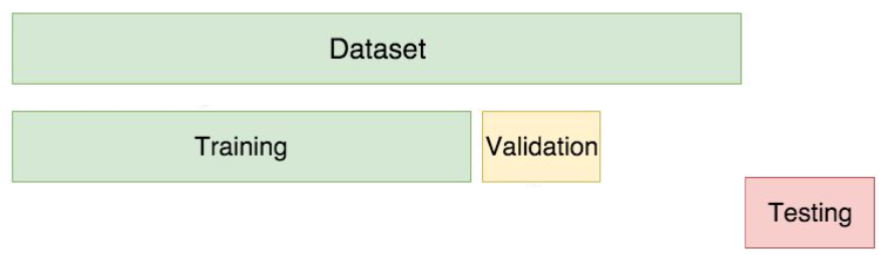
\includegraphics[width=0.75\linewidth]{datatypes.png}
    \caption{Dataset split into Training, Validation, and Testing Datasets}
    \label{fig:enter-label}
\end{figure}


\chapter{Artificial Neural Networks (ANNs)}
\begin{idea}
\begin{itemize}
\item \textbf{Artificial Neural Networks (ANNs):} Computational models inspired by the brain's structure and function.
\item \textbf{Neurons:} Processing units in ANNs that apply weights to inputs and pass through activation functions.
\item \textbf{Activation Functions:} Introduce non-linearity to neuron outputs, enabling complex pattern capturing.
\item \textbf{Loss Function:} Measures the discrepancy between predicted and actual outputs.
\item \textbf{Training:} Process of adjusting weights to minimize the loss function.
\item \textbf{Gradient Descent:} Optimization algorithm that updates weights in the direction of loss reduction.
\item \textbf{Simple Fully Connected Network:} Neurons in one layer connected to all in the next; input passes through hidden layers to produce output.
\item \textbf{Hyperparameters:} Settings chosen prior to training, such as learning rate, batch size, and network architecture.
\item \textbf{Optimizers:} Algorithms that control weight updates during training (e.g., SGD, Adam).
\item \textbf{Normalization:} Techniques like Batch Norm and Layer Norm stabilize training by normalizing input or activation distributions.
\item \textbf{Regularization:} Techniques like Dropout and Weight Decay prevent overfitting by adding constraints or penalties.
\end{itemize}
\end{idea}

\section{Neuron}

\textbf{Simplified Biological Neuron:}
\begin{itemize}
    \item \textbf{Dendrites} recieve information from other neurons
    \item \textbf{Cell body} consolidates information from the dendrites
    \item \textbf{Axon} passes information to other neurons
    \item \textbf{Synapse} is the area where the axon of one neuron and the dendrite of another connect
\end{itemize}

\begin{figure} [h!t]
    \centering
    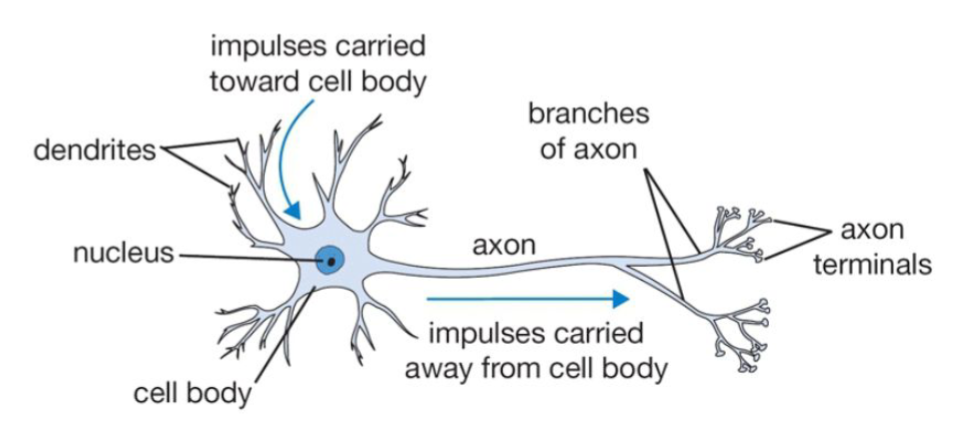
\includegraphics[width=0.5\linewidth]{bioneuron.png}
    \caption{Simplified Biological Neuron}
    \label{fig:enter-label}
\end{figure}

Neurons \textbf{fire} on stimuli: edges, lines, angles, movements, familiar faces, etc. regardless of scale, rotation and translation.\\

\textbf{Artificial Neuron}:

\begin{itemize}
    \item $\mathbf{x}_i$ is the \textbf{input} such as a pixel in an image
    \item $\mathbf{w}_i$ is the \textbf{weight} for input $\mathbf{x}_i$ that we learn for this particular input
    \item $\mathbf{b}$ is the \textbf{bias}, a weight we learn with no input
    \item $\mathbf{f}$ is the \textbf{activation function} that determines how our output changes with the sum of all weight-input products
    \item $\mathbf{y}$ is the\textbf{ output} such as the class an image belongs to
\begin{figure}[h!t]
    \centering
    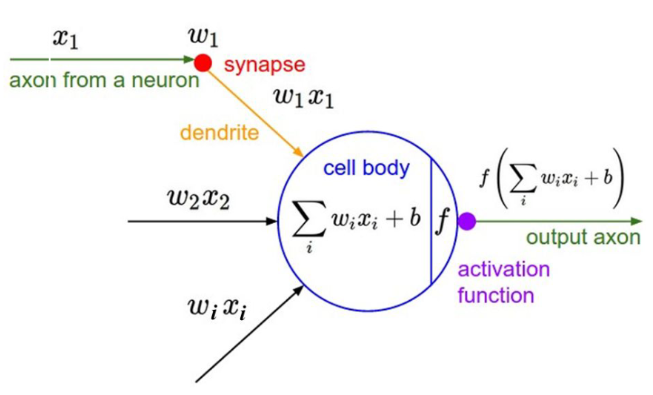
\includegraphics[width=0.5\linewidth]{artificialneuron1.png}
    \caption{Mathematical Representation of Artificial Neuron}
    \label{fig:enter-label}
\end{figure}
    \item Basically, we take the \textbf{weighted sum of all inputs}, \textbf{add the bias term}, then pass the result to the \textbf{activation function}. The result of the activation function is the \textbf{output}.
\[ \Huge y = f(w \cdot x + b) \]

\end{itemize}
\begin{figure} [h!t]
    \centering
    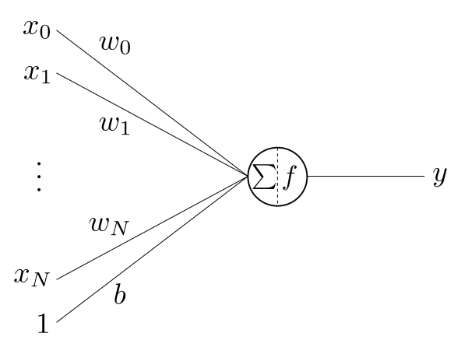
\includegraphics[width=0.5\linewidth]{artificialneuron2.png}
    \caption{Vector Representation of Artificial Neuron}
    \label{fig:enter-label}
\end{figure}
\section{Activation Function}

\textbf{Linear Activation Function}
\begin{definition}
    \textbf{Linear Activation Function}: a mathematical function that produces an \textbf{output directly proportional to its input}. In other words, for any given input, the output increases or decreases at a constant rate without any bending or non-linear behavior.
\end{definition}
\begin{figure}[h!t]
    \centering
    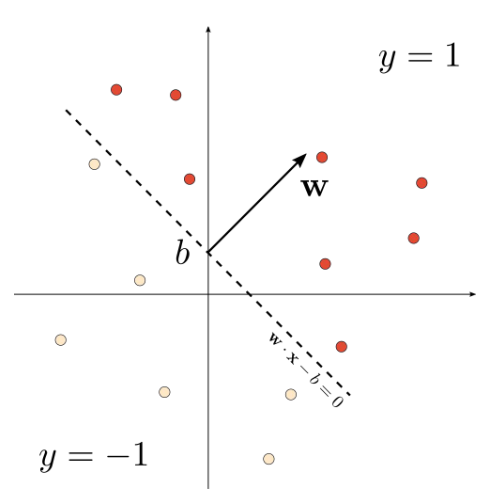
\includegraphics[width=0.4\linewidth]{linearactivation.png}
    \caption{Linear Activation Function}
    \label{fig:enter-label}
\end{figure}
\begin{itemize}
    \item When the activation function is a simple linear function:
\[ y = f(w \cdot x + b) \longrightarrow y = w \cdot x + b\]
    \item This is a special equation and becomes more clear if we write it out for 2D:
\[y = w_0 x_0 + w_1 x_1 + b\]
    \item Recall general equation of line:

\[Ax + By - C = 0\]

    \item The bias is related to the offset of the line from the origin and allows us to create a boundary between data that doesn't have to go through the origin
\begin{definition}
   \textbf{ Bias Term:} a \textbf{constant} value that's added to the weighted sum of inputs in a neuron or model, allowing the neuron to \textbf{shift the activation function's output} up or down, effectively \textbf{adjusting the decision boundary} of the neuron's response. The bias term is \textbf{learnable} during the training process, just like the weights associated with the inputs
\end{definition}
    \item \(y = w \cdot x + b\)  is a generalized line for any dimension, known as \textbf{hyperplane}, splitting the n-dimensional input space into 2 parts
    \item Linear activation functions are \textbf{not usually practical} since most real datasets are not linearly separable (we can't usually find a straight line that separates classes well in a classification problem)
    \item We can learn \textbf{non-linear transformations} of our data to help
\begin{figure}[h!t]
        \centering
        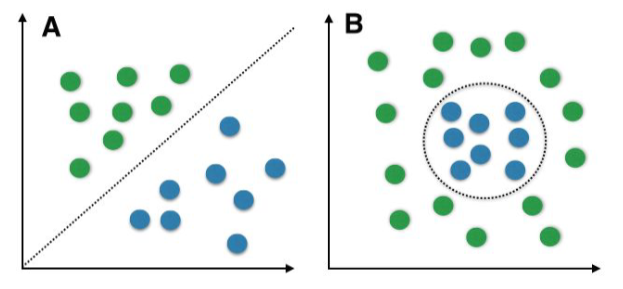
\includegraphics[width=0.5\linewidth]{linearvsnonlinearAF.png}
        \caption{Most datasets are not linearly separable like A}
        \label{fig:enter-label}
    \end{figure}
    \item Multiple layers with non-linear transformations are useful, while \textbf{there is no advantage from multiple linear layers}, since the composite is a linear layer and reduces the network's ability to capture complex patterns in data
\end{itemize}
\textbf{Perceptrons (Binary Activation Function)}
\begin{definition}
   \textbf{ Perceptron Activation Function:} a decision rule that outputs \textbf{1 when the weighted sum of inputs exceeds a threshold, and outputs 0 otherwise}. This decision guides the activation of a perceptron in a basic neural network unit.
\end{definition}
\begin{figure}[h!t]
    \centering
    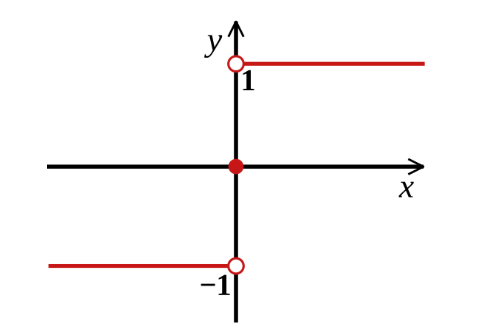
\includegraphics[width=0.4\linewidth]{perceptrons.png}
    \caption{Perceptrons}
    \label{fig:enter-label}
\end{figure}
\begin{itemize}
\item The first artificial neurons (1943-1970s) use a simple binary activation function based on which side of the hyperplane the input is
\item Examples of these functions include the \textbf{Sign function} and the \textbf{Heaviside (unit) step function}
\[f(x) = sign(x)\]
\[f(x) = \begin{cases}
        0, & \text{if } x < 0, \\
        1, & \text{if } x \geq 0.
      \end{cases}\]
      \item The \textbf{decision boundary} is the hyperplane, or the \textbf{threshold that separates the classes} in the binary classification problem. 
      \item These functions are \textbf{not differentiable, contiuous or smooth}


\end{itemize}
\textbf{Sigmoid Activation Function}
\begin{figure}[h!t]
    \centering
    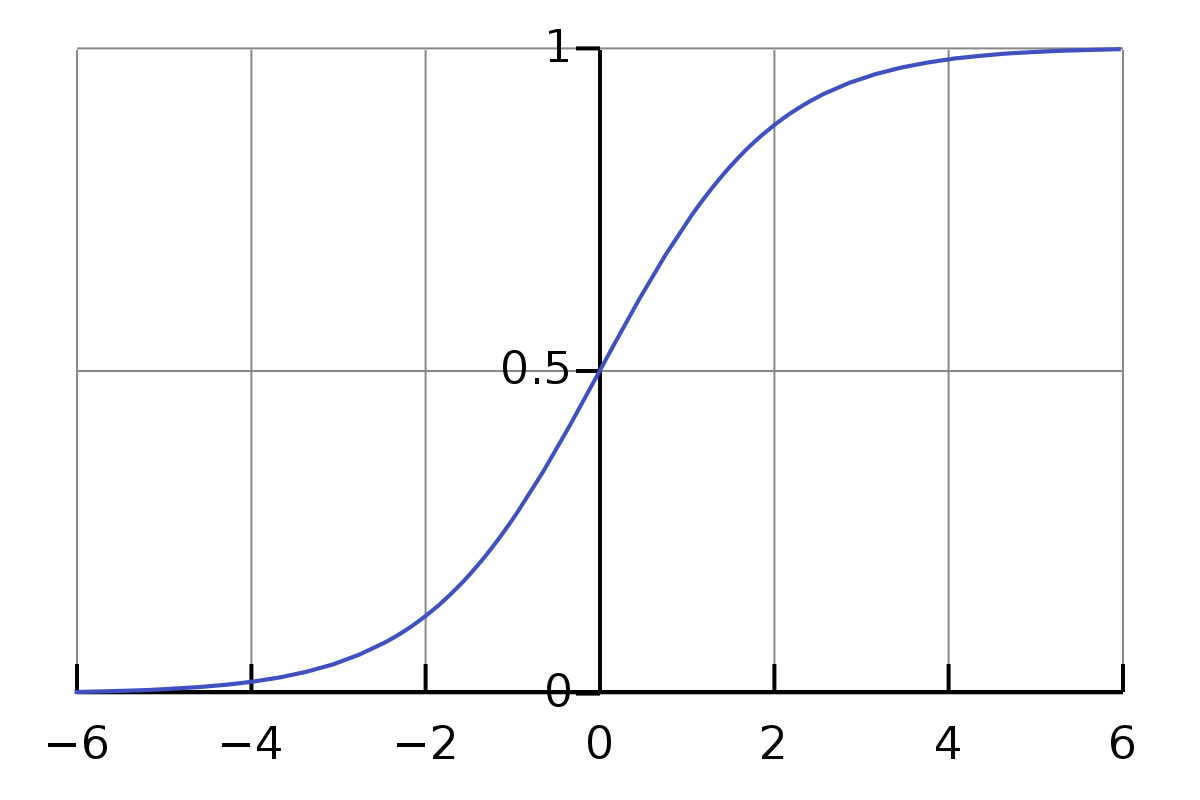
\includegraphics[width=0.5\linewidth]{sigmoid.png}
    \caption{Sigmoid Function}
    \label{fig:enter-label}
\end{figure}
\begin{definition}
    \textbf{Sigmoid Activation Function:} a mathematical function that \textbf{smoothly} maps input values to a specified output range. It is characterized by an S-shaped curve and is commonly used in neural networks to \textbf{introduce non-linearity}, allowing the network to capture complex relationships in data. The sigmoid function is particularly useful for transforming raw scores into probabilities or for controlling the strength of neuron activations.
\end{definition}
\begin{itemize}
    \item Sigmoid activation functions were most common before 2012
    \item \textbf{Easily differentiable, smooth, continuous}
    \item Range between [-1, 1] or [0, 1]
    \item There are many sigmoid functions, the most common are \textbf{Hyperbolic tangent} and \textbf{Logistic functions}:

\[f(x) = \text{tanh}(x)\]

\[f(x) = \frac{1}{1 + e^{-x}}\]
\item Saturated neurons "kill" the gradients
\begin{definition}
    \textbf{Gradients:} represent the directions and magnitudes by which the network's internal settings (weights and biases) should be adjusted to minimize the difference between its predictions and the actual target values. Gradients guide the network during training, helping it learn how to make better predictions by fine-tuning its parameters based on the errors it makes.
\end{definition}
\item Gradients become vanishingly small very quickly away from x = 0
\begin{theorem}
    \textbf{Vanishing Gradient Problem:}  pertains to the phenomenon wherein the \textbf{gradients of the loss function} with respect to the parameters of the earlier layers \textbf{become extremely small} as they are back-propagated through the network during the learning process. This reduction in gradient magnitude \textbf{diminishes the weight updates applied to the earlier layers} during optimization, causing these layers to \textbf{learn at a significantly slower rate or even stagnate} in terms of learning progress. As a consequence, the \textbf{network struggles to capture complex relationships} in the data, hindering its ability to generalize and make accurate predictions.
\end{theorem}
\end{itemize}
\begin{figure}[h!t]
    \centering
    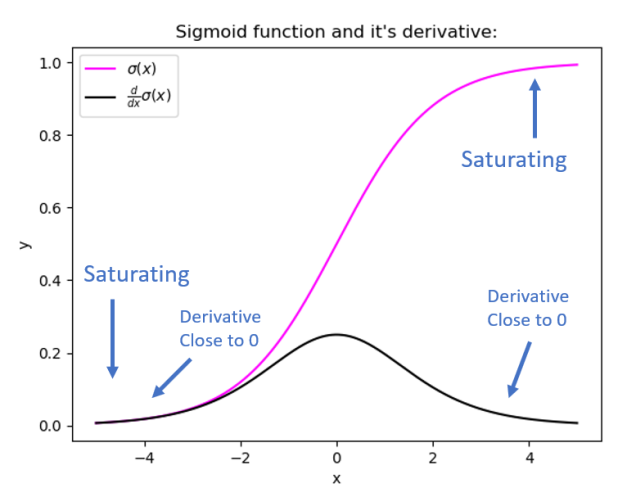
\includegraphics[width=0.5\linewidth]{vanishinggradientproblem.png}
    \caption{Vanishing Gradient Problem}
    \label{fig:enter-label}
\end{figure}

\newpage

\textbf{ReLU Activation Function}

\begin{definition}
\textbf{ ReLU Activation Function:} turns \textbf{on for positive input values}, allowing signals to pass unchanged. For \textbf{negative inputs, it outputs zero}, which helps the network introduce non-linearity and learn complex patterns in data. ReLU helps with the vanishing gradient problem, though variations like Leaky ReLU address potential issues of inactive neurons during training.
\end{definition}

\begin{figure}[h!t]
    \centering
    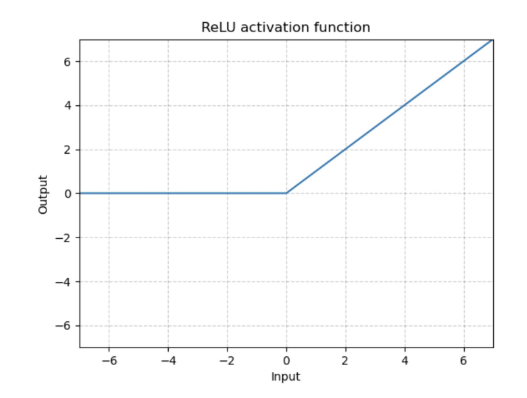
\includegraphics[width=0.5\linewidth]{ReLU.png}
    \caption{ReLU Activation Function}
    \label{fig:enter-label}
\end{figure}

\begin{itemize}
    \item Modern deep learning typically uses the \textbf{Rectified Linear Unit (ReLU)} based activation functions:
    \begin{itemize}
        \item \textbf{ReLU}:

\[\text{ReLU}(x) = (x)^+ = \max(0, x)\]

        \item \textbf{Leaky ReLU}:

\[
\text{LeakyReLU}(x) = \begin{cases}
x, & \text{if } x \geq 0 \\
\text{negative\_slope} \cdot x, & \text{otherwise}
\end{cases}\]


        \item \textbf{Parametric ReLU:}

\[\text{PReLU}(x) = \begin{cases}
x, & \text{if } x \geq 0 \\
a \cdot x, & \text{otherwise}
\end{cases}\]
\item These functions have very \textbf{easy derivaties}: 0 or 1; use 0 at x = 0
\end{itemize}
\item We can also approximate ReLU activation by \textbf{continuous functions}:
\begin{itemize}
    \item \textbf{SiLU (Swish)}:

\[\text{SiLU}(x) = x \cdot \sigma(x) = \frac{x}{1 + e^{-x}}\]

    \item \textbf{SoftPlus}:


\[\text{SoftPlus}(x) = \frac{1}{\beta} \cdot \log(1 + e^{\beta x})\]

    \item These work \textbf{on par or better} than ReLU functions  due to mitigating issues like the \textbf{vanishing gradient problem}, dead neurons, lack of smoothness, and noise sensitivity that can arise with the original ReLU function. These approximations offer improved stability, controlled activation behavior, and better optimization dynamics for specific tasks and network architectures.

\end{itemize}
\end{itemize}

\section{Training Neural Networks}

How do we learn the\textbf{ weights} and\textbf{ bias }of a neural network?\\
Input: \( x \), Predicted Output: \( y \), Ground Truth Label: \( t \), Neuron \( M(w;x) \)
\begin{enumerate}
  \item \textbf{Prediction:} Make a prediction for some input data \( x \), with a known correct output \( t \):
  \[ y = M(w;x) \]
  
  \item \textbf{Comparison:} Compare the correct output with our predicted output to compute loss:
  \[ E = \text{Loss}(y, t) \]
  
  \item \textbf{Adjustment:} Adjust the weights/bias to make the prediction closer to the ground truth, i.e., minimize error.
  \item \textbf{Repetiton:} Repeat until we have an acceptable level of error.

\end{enumerate}
This process gradually improves a network's ability to solve a problem.

\begin{definition}
    \textbf{Forward Pass:} input data is fed into a neural network, and it \textbf{flows through the layers}, undergoing computations using the network's parameters (weights and biases). This process generates predictions or output values based on the input data. Used for both \textbf{training and inference}.
\end{definition}

\begin{definition}
    \textbf{Backward Pass:} also known as \textbf{backpropagation}, this step follows the forward pass. It involves \textbf{calculating the gradients of the loss function} with respect to the network's parameters. These gradients indicate how much each parameter needs to be \textbf{adjusted} to reduce prediction errors. The gradients are then used to update the parameters using optimization algorithms. Used only for \textbf{training}.
\end{definition}

The forward pass is the initial step that \textbf{produces predictions} based on input data. The backward pass is crucial for \textbf{training} the network. By computing gradients during the backward pass, the network's parameters are adjusted in a way that \textbf{reduces prediction errors}. This adjustment is \textbf{iteratively repeated} through multiple forward and backward passes, refining the network's parameters to make better predictions over time.\\
\\In summary, the \textbf{forward pass generates predictions}, while the \textbf{backward pass calculates gradients to fine-tune the network's parameters}, enabling it to learn and improve its performance.

\begin{idea}
    All activation functions used in modern neural networks trained with backpropogation are both differentiable and non-linear.
\end{idea}

\section{Loss Function}
\begin{definition}
    \textbf{Loss Function:} computes \textbf{how bad predictions are} compared to the ground truth labels. Large loss means the network's predictions differ from the ground truth. Small loss means the network's prediction matches the ground truth.
\end{definition}

We want to calculate the error over \textbf{all training samples} (to get the average error).

\begin{figure}[h!t]
    \centering
    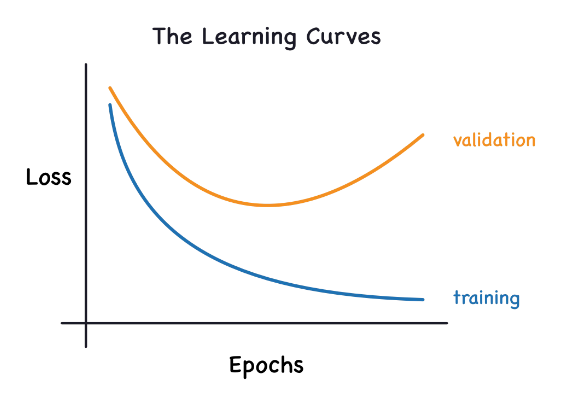
\includegraphics[width=0.25\linewidth]{lossfunction.png}
    \caption{Learning Curves}
    \label{fig:enter-label}
\end{figure}

\newpage

\begin{example}
    Suppose we want to train a linear neuron to differentiate images into three classes:
\end{example}
\begin{figure}[h!t]
    \centering
    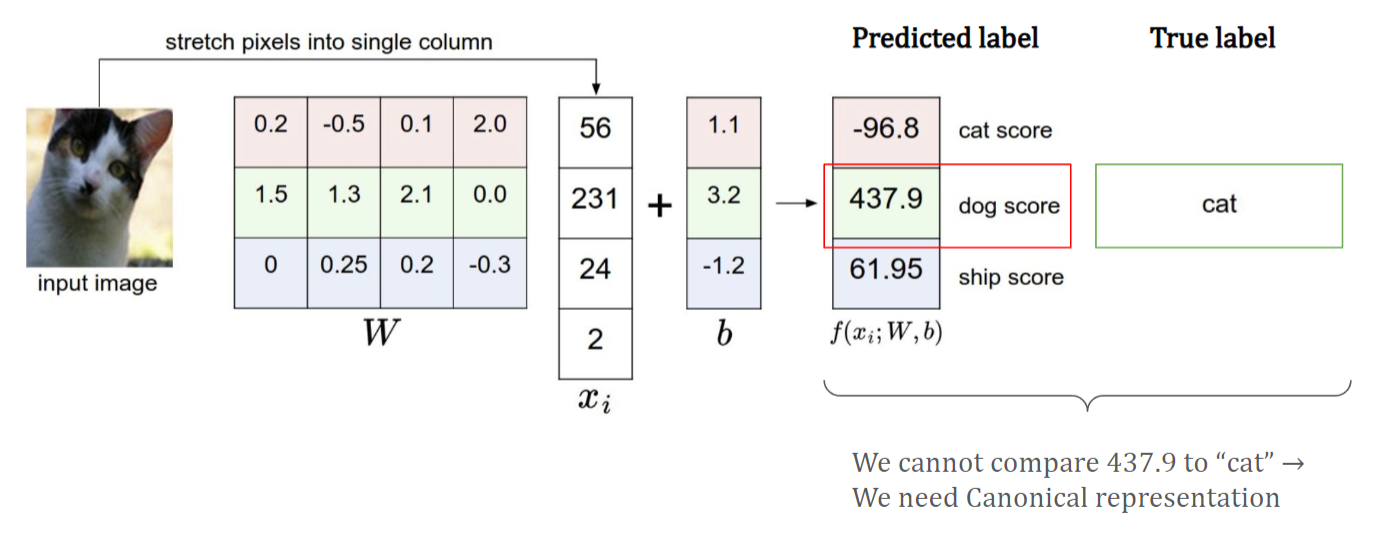
\includegraphics[width=0.75\linewidth]{whysoftmax.png}
    \caption{Why we need Softmax}
    \label{fig:enter-label}
\end{figure}
We need a way that will allow us to \textbf{represent the output} in a way that can be \textbf{compared to the true label} so that we may see if the model's predictions are accurate or not. Enter: \textbf{Softmax}.

\begin{definition}
    \textbf{Softmax function:} \textbf{normalizes the logits} into a categorical probability distribution over all possible classes. Produces normalized probabilites for multiple classes.
\end{definition}

\begin{figure}[h!t]
    \centering
    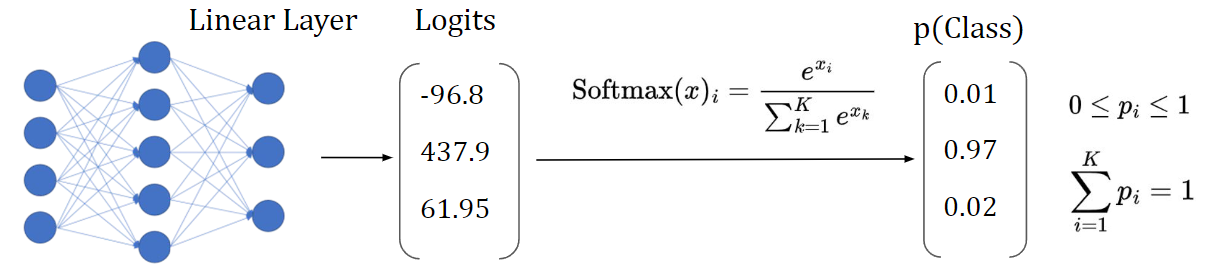
\includegraphics[width=0.75\linewidth]{softmax.png}
    \caption{Softmax Function}
    \label{fig:enter-label}
\end{figure}
We still need to map "cat" to a \textbf{vector} so that it can be compared with the softmax output. A way to map categories to vector representation is \textbf{One-hot encoding}.

\begin{definition}
    \textbf{One-hot encoding:}  a \textbf{binary representation} technique used to convert categorical variables into a \textbf{numerical format}. Each category is represented as a binary vector where a single element is set to \textbf{1} (indicating the \textbf{presence} of that category) while all other elements are set to \textbf{0} (indicating the \textbf{absence} of other categories).
\end{definition}
\begin{figure}[h!t]
    \centering
    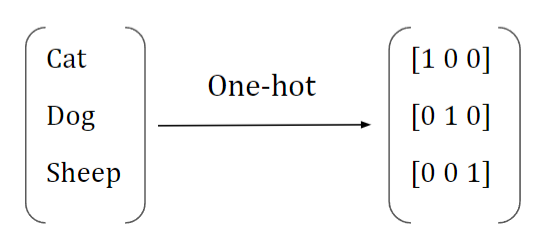
\includegraphics[width=0.25\linewidth]{onehotencoding.png}
    \caption{One-hot encoding}
    \label{fig:enter-label}
\end{figure}
Now that the output of the model and the classes have been converted to comparable forms, how do we determine the accuracy of the model? We use \textbf{Loss functions}:
\begin{enumerate}
    \item \textbf{Mean Squared Error (MSE)}: mostly used for \textbf{regression} problems (predicting continuous numeric output)
\[
MSE = \frac{1}{N} \sum_{n=1}^{N} (y_{\text{predicted}, i} - y_{\text{actual}, i})^2
\]

Where:
\begin{align*}
n &: \text{Number of data points (training samples)} \\
y_{\text{predicted}, i} &: \text{Predicted value for the } i\text{th data point} \\
y_{\text{actual}, i} &: \text{Actual target value for the } i\text{th data point}
\end{align*}
\begin{figure}[h!t]
    \centering
    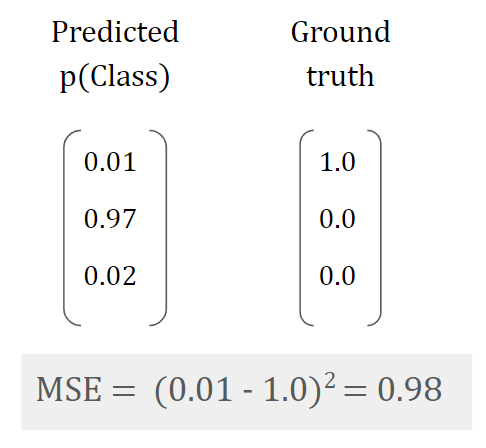
\includegraphics[width=0.25\linewidth]{mse.png}
    \caption{Mean Squared Error}
    \label{fig:enter-label}
\end{figure}
    \item \textbf{Cross Entropy (CE)}: mostly used for \textbf{multi-class classification} problems
\[
CE = - \frac{1}{N} \sum_{n=1}^{N} \sum_{k=1}^{K}  y_{\text{actual}, n, k} \cdot \log(y_{\text{predicted}, n, k}) 
\]

Where:
\begin{align*}
N &: \text{Number of data points (training samples)} \\
K &: \text{Number of classes} \\
y_{\text{actual}, n, k} &: \text{Actual target value (1 or 0) for the } n\text{th data point and } k\text{th class} \\
y_{\text{predicted}, n, k} &: \text{Predicted probability for the } k\text{th data point belonging to the } k\text{th class} \\
\end{align*}
\begin{figure}[h!t]
    \centering
    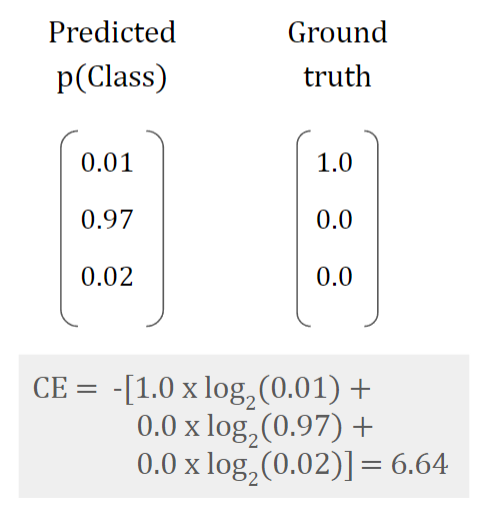
\includegraphics[width=0.25\linewidth]{ce.png}
    \caption{Cross Entropy Error}
    \label{fig:enter-label}
\end{figure}

    \item \textbf{Binary Cross Entropy (BCE)}: mostly used for \textbf{binary classification} problems
\[
BCE = -\frac{1}{N} \sum_{n=1}^{N} \left( y_{\text{actual}, n} \cdot \log(y_{\text{predicted}, n}) + (1 - y_{\text{actual}, n}) \cdot \log(1 - y_{\text{predicted}, n}) \right)
\]

Where:
\begin{align*}
N &: \text{Number of data points} \\
y_{\text{actual}, n} &: \text{Actual target value (0 or 1) for the } n\text{th data point} \\
y_{\text{predicted}, n} &: \text{Predicted probability for the } n\text{th data point} \\
\end{align*}
\end{enumerate}

\section{Gradient Descent}
\begin{definition}
    \textbf{Gradient Descent:} an optimization algorithm used in machine learning to \textbf{iteratively} adjust the parameters of a model in the \textbf{direction that decreases the model's error}, guided by the \textbf{gradient} of the error with respect to those parameters.
\end{definition}

A neural network layer with two neurons: 
\[y_1 = f(w_1 \cdot x + b_1)\]
\[y_2 = f(w_2 \cdot x + b_2)\]
can represent a neural network easier with a \textbf{matrix} where each neuron's weight vector is a \textbf{row of the weight matrix W} and the input is a \textbf{column vector x}:
\[y=f(Wx+b)\]
This is relevant for debugging the dimensions of tensors.

\begin{figure}[h!t]
    \centering
    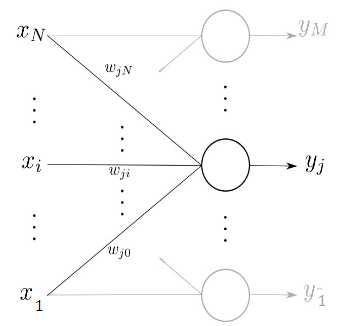
\includegraphics[width=0.3\linewidth]{twoneurons.png}
    \caption{NN layer represented by vectors}
    \label{fig:enter-label}
\end{figure}
In order to improve our network, we want to know how to change each of our neuron's weights \(w_ji\) to \textbf{reduce error} \(E\). Basically, we want to find the weights that are \textbf{increasing the error} and change them in the \textbf{opposite direction} of the current function to \textbf{correct} them. To do this, we will use \textbf{Gradient Descent}.

\begin{idea}
    In the context of this course, \textbf{gradients and derivatives are the same thing}. The \textbf{vector} of partial derivatives for all weights is the \textbf{gradient}. The \textbf{direction} of the gradient is the \textbf{direction the function is increasing}. The \textbf{magnitude} of the gradient is the \textbf{rate of increase}.
\end{idea}

First, we need to know how our error changes with \textbf{each individual weight}:
\[\frac{\partial E}{\partial w_{ji}}\]
This is relatively simple to calculate adjacent to the output layer. Adjusting weights according to the slope (gradient) will guide us to the minimum (or maximum) error. We do this by computing the \textbf{gradient of loss with respect to each weight}. That will tell us the direction in which the weight is increasing the loss.


\begin{figure}[h!t]
    \centering
    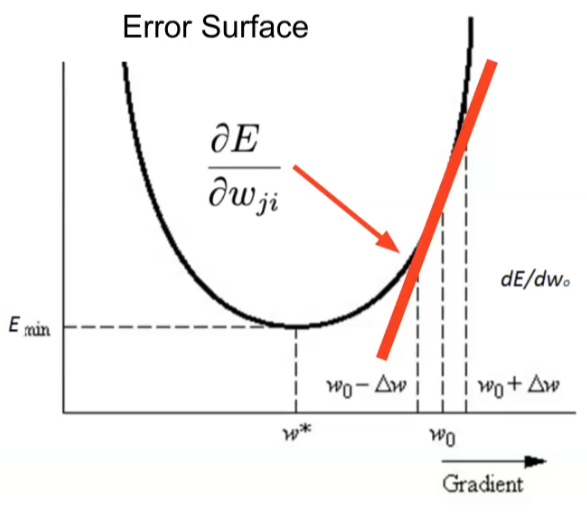
\includegraphics[width=0.5\linewidth]{gradientdescent.png}
    \caption{Gradient Descent. The graph represents the Error (loss) function and the red tangent line is gradient of loss.}
    \label{fig:enter-label}
\end{figure}


\[ \text{\textbf{Gradient Descent Formula:}    } w_{ji}^{t+1} = w_{ji}^{t} - \eta \frac{\partial E}{\partial w_{ji}}\]


\[\Delta w_{ji} = \eta \frac{\partial E}{\partial w_{ji}}\]


Where \(\eta\) is the learning rate (step size).\\

\begin{idea}
    A \textbf{positive} gradient at a weight means that the weight is\textbf{ contributing} to the loss. This is why we negate it in the Gradient Descent Formula
\end{idea}

\begin{example}
\textbf{Delta Rule} for Single Weight/Training Example


\[E = (y - t)^2  \text{  and  } f(x) = \frac{1}{1+e^{-x}}\]
To solve this, we need to use the \textbf{Chain Rule}:


\[ \frac{dE}{dw_p} = (\frac{dE}{dy}) (\frac{dy}{da}) (\frac{da}{dw_p}) \]
\begin{itemize}
    \item \(a = \sum_{p} w_p x_p + b\)    (summation of inputs)
    \item \(y = f(a)\)
    \item \(\frac{dE}{dw_p} \text{ represents the derivative of the error } E \text{ with respect to the weight } w_p.\)
    \item \(\frac{dE}{dy} \text{ represents the derivative of the error } E \text{ with respect to the output } y.\)
    \item \(\frac{dy}{da} \text{ represents the derivative of the output } y \text{ with respect to the input } a.\)
    \item \(\frac{da}{dw_p} \text{ represents the derivative of the input } a \text{ with respect to the weight } w_p.\)\\
\end{itemize}

Let's calculate each of these derivatives:


\[\frac{dE}{dy} = (\frac{d(y-t)^2}{dy}) = 2(y-t)\]


\[\frac{dy}{da} = (\frac{d{\frac{1}{1+e^{-a}}}}{da}) = (1-y)(y) \text{   (useful property of sigmoid functions)}\]

\[\frac{da}{dw_p} = x_p\]


\[\frac{dE}{dw_p} = 2(x_p)((y-t)((1-y)(y)))\]
\end{example}

\begin{figure}[h!t]
    \centering
    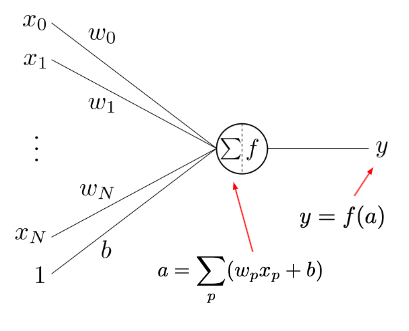
\includegraphics[width=0.4\linewidth]{deltaruleexample.png}
    \caption{Delta Rule Example}
    \label{fig:enter-label}
\end{figure}

\newpage

\section{Neural Network Architectures}

\textbf{XOR Problem}\\

\begin{figure} [h!t]
    \centering
    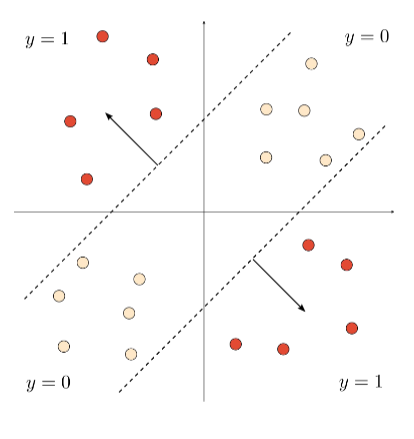
\includegraphics[width=0.35\linewidth]{xor.png}
    \caption{XOR Function}
    \label{fig:enter-label}
\end{figure}

Having a single decision boundary (a single NN layer) is not enough to solve many problems. The most famous such problem is the \textbf{XOR function}, which \textbf{needs two decision boundaries} to solve (more than one line).

\begin{definition}
    \textbf{XOR Function:} short for "exclusive OR," is a logical operation that takes in two inputs and produces an output. The output is \textbf{true (or 1) when the inputs are different from each other}, and \textbf{false (or 0) when the inputs are the same}. In other words, if one input is true and the other is false, the XOR function gives a true output. If both inputs are the same (both true or both false), the XOR function gives a false output.
\end{definition}

We solve this by having \textbf{at least one hidden neural network layer}. In fact in the limit of an infinitely-wide neural network with at least one hidden layer, \textbf{NN is a universal function approximator}. This means that if this hidden layer is made extremely wide (with many neurons), and there's at least one hidden layer, the neural network becomes capable of \textbf{approximating almost any kind of function}.


\begin{definition}
   \textbf{ Hidden Layer:} a set of neurons that process information \textbf{between the input and output layers}, capturing complex patterns in the data. It's called "hidden" because it's \textbf{not directly connected to the input or output} of the network.
\end{definition}

\noindent\textbf{Credit Assignment Problem}\\
\begin{figure}[h!t]
    \centering
    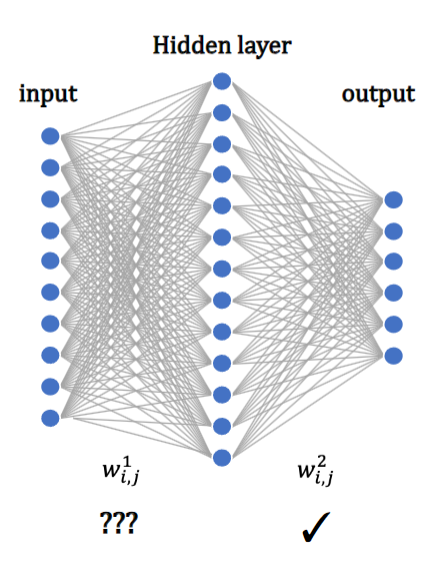
\includegraphics[width=0.3\linewidth]{creditassignment.png}
    \caption{Backpropogation}
    \label{fig:enter-label}
\end{figure}
Neural networks up until the 1970s were not very useful for two main reasons:
\begin{enumerate}
    \item Not clear how to train a NN of more than 1 layer (known as the \textbf{credit assignment problem})
    \item A neural network of only \textbf{one layer cannot describe complex functions}, two or more can represent any function (in theory with infinite width).
\end{enumerate}
\begin{definition}
    \textbf{Credit Assignment Problem:} the challenge of figuring out \textbf{how much each neuron in a network contributed to the final prediction or output}. It's about understanding which parts of the network were most \textbf{responsible for the outcome} and how changes in \textbf{individual neurons affect the overall performance}. 
\end{definition}

\begin{idea}
    Solving the credit assignment problem is essential for training neural networks effectively, as it allows us to identify which parts of the network \textbf{need adjustment or improvement}. Without a clear understanding of credit assignment, it's challenging to fine-tune networks, diagnose issues, and ensure consistent learning and performance improvement.
\end{idea}

The credit assignment problem was solved by \textbf{backpropagation}, a method that describes how to distribute errors to neurons \textbf{not adjacent to the output layer}.

\begin{definition}
    \textbf{Backpropagation}: a method in training neural networks, where the \textbf{network adjusts its internal parameters (weights and biases) by computing the gradient of the loss function} with respect to these parameters. This allows the network to learn and improve its predictions over time.
\end{definition}

Backpropagation uses a \textbf{dynamic programming}-like approach to calculate gradients and adjust weights in neural networks. The combination of \textbf{gradient descent} and \textbf{dynamic programming} is called backpropogation. It propagates error information \textbf{backward} through the layers, updating the weights in a way that \textbf{optimizes the network's performance over time.}  \\

\noindent\textbf{Multiple Layers with Non-Linearity}

\begin{figure}[h!t]
    \centering
    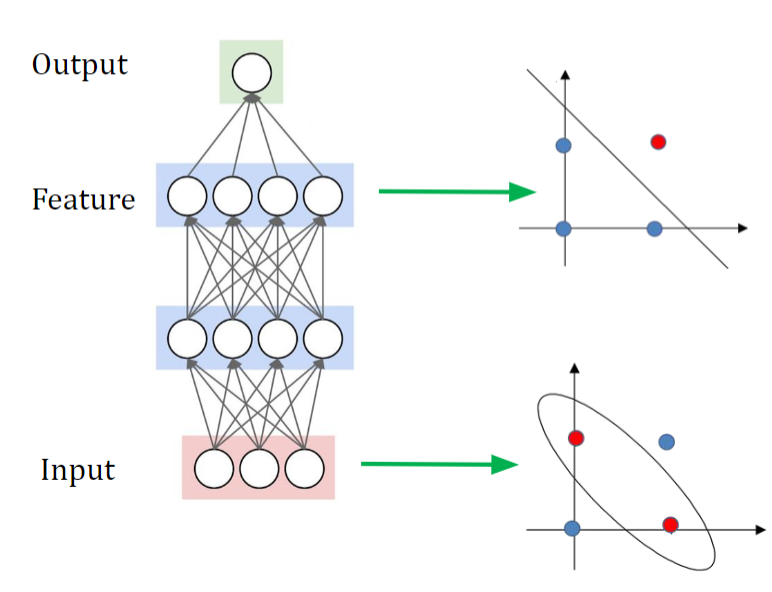
\includegraphics[width=0.4\linewidth]{multiplelayersnonlinearity.png}
    \caption{Multiple Layers with Non-Linearity}
    \label{fig:enter-label}
\end{figure}
\begin{itemize}
    \item Neural networks can be viewed as a way of learning features directly and end-to-end from raw input data.
    \item You can use the activations of the layer before the last layer as high-level features representing the input data.
    \item The goal being that the final layer is presented with a \textbf{linear separation}.
\end{itemize}

\begin{idea}
 Essentially, the network \textbf{maps (or projects) input, which is not linearly separable, to other dimensions (spaces) where it does become linearly separable}. The output layer is a linear layer because by the time the data reaches it, \textbf{it is already linearly separable}. In these hidden layers, the network learns features in the input data.
\end{idea}

\noindent\textbf{Neural Network Architecture}\\
An architecture of a neural network describes the neurons and their connectivity. Architecture selection will greatly affect model performance. It is an example of a very significant \textbf{inductive bias}.
\begin{definition}
\textbf{Feed-Forward Network:} information only flows forward from \textbf{one layer to a later layer}, from the input to the output \textbf{without any loops or cycles}. It's designed to make predictions or classifications based on the input data \textbf{without internal feedback connections}.
\end{definition}
\begin{definition}
\textbf{Fully-Connected Network:} neurons between adjacent layers are \textbf{fully connected}. Each neuron in a given layer is connected to every neuron in the subsequent layer. This creates a \textbf{dense} and \textbf{interconnected structure} that enables \textbf{information to flow freely} between all layers.
\end{definition}
\begin{definition}
\textbf{Number of Layers:} number of \textbf{hidden layers + output layer} (not including input "layer")
\end{definition}

\begin{figure}[h!t]
    \centering
    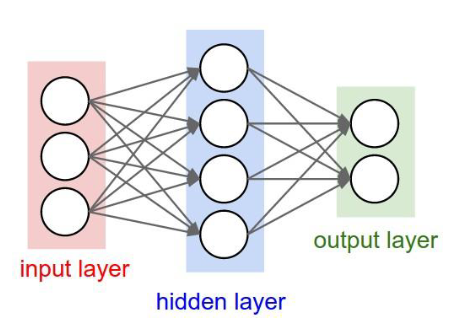
\includegraphics[width=0.3\linewidth]{twolayerNN.png}
    \caption{2-Layer Neural Network}
    \label{fig:enter-label}
\end{figure}
\begin{figure}[h!t]
    \centering
    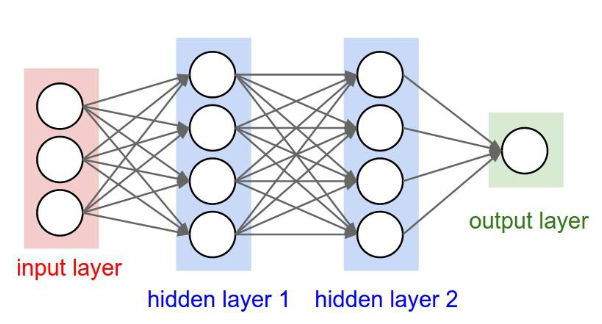
\includegraphics[width=0.325\linewidth]{threelayerNN.png}
    \caption{3-Layer Neural Network}
    \label{fig:enter-label}
\end{figure}

\begin{example}
    Given the code below, for a binary neural network classifier, answer the following questions.
    \begin{verbatim}
 def __init__ ( self ) :
     super ( MLP , self ) . __init__ ()
     self . firstLayer = nn . Linear (20 , 10)
     self . middleLayer = nn . Linear (10 , 10)
     self . lastLayer = nn . Linear (10 , 1)
 def forward ( self , input ) :
     activation1 = self . firstLayer ( input )
     activation1 = F . relu ( activation1 )
     activation2 = self . middleLayer ( activation1 )
     activation2 = F . relu ( activation2 )
     activation3 = self . middleLayer ( activation2 )
     activation3 = F . relu ( activation3 )
     activation4 = self . lastLayer ( activation3 )
     return activation4
    \end{verbatim}
\textbf{What is the input size of the network?:}
\\(20, B) Where B is the batch size.\\
\\\textbf{How many layers are there in the following network?:}
\\There are 4 layers in the network. Recall that the output layer is also considered a layer, while the input layer is not considered.\\
\textbf{\\What is the total number of parameters in the network (including biases)?:}
\\441 = (20*10 + 10) + (10*10 + 10) + (10*10 + 10) + (10*1 + 1)
\end{example}

\begin{idea}
    To calculate the \textbf{number of parameters} for a fully-connected network layer:
\[\text{Number of weights} = \text{Input size (entering layer) } \cdot \text{ Number of Neurons (in layer) } + \text{ Bias Term (for each neuron in layer)}\]
Only include bias term if it is assumed to exist.

\end{idea}

\begin{example}
    Calculating number of parameters (weights) for Fully-Connected Networks:
    \begin{itemize}
        \item Input: 200 x 200 pixels = 40000
        \item 1st hidden layer: 500 neurons
        \item 2nd hidden layer: 200 neurons
    \end{itemize}
(Weights = 40 000 x 500 + 500 x 200) + (Bias = 500 + 200) = 20100700 parameters
\end{example}

\begin{example}
    Calculating number of parameters (weights) for Fully-Connected Networks:
    \begin{itemize}
        \item self.fc1 = nn.Linear(16, 100)
        \item self.fc2 = nn.Linear(32, 100)
    \end{itemize}
(Weights = 16 x 100 + 32 x 100) + (Bias = 100 + 100) = 5000 parameters
\end{example}

\section{Hyperparameters}

While neural network \textbf{parameters}, such as weights, are updated through \textbf{Gradient Descent} \textbf{(Inner loop of optimization)}, \textbf{hyperparameters} are tuned by methods such as \textbf{Grid Search} and\textbf{ Random Search} \textbf{(Outer loop of optimization)}. Most of the time, \textbf{Random Search is all we need} as \textbf{Grid Search is very time consuming and costly}. 

\begin{figure}[h!t]
    \centering
    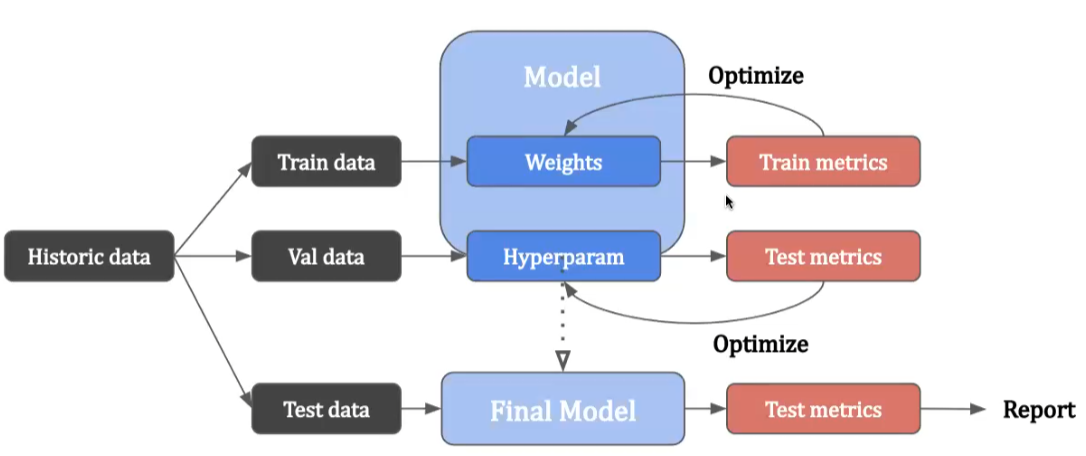
\includegraphics[width=0.75\linewidth]{hyperparams.png}
    \caption{How split data affects optimization}
    \label{fig:enter-label}
\end{figure}

\begin{figure} [h!t]
    \centering
    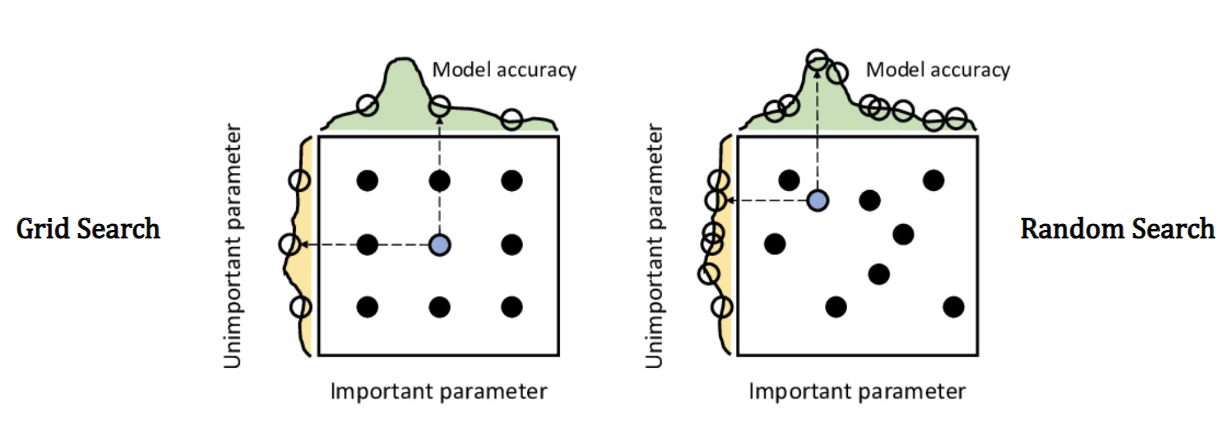
\includegraphics[width=0.75\linewidth]{tuninghyperparams.png}
    \caption{Grid Search and Random Search}
    \label{fig:enter-label}
\end{figure}

\begin{definition}
    \textbf{Grid Search:} involves creating a \textbf{predefined} grid of hyperparameter values to explore. It \textbf{exhaustively evaluates all possible combinations} of these values. It systematically searches through the entire parameter space, testing each combination to find the \textbf{best-performing set} of hyperparameters. Grid search is ideal when the hyperparameter space is relatively small and the interactions between hyperparameters are not too complex.
\end{definition}

\textbf{Pros of Grid Search}:

\begin{itemize}
    \item Exhaustive search that \textbf{guarantees optimal hyperparameters} within the specified search space.
    \item Systematic approach that \textbf{covers all combinations}.
\end{itemize}

\textbf{Cons of Grid Search}:

\begin{itemize}
    \item \textbf{Computationally expensive} when the search space is large.
    \item Inefficient when many \textbf{hyperparameters are not influential}.
\end{itemize}

\begin{definition}
    \textbf{Random Search:} \textbf{randomly} samples hyperparameters from a specified distribution or range. It performs a \textbf{certain number of random trials}, independently of each other, and evaluates the model's performance with each set of hyperparameters. Random search is particularly useful when the search space is large or when the impact of individual hyperparameters is less clear.\textbf{ Generally better than Grid Search}.
\end{definition}

\textbf{Pros of Random Search:}

\begin{itemize}
    \item More \textbf{efficient} when the search space is large or when some hyperparameters are less influential.
    \item \textbf{Less computationally demanding} compared to grid search for large search spaces.
\end{itemize}

\textbf{Cons of Random Search:}

\begin{itemize}
    \item There's no guarantee of finding the optimal hyperparameters, as it \textbf{relies on chance}.
    \item It might require more trials to converge to the best solution compared to grid search.
\end{itemize}

\section{Optimizers}

Defining a loss function turns a \textbf{learning problem into an optimization problem}. An optimizer determines, based on the value of the loss function, \textbf{how each parameter (weight) should change}. The optimizer solves the \textbf{credit assignment problem}. We assign credit to the parameters based on how the network performs by using optimizers that are based on \textbf{gradient descent}.\\

\noindent\textbf{Stochastic Gradient Descent (SGD)}

\begin{figure}[h!t]
    \centering
    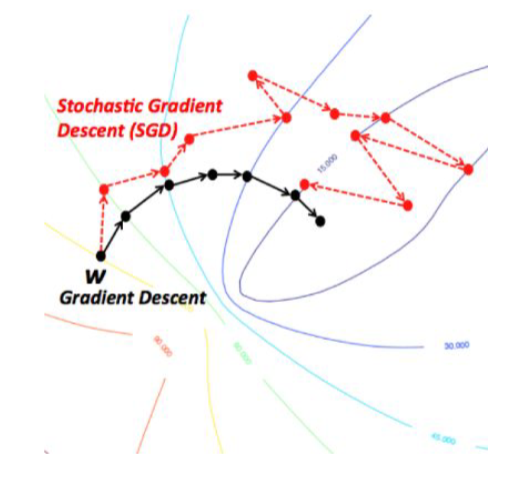
\includegraphics[width=0.35\linewidth]{SGD.png}
    \caption{Stochastic Gradient Descent}
    \label{fig:enter-label}
\end{figure}

\begin{itemize}
    \item For each iteration, evaluate a training sample from the dataset taken at random.
    \item Computing the gradient takes less time, but... may not actually be faster...
    \item Optimization path that looks rather erratic.
    \item SGD allows you to do more of a global search for an optimum, often resulting in a better set of weights for your model.
    \item Gradient Descent (GD) on the entire training data!
\end{itemize}

\begin{definition}
    \textbf{Stochastic Gradient Descent:} an optimization algorithm used to iteratively (\textbf{one at a time}) update the parameters of a model by computing the gradient of the loss function using a \textbf{randomly selected subset of the training data} in each iteration.
\end{definition}

\noindent\textbf{Mini-Batch Gradient Descent}

Instead of working with one sample at a time... can apply batching...
\begin{enumerate}
    \item Use our network to make predictions for $n$ samples
    \item Compute the average loss for those $n$ samples
    \item Take a “step” to optimize the average loss of those $n$ samples
\end{enumerate}

\begin{theorem}
    Set \textbf{batch size} close to \textbf{GPU memory} to use as much memory as possible!
\end{theorem}

\noindent\textbf{Batch size:} Number of training examples used per optimization “step”. \\
\noindent\textbf{Iteration:} One step - The parameters are updated once per iteration. \\
\textbf{Epoch:} Number of times all the training data is used once to update the parameters. \\
Suppose there are 1000 samples in the training data, if we set the batch size to 10, then 1 epoch will contain 100 iterations.

\begin{definition}
    \textbf{Mini-Batch Gradient Descent:} an optimization algorithm used to update the parameters of a model by computing the gradient of the loss function using a small subset (mini-batch) of the training data in each iteration, striking a \textbf{balance between the efficiency of Stochastic Gradient Descent (SGD) and the stability of Batch Gradient Descent}.
\end{definition}

\begin{warning}
    What happens when the \textbf{batch size is ineffective}?
    \begin{itemize}
        \item Too small:
        \begin{itemize}
            \item We optimize a (possibly very) different function loss at each iteration
            \item Noisy
        \end{itemize}
        \item Too large:
        \begin{itemize}
            \item Expensive
            \item Average loss might now change very much as batch size grows
            \item The true gradient is not always the best gradient for optimization; some
amount of noise in your gradients can help training (converge faster), so
larger batch size is not always better.
        \end{itemize}
    \end{itemize}
\end{warning}

A deep neural network has millions or billions of parameters.
Real gradient descent of a deep network is optimization in millions
of dimensions!
Most points of zero gradients are saddle points.
Plateaus are a problem but can be addressed using specialized
variants on gradient descent.\\

\noindent\textbf{Stochastic Gradient Descent (SGD) with Momentum}
\begin{figure}[h!t]
    \centering
    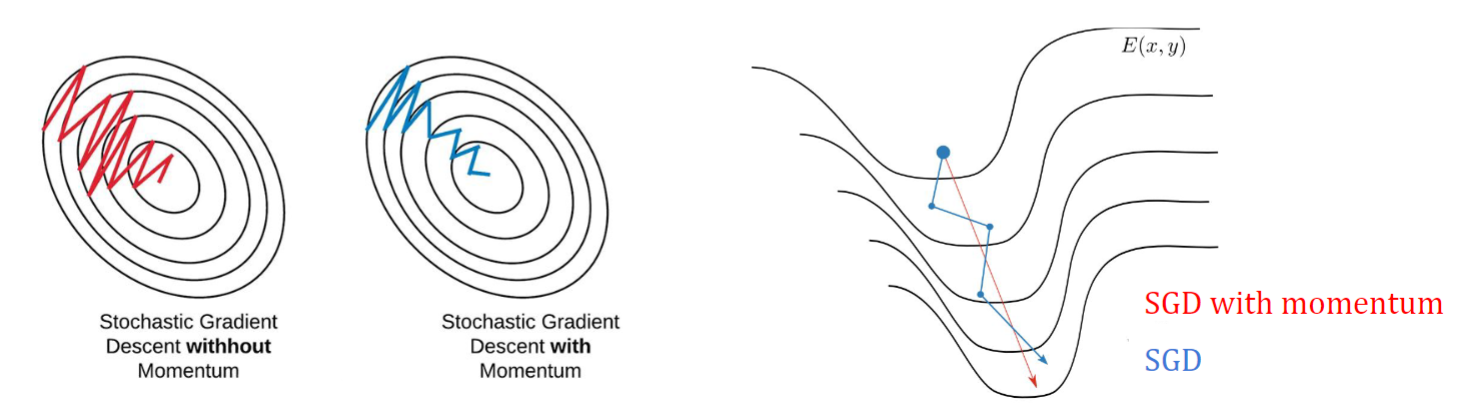
\includegraphics[width=0.7\linewidth]{SGDWM.png}
    \caption{SGD with Momentum}
    \label{fig:enter-label}
\end{figure}
\begin{definition}
    \textbf{Ravines:}  areas where the surface curves much more steeply in one dimension than in
another, common around local optima.
\end{definition}

\begin{itemize}
    \item SGD has trouble navigating ravines → it oscillates across the slopes of the ravine.
    \item Momentum helps accelerate SGD in the relevant direction and dampens oscillations.
    \item The momentum term increases for dimensions whose gradients point in the same directions and reduces updates for dimensions whose gradients change directions
    \item Analogy → we push a ball down a hill. The ball accumulates momentum as it rolls downhill, becoming faster and faster on the way until it reaches its terminal velocity

\end{itemize}

\begin{definition}
    \textbf{Stochastic Gradient Descent with Momentum:} an optimization algorithm used to iteratively update the parameters of a model by incorporating a moving average of past gradients. This momentum term helps accelerate the convergence process by reducing oscillations and smoothing out the optimization path, leading to faster and more stable convergence.
\end{definition}


\[v_{t+1} = \mu v_{t} - \alpha \nabla J(\theta_t)\]


\[\theta_{t+1} = \theta_t + v_{t+1}\]



Where:
\begin{itemize}
  \item $v_{t+1}$: Updated velocity at time step $t+1$
  \item $\mu$: Momentum coefficient (typically between 0 and 1)
  \item $v_{t}$: Velocity at time step $t$
  \item $\alpha$: Learning rate
  \item $\nabla J(\theta_t)$: Gradient of the cost (loss) function $J$ with respect to the parameters $\theta$ at time step $t$
  \item $\theta_{t+1}$: Updated parameters at time step $t+1$
  \item $\theta_t$: Parameters at time step $t$
\end{itemize}


\noindent\textbf{Adaptive Moment Estimation (Adam)}

\begin{figure}[h!t]
    \centering
    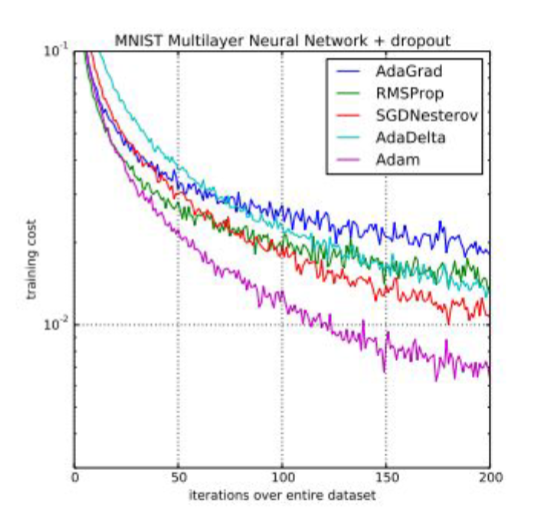
\includegraphics[width=0.4\linewidth]{optimizers.png}
    \caption{Optimizers relative to each other in terms of training cost over iterations}
    \label{fig:enter-label}
\end{figure}

\begin{definition}
    \textbf{Adaptive Moment Estimation:} a popular optimization algorithm used for tuning the parameters of a model during training. It combines concepts from both Adaptive Gradient Algorithm (AdaGrad) and Root Mean Square Propagation (RMSProp) to adaptively adjust learning rates for each parameter. This helps achieve efficient and stable convergence by individually adapting the learning rates while also incorporating momentum-based updates.
\end{definition}

\begin{itemize}
    \item Adaptive learning rates → each weight has its own rate
    \item Incorporates momentum and adaptive learning rate:
    \begin{itemize}
        \item rapid convergence
        \item requires minimal tuning
        \item commonly used optimizer
    \end{itemize}
\end{itemize}

\begin{figure}[h!t]
    \centering
    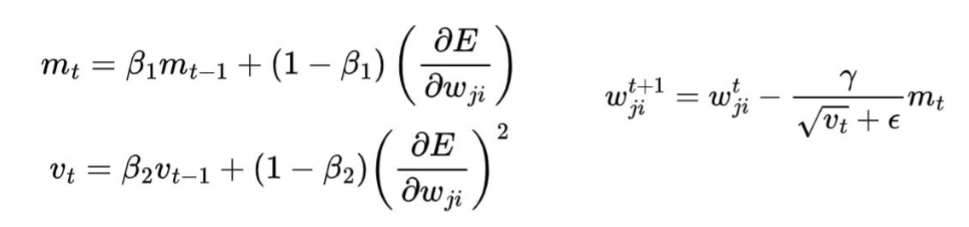
\includegraphics[width=0.4\linewidth]{adam.png}
    \caption{Adam Optimizer Equations}
    \label{fig:enter-label}
\end{figure}

\begin{idea}
    \textbf{Optimizer Summary:}\\

    1. \textbf{SGD (Stochastic Gradient Descent)}:
   \begin{itemize}
       \item \textbf{Use when:} Training on large datasets with limited computational resources.
       \item \textbf{Scenario:} Updates model parameters using the gradient of a single randomly selected data point.
       \item \textbf{Pros:} Faster updates, can escape local minima, suitable for online learning.
       \item \textbf{Cons:} Noisy updates, slower convergence on some problems.
   \end{itemize}

2. \textbf{SGD with Momentum}:
   \begin{itemize}
       \item \textbf{Use when:} Training needs faster convergence and better handling of noisy gradients.
       \item \textbf{Scenario:} Incorporates a moving average of past gradients to accelerate convergence.
       \item \textbf{Pros:} Faster convergence, reduced oscillations, better handling of noisy data.
       \item \textbf{Cons:} May overshoot in some cases.
   \end{itemize}

3. \textbf{Adam (Adaptive Moment Estimation)}:
   \begin{itemize}
       \item \textbf{Use when:} Training deep neural networks with diverse architectures.
       \item \textbf{Scenario:} Combines adaptive learning rates for each parameter and momentum-like behavior.
       \item \textbf{Pros:} Fast convergence, adaptive learning rates, well-suited for complex models.
       \item \textbf{Cons:} Can require tuning, memory-intensive.
   \end{itemize}

4. \textbf{Mini Batch Gradient Descent}:
   \begin{itemize}
       \item \textbf{Use when:} Training on medium to large datasets efficiently.
       \item \textbf{Scenario:} Computes gradient on a small subset (mini-batch) of data.
       \item \textbf{Pros:} Faster convergence than pure SGD, benefits from vectorized operations.
       \item \textbf{Cons:} Batch size selection matters, noise in updates, needs more memory.
   \end{itemize}
\end{idea}


\section{Learning Rate}

The learning rate determines the \textbf{size of the step} that an optimizer takes during each iteration. Larger step size means a bigger change in the parameters (weights) in each iteration.

\begin{figure}[h!t]
    \centering
    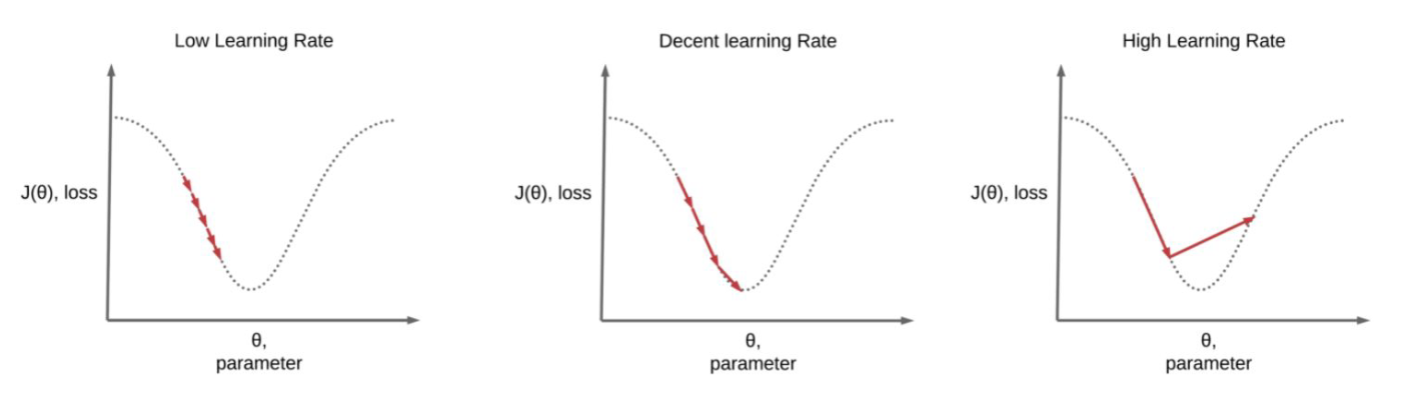
\includegraphics[width=0.8\linewidth]{learningrate.png}
    \caption{Learning Rate Size}
    \label{fig:enter-label}
\end{figure}

\begin{warning}
    What happens when the \textbf{learning rate size is ineffective}?
    \begin{itemize}
        \item Too small:
        \begin{itemize}
            \item Very small parameter change
            \item Longer training time
        \end{itemize}
        \item Too large:
        \begin{itemize}
            \item Noisy
            \item Detrimental to training
        \end{itemize}
    \end{itemize}
\end{warning}

\begin{figure}[h!t]
    \centering
    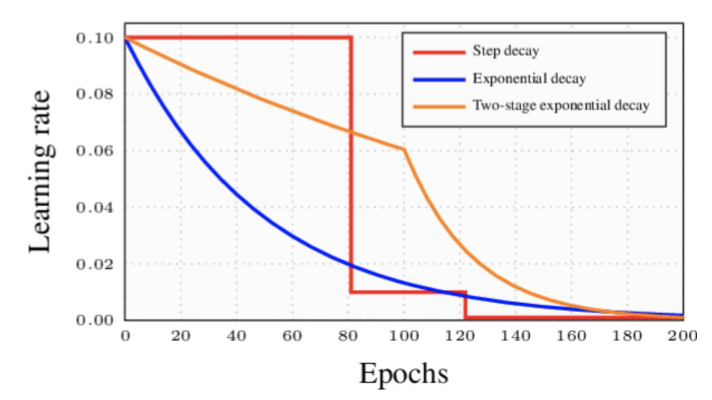
\includegraphics[width=0.5\linewidth]{learningrateoverepochs.png}
    \caption{How learning rate changes over epochs}
    \label{fig:enter-label}
\end{figure}

\textbf{The appropriate learning rate depends on:}
\begin{itemize}
    \item The learning problem
    \item The optimizer
    \item The batch size
    \begin{itemize}
        \item \textbf{Large batch}: larger learning rates
        \item \textbf{Small batch}: smaller learning rates
    \end{itemize}
    \item The stage of training
    \begin{itemize}
        \item Reduces as training progresses
    \end{itemize}
\end{itemize}

\section{Normalization}

\begin{definition}
   \textbf{Normalization:} refers to the process of \textbf{scaling and shifting} input data or intermediate activations to ensure that they have a \textbf{consistent and suitable range}. This aids in improving the stability and convergence of training by mitigating issues related to varying magnitudes of data across features or layers.
\end{definition}
We always normalize the inputs to prevent the model from paying attention to the features with larger range.

\[X_i = \frac{X_i - \mu_i}{\sigma_i}\]

Where:
\begin{itemize}
  \item $X_i$ is the original value of the $i$th element in the data vector.
  \item $\mu_i$ is the mean (average) of all $i$th elements across a batch of data.
  \item $\sigma_i$ is the standard deviation of all $i$th elements across the same batch of data.
\end{itemize}

\begin{figure}[h!t]
    \centering
    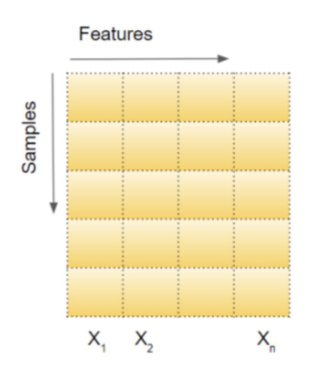
\includegraphics[width=0.3\linewidth]{normalization.png}
    \caption{Normalization}
    \label{fig:enter-label}
\end{figure}
\begin{itemize}
    \item However, this only normalizes data for the first layer. How do we normalize activations of each layer for the next layer?
\end{itemize}

\noindent\textbf{Batch Normalization}

\begin{definition}
    \textbf{Batch Normalization:} a technique used to normalize the activations of a layer by adjusting them to have zero mean and unit variance across a mini-batch of training examples. This improves training stability, speeds up convergence, and enables higher learning rates by reducing the internal covariate shift problem.
\end{definition}

\begin{theorem}
    \textbf{Internal Covariate Shift Problem:}  the change in the distribution of the input to a given layer during training. As the network learns and its parameters get updated, the distribution of activations in each layer may shift, making the optimization process more difficult. This can slow down training and require the use of lower learning rates to prevent the network from diverging or getting stuck.
\end{theorem}

Batch normalization essentially combats the internal covariate shift problem by normalizing the inputs of each layer within a mini-batch during training.

\begin{figure}[h!t]
    \centering
    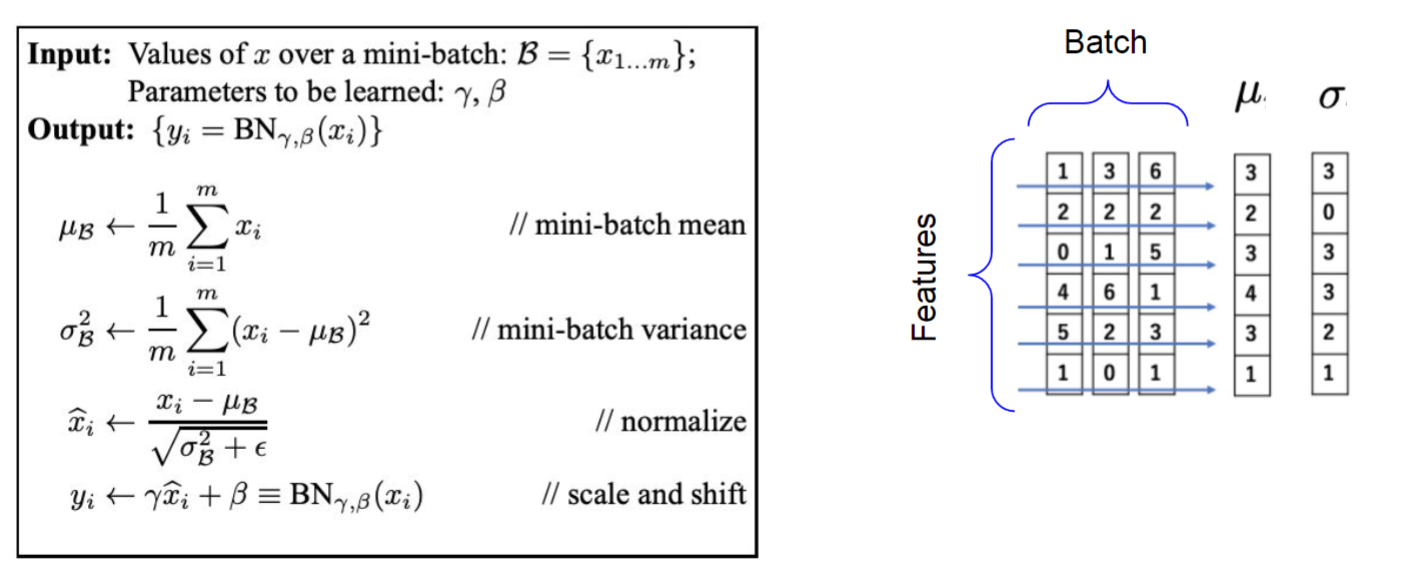
\includegraphics[width=0.75\linewidth]{batchnormalization.png}
    \caption{Batch Normalization}
    \label{fig:enter-label}
\end{figure}

\begin{definition}
    \textbf{Inference Time:} refers to the phase when a trained machine learning model is applied to new, unseen data to make predictions or produce outputs based on the knowledge it gained during its training phase.
\end{definition}

Batch Normalization primarily affects the \textbf{training phase} of a neural network, and its operation during inference time differs slightly from its behavior during training. During training, Batch Normalization computes the mean and standard deviation of each feature within a mini-batch of data, normalizes the features, and then scales and shifts them based on learnable parameters. These normalization statistics can change from one batch to another, helping with faster convergence and better generalization.\\

However, during inference time, the model processes individual examples or small batches of examples one at a time, rather than in the larger training batches. This raises the question of how to handle the normalization statistics, as there is no longer a batch of data to compute them from.\\

A way to solve this issue is \textbf{Moving Average}. 

\begin{definition}
    \textbf{Moving Average:} addresses the challenge of Batch Normalization during inference by maintaining running statistics, including the\textbf{ mean} and \textbf{standard deviation} of features, over the course of training. These running statistics are computed by \textbf{aggregating the statistics from all training batches}. During inference, these \textbf{accumulated statistics are used to normalize the input features}, providing a consistent behavior that aligns with the model's learned behavior during training. This method helps ensure that the benefits of Batch Normalization are retained when making predictions on new data while avoiding the need to compute statistics on small inference batches.
\end{definition}

\begin{figure}[h!t]
    \centering
    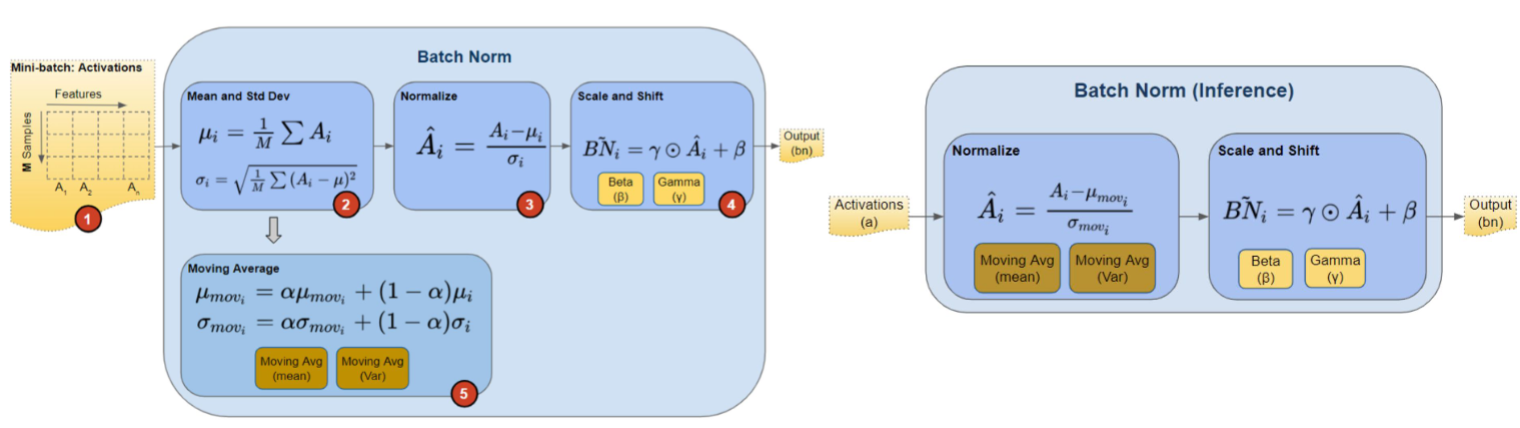
\includegraphics[width=1\linewidth]{batchnormalizationinference.png}
    \caption{Inference Time}
    \label{fig:enter-label}
\end{figure}

\noindent\textbf{Pros:}
\begin{itemize}
\item Higher learning rate $\rightarrow$ speeding up the training
\item Regularizes the model
\item Less sensitivity to initialization
\end{itemize}
\textbf{Cons:}
\begin{itemize}
\item Depends on batch size $\rightarrow$ No effect with small batches
\item Cannot work with SGD\\
\end{itemize}

\begin{warning}
    If the batch size is 1, we cannot use batch normalization!
\end{warning}

\noindent\textbf{Layer Normalization}

\begin{definition}
    \textbf{Layer Normalization:} a technique used to normalize the activations of a layer across the entire batch, focusing on the mean and standard deviation of each feature independently. This helps stabilize training, improve convergence, and reduce sensitivity to weight initialization, enhancing the network's performance.
\end{definition}

\begin{figure}[h!t]
    \centering
    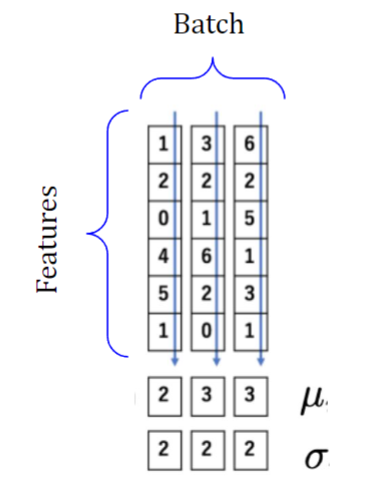
\includegraphics[width=0.25\linewidth]{layernorm.png}
    \caption{Layer Normalization}
    \label{fig:enter-label}
\end{figure}

\begin{itemize}
    \item Normalization is applied on the neuron for a single instance across all features
    \item Simpler to implement, no moving averages or parameters
    \item Not dependent on batch size
    \item Works on par with batch normalization or even better
\end{itemize}

\section{Regularization}

\begin{definition}
    \textbf{Regularization:} refers to techniques that mitigate overfitting by adding constraints or penalties to the model's training process. These techniques discourage the model from fitting noise in the training data and encourage it to learn more generalizable patterns, ultimately enhancing its ability to perform well on unseen data. Essentially, \textbf{techniques that make it hard for the model to memorize.}
\end{definition}

\textbf{Dropout}

\begin{definition}
    \textbf{Dropout:}  involves randomly \textbf{deactivating} (dropping out) \textbf{a proportion of neurons} during each training iteration. This helps prevent overfitting by encouraging the network to learn more robust and independent features, improving its generalization on new data.
\end{definition}

\begin{figure}[h!t]
    \centering
    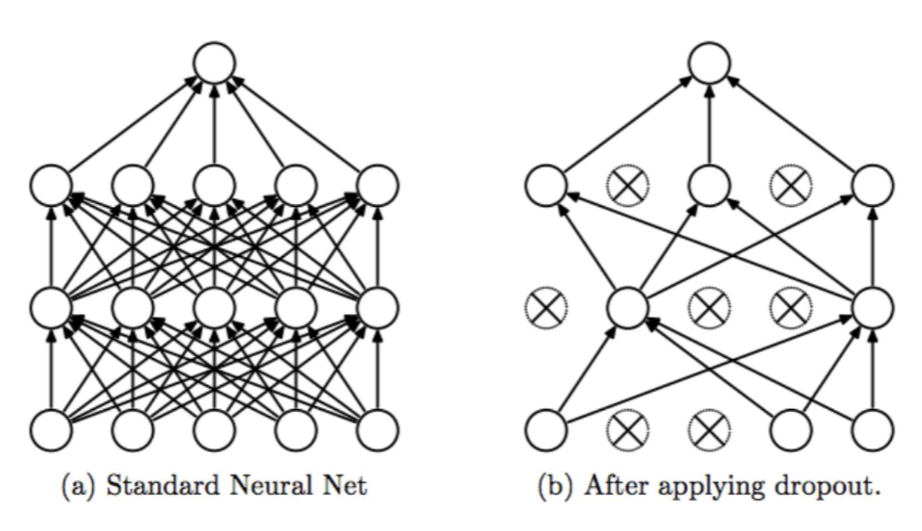
\includegraphics[width=0.5\linewidth]{dropout.png}
    \caption{Dropout}
    \label{fig:enter-label}
\end{figure}
\begin{itemize}
    \item Forces a neural network to learn more robust features by forcing to learn the \textbf{underlying distribution} of the data rather than memorizing it
    \item A very \textbf{straightforward} and \textbf{efficient} way to regularize deep models
    \item During training → Drop activations (set to 0) with probability p
    \begin{itemize}
        \item Implementation wise, neurons are muliplied by 0 to drop, and 1 to be kept
    \end{itemize}
    \item During inference → multiply weights by (1-p) to keep the same distribution
\end{itemize}

\noindent\textbf{Weight Decay (L2)}
\begin{definition}
    \textbf{Weight Decay (L2):} a technique that involves adding a \textbf{penalty term (summation of all weights of the network) to the loss function} during training. This penalty discourages the model from assigning excessively large weights to its parameters, promoting simpler and more generalizable solutions, which reduces the risk of overfitting.
\end{definition}

\begin{figure}[h!t]
    \centering
    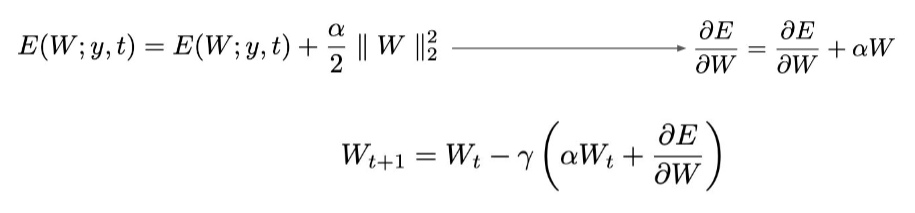
\includegraphics[width=0.75\linewidth]{weightdecay.png}
    \caption{Weight Decay}
    \label{fig:enter-label}
\end{figure}

\begin{itemize}
    \item When a model "wants" to overfit or memorize, it tends to \textbf{inflate} weights, which causes the space to be warped in a strange way, leading to memorization
    \item Prevents the weights from growing too much → Lowering variance
    \item Weight reduction is multiplicative and proportion to the scale of W
\end{itemize}

\noindent\textbf{Early Stopping with Patience}
\begin{definition}
    \textbf{Early Stopping with Patience:} refers to \textbf{monitoring} the model's performance on a validation set during training and \textbf{halting} the training process when the performance stops improving for a certain number of consecutive epochs (patience). This technique prevents overfitting by selecting a model that achieves good validation performance before it starts to degrade due to excessive training.
\end{definition}

\begin{figure}[h!t]
    \centering
    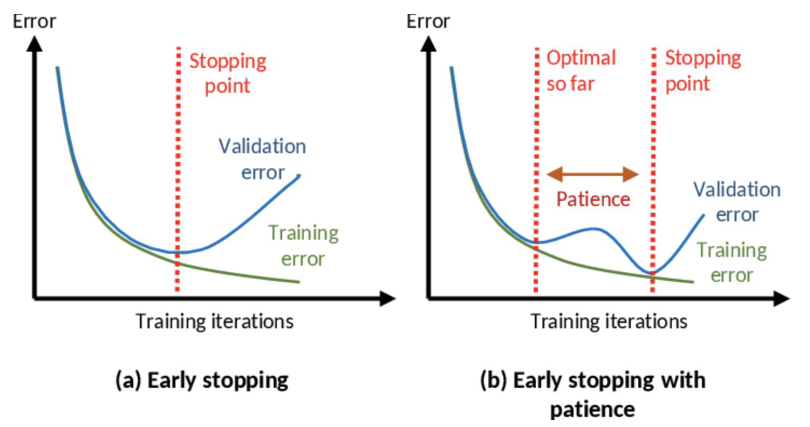
\includegraphics[width=0.75\linewidth]{earlystopping.png}
    \caption{Early Stopping with Patience}
    \label{fig:enter-label}
\end{figure}

\begin{itemize}
    \item In each training iteration observe the validation loss
    \item As soon as validation loss starts to increase, start a counter
    \item If the validation loss decreases, reset the counter
    \item Otherwise, wait for a fixed iterations (patience) and then stop the training
\end{itemize}

\section{Evaluation and Debugging}
\textbf{Debugging Tips}
\begin{itemize}
    \item Make sure your model \textbf{can overfit}
    \begin{itemize}
        \item Make sure you can get loss to decrease w.r.t training data
        \item If model cannot even learn the training data, it's not going to be able to predict validation or test data
    \end{itemize}
    \item Make sure that your network is training: i.e. loss is going down.
    \begin{itemize}
        \item Sanity check!
    \end{itemize}
    \item Ensures that you are using the right variable names, and rule out other programming bugs that are difficult to discern from architecture issues.
    \item Confusion Matrix
    \begin{itemize}
        \item True Positive (TP), False Positive (FP), True Negative (TN), False Negative (FN)
    \end{itemize}
    \item 2D Projections of Data (visualizing class clusters)
    \begin{itemize}
        \item PCA, t-SNE
    \end{itemize}
\end{itemize}

\noindent\textbf{Confusion Matrix}

\begin{definition}
    \textbf{Confusion Matrix:} tabular representation used to display the performance of a classification model. It summarizes the predicted class labels against the actual class labels, showing counts of true positive, true negative, false positive, and false negative predictions.
\end{definition}

\begin{figure}[h]
    \centering
    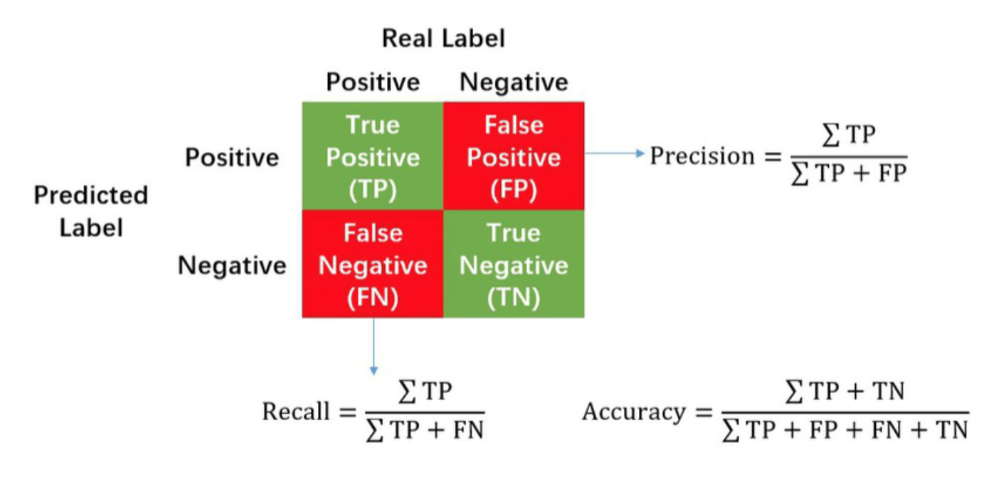
\includegraphics[width=0.7\linewidth]{confusionmatrix.png}
    \caption{Confusion Matrix}
    \label{fig:enter-label}
\end{figure}

\begin{warning}
    \textbf{Accuracy} is only valid when class distributions are equal (\textbf{balanced dataset})! \textbf{F1 Score} should be used in cases where the \textbf{dataset is unbalanced}.
\end{warning}

\begin{figure}[h!t]
    \centering
    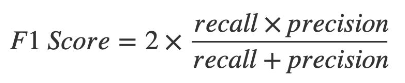
\includegraphics[width=0.45\linewidth]{f1.png}
    \caption{F1 Score}
    \label{fig:enter-label}
\end{figure}

\begin{figure}[h!t]
    \centering
    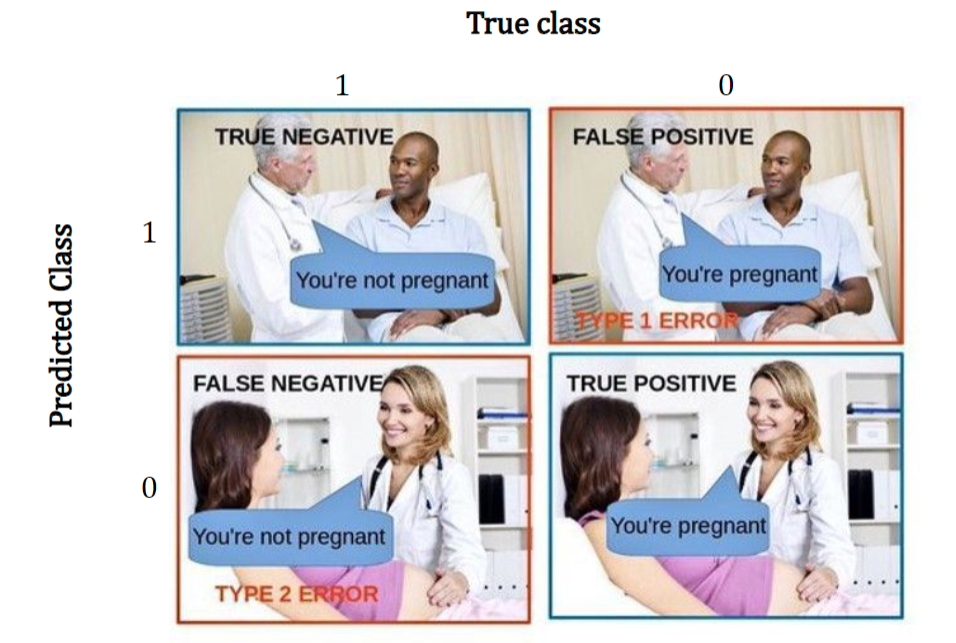
\includegraphics[width=0.5\linewidth]{ConfusionMatrixEx.png}
    \caption{Confusion Matrix Example}
    \label{fig:enter-label}
\end{figure}


\newpage

\textbf{MNIST 2D Visualization}

\begin{figure}[h!t]
    \centering
    \includegraphics[width=0.4\linewidth]{2ddatavis.png}
    \caption{t-SNE for 2D projection and
visualization of data structure}
    \label{fig:enter-label}
\end{figure}

\begin{idea}
    Data that appears neatly clustered in groups by class indicates a \textbf{well-performing model}.
\end{idea}
\chapter{Convolutional Neural Networks (CNNs)}

\space

\section{Motivation}

\textbf{Fully connected networks become useless when the dataset is not nicely preprocessed, centered, etc}. When the size of the input is incompatible with the dimensions of the model, the fully connected will no longer work because it needs to be retrained.\\

\\\textbf{Using a large fully connected network has some downsides}:
\begin{itemize}
    \item \textbf{Computation complexity (exponentially) grows} $\rightarrow$ harder to train
    \item \textbf{Larger capacity} $\rightarrow$ more data to generalize
    \item \textbf{Bad inductive bias} $\rightarrow$ Ignores geometry of image data (relative distances between objects in an image)
    \begin{itemize}
        \item Recall that in fully connected networks, the pixels of an image are stacked to make a line of pixels (1D) instead of a 2D image
    \end{itemize}
    \item \textbf{Not flexible} $\rightarrow$ Different image sizes require different models
    \begin{itemize}
        \item When we want to put a new image size as input in a model, we need to train the model from scratch
    \end{itemize}
\end{itemize}

\section{Convolution Operator}

\begin{definition}
    \textbf{Convolution:} Convolution is a mathematical operation on two functions f and g that expresses how
the shape of one is modified by the other. The function f is the input function and the function g is known as the\textbf{ kernel}.

\[
(f * g)(t) = \sum_{\tau = -\infty}^{\infty} f(\tau) \cdot g(t - \tau)
\]

\end{definition}

\begin{figure} [h!t]
    \centering
    \includegraphics[width=0.27\linewidth]{convolution.png}
    \caption{Convolution}
    \label{fig:enter-label}
\end{figure}

\section{Convolution in 2D for Images}

To apply the convolutional operator to 2D space, we simply \textbf{add another dimension} to the equation.\\

\\\textbf{Convolution of Image \( I \) with filter kernel \( K \):}
\begin{enumerate}
    \item Multiply each pixel in the range of the kernel by the corresponding element of the kernel.
    \item Sum all these products and write the result to a new 2D array.
    \item Slide the kernel across all areas of the image until you reach the image's edges.
    \item Once the edge is reached, go back horizontally to the start but slide down one pixel
\end{enumerate}


\[y[m,n] = I[m,n] * K[m,n = \sum_{j=-\infty}^{\infty} \sum_{j=-\infty}^{\infty} I[i,j]\cdot K[m-i, n-j]\] 
\begin{figure}[h!t]
    \centering
    \includegraphics[width=0.5\linewidth]{convex1.png}
    \caption{Step 1}
    \label{fig:enter-label}
\end{figure}

\begin{figure}[h!t]
    \centering
    \includegraphics[width=0.525\linewidth]{convex2.png}
    \caption{Step 2}
    \label{fig:enter-label}
\end{figure}

\begin{idea}
    Convolution of an image is applying a kernel to the image while sliding the kernel across the image
\end{idea}


\textbf{Why use convolution?}
\begin{itemize}
    \item In signal processing, convolution is used to \textbf{extract important features} of the input signal
    \item Instead of trying to make prediction directly on image pixels, such as what we've done in fully connected networks, we are applying a kernel to the image pixels to extract interesting features, then do predictions based on those features (which are the most important assets of the image)
    \item The output of the kernel applied to the image is the most important assets of the image extracted by the kernel\\
\end{itemize}

\begin{definition}
    \textbf{Kernel:} a kernel, also known as a filter, is a small matrix used to extract specific features from an input image or data. It's applied through the process of convolution to scan the input and produce feature maps that highlight particular patterns, such as edges, textures, or other relevant characteristics. 
\end{definition}

\noindent\textbf{Examples of kernels (filters) applied to images}

\begin{itemize}
    \item \textbf{Blurring:} averages out pixel intensities in an image
    \begin{figure}[h!t]
        \centering
        \includegraphics[width=0.45\linewidth]{blurringkernel.png}
        \caption{Blurring Filter}
        \label{fig:enter-label}
    \end{figure}
    \item \textbf{Vertical Edge Detector}
\begin{figure}[h!t]
    \centering
    \includegraphics[width=0.45\linewidth]{verticaledgekernel.png}
    \caption{Vertical Edge Detector}
    \label{fig:enter-label}
\end{figure}
    \item \textbf{Horizontal Edge Detector}
\begin{figure}[h!t]
    \centering
    \includegraphics[width=0.45\linewidth]{horizontaledgekernel.png}
    \caption{Horizonal Edge Detector}
    \label{fig:enter-label}
\end{figure}
    \item \textbf{Blob Detector:} detect regions that differ in properties, such as brightness or color, compared to
surrounding regions
\begin{figure}[h!t]
    \centering
    \includegraphics[width=0.45\linewidth]{blobdetectorkernel.png}
    \caption{Blob Detector}
    \label{fig:enter-label}
\end{figure}
\end{itemize}

\textbf{Where do these kernels come from?}

\begin{itemize}
    \item Before deep learning, people would spend years coming up with these kernels (hand-crafted)
    \item Classic computer vision used multi-stage feature (kernel) engineering
\end{itemize}

\begin{figure}[h!t]
    \centering
    \includegraphics[width=0.5\linewidth]{multistagekerneleng.png}
    \caption{Multi-stage feature (kernel) engineering of a licence plate recognition system}
    \label{fig:enter-label}
\end{figure}

\begin{itemize}
    \item There were two main problems with this method:
    \begin{enumerate}
        \item If one step fails, the subsequent steps wil also fail
        \item Hand-written algorithms don't work in real world scenarios due to fringe cases
    \end{enumerate}
\end{itemize}
\begin{itemize}
    \item This is where convolutional neural networks become useful
\end{itemize}

\section{Convolutional Neural Networks}

\begin{definition}
    \textbf{Convolutional Neural Network:} a type of deep learning model specifically designed for processing and analyzing grid-like data, such as images and sequences. It uses layers of learnable filters (kernels) to perform convolutions on the input data, enabling the network to automatically learn and extract hierarchical features. CNNs are highly effective for tasks like image recognition, object detection, and image generation due to their ability to capture local patterns and spatial relationships within the data.
\end{definition}

Convolutional neural networks were\textbf{ inspired by the Hubel and Wiesel Cat Experiments (1958-1959)}:
\begin{itemize}
    \item Individual neurons respond to stimuli only in a restricted region of the visual field
known as the \textbf{Receptive Field}.
\item Collection of such fields overlap to cover the entire visual area
\item Some neurons react only to images of horizontal lines, while others react line
orientations
\item Higher-level neurons are based on the outputs of neighbouring lower-level
neurons


\end{itemize}

\textbf{Introduce convolutional filters into neural networks so that we don’t have to hand
craft the features!}
\begin{itemize}
    \item \textbf{Locally connected layers}: local features in small regions of the image
    \item \textbf{Weight sharing:} detect the same local features across the entire image
    \item Neural Network \textbf{learns the kernel values} (or weights)
    \item More efficient than fully-connected networks since \textbf{outputs of kernels are connected to neurons} instead of each individual pixel of an image (weight sharing). 
    \item \textbf{Detecting:} the output (activation) is high if the feature is present
    \item \textbf{Feature:} something in the image, like an edge, blob, or shape
    

\end{itemize}

\begin{figure}[h!t]
    \centering
    \includegraphics[width=0.3\linewidth]{weightsharing.png}
    \caption{Weight Sharing}
    \label{fig:enter-label}
\end{figure}



\begin{figure}[h!t]
    \centering
    \includegraphics[width=0.5\linewidth]{fcvsconv.png}
    \caption{Fully Connected vs. Convolutional}
    \label{fig:enter-label}
\end{figure}

\newpage

While fully-connected networks require us to preprocess the input,

\begin{figure}[h!t]
    \centering
    \includegraphics[width=0.35\linewidth]{fc.png}
    \caption{Fully connected network}
    \label{fig:enter-label}
\end{figure}

convolutional neural networks apply convolution to image tensors and allow the network to learn and extract important low and high level features.

\begin{figure}[h!t]
    \centering
    \includegraphics[width=0.5\linewidth]{endtoend.png}
    \caption{End-to-end network}
    \label{fig:enter-label}
\end{figure}

Thus, in a model that uses both fully connected and convolutional layers, the \textbf{CNN part is the encoder} and the \textbf{FC part is the classifier}. The CNN part extracts features, which are passed to the FC part that classifies the input. \\

\begin{idea}
    Because everything is \textbf{jointly connected, the weights} of the convolutional and fully connected layers are \textbf{jointly optimized} according to the loss function. This means that the \textbf{end-to-end} network is not going to face the same problem as the multi-stage algorithm described earlier.
\end{idea}

\textbf{The numbers in the kernel are learned through gradient descent.} \\

\textbf{Forward and Backward Pass (kernels):}
\begin{itemize}
    \item Initialize the kernels randomly
    \item In forward pass, convolve the image with the kernel
    \item In backward pass, update the kernel using gradients
\end{itemize}

\begin{figure}[h!t]
    \centering
    \includegraphics[width=0.5\linewidth]{forwardbackwardpass.png}
    \caption{Kernel as a matrix of weights}
    \label{fig:enter-label}
\end{figure}
\textbf{General CNN Terminology:}

\begin{definition}
    \textbf{Zero Padding:} adding zeros around the border of the image before convolution.
\end{definition}

\begin{figure}[h!t]
    \centering
    \includegraphics[width=0.75\linewidth]{zeropadding.png}
    \caption{Zero Padding}
    \label{fig:enter-label}
\end{figure}

\textbf{Zero padding is applied for two main reasons:}
\begin{enumerate}
    \item Keep width and height consistent with the previous layer
    \item Keep the information around the border of the image
\end{enumerate}

\begin{definition}
    \textbf{Stride:}  distance between two consecutive positions of the kernel.
\end{definition}

\begin{figure}[h!t]
    \centering
    \includegraphics[width=0.75\linewidth]{stride.png}
    \caption{Stride}
    \label{fig:enter-label}
\end{figure}

Stride allows us to control the \textbf{output resolution}.

\begin{definition}
    \textbf{Feature Map:} a 2D or 3D array of values that represents the activations of specific features detected within an input data volume, generated by applying filters through convolutional operations in neural networks, particularly in convolutional neural networks (CNNs).
\end{definition}

\begin{theorem}
    \textbf{Computing the output size of the feature map (from convolving an image with a kernel)}\\

For each dimension of an input image with:
\begin{itemize}
    \item Image dimension of size \textbf{i}
    \item Kernel of size \textbf{k}
    \item Padding of size \textbf{p}
    \item Stride of size \textbf{s}
\end{itemize}
The size of output dimension is computed by:


\[o = [\frac{i + 2p - k}{s}] + 1\]
\\This equation assumes the kernel and image sizes are square!\\

\textbf{In the case that the sizes are not square}: 
    \begin{itemize}
        \item Image dimension of size \textbf{i x j}
        \item Kernel of size \textbf{k x l}
        \item Padding of size \textbf{p}
        \item Stride of size \textbf{s}
    \end{itemize}

We need to calculate the output of each dimension separately:

\[o_1 = [\frac{i + 2p - k}{s}] + 1\]
\[o_2 = [\frac{j + 2p - l}{s}] + 1\]
\end{theorem}

\begin{figure}[h!t]
    \centering
    \includegraphics[width=0.8\linewidth]{convout1.png}
    \caption{Output Calculation Example 1}
    \label{fig:enter-label}
\end{figure}

\begin{figure}[h!t]
    \centering
    \includegraphics[width=0.8\linewidth]{outconv2.png}
    \caption{Output Calculation Example 2}
    \label{fig:enter-label}
\end{figure}

\begin{figure}[h!t]
    \centering
    \includegraphics[width=0.8\linewidth]{outconv3.png}
        \caption{Output Calculation Example 3}
    \label{fig:enter-label}
\end{figure}

\newpage

\section{Convolution in 3D for RGB input}

In 3D, the kernel becomes a \textbf{3D tensor.}

\begin{figure}[h!t]
    \centering
    \includegraphics[width=0.5\linewidth]{conv3D.png}
    \caption{Convolution in 3D (RGB)}
    \label{fig:enter-label}
\end{figure}

\begin{example}
    \textbf{Calculating the number of trainable weights from an RGB input image and a convolution kernel}

    \begin{itemize}
        \item Colored input image: 3×28×28
        \item Convolution kernel: 3×3×3
    \end{itemize}

    The dimension of the kernel is 3 x 3 x 3, therefore there are \(3 x 3 x 3 = 27\) trainable weights.

\end{example}

\noindent\textbf{Expanding Feature Maps}

If we just use \textbf{one convolution, or one kernel, we are only able to detect one type of feature}, which isn't enough for information-rich images. The solution is to apply \textbf{multiple kernels at the same time to the image in parallel}, which will each extract a different feature, allowing for more than one feature to be extracted at a time. \\

\noindent Each kernel will produce an output, and these outputs will be stacked on top of each other to form the depths of the output.

\begin{figure}[h!t]
    \centering
    \includegraphics[width=0.5\linewidth]{expandingfeaturemaps.png}
    \caption{Applying multiple kernels}
    \label{fig:enter-label}
\end{figure}

\begin{theorem}
    The depths of the output = Number of kernels
\end{theorem}

\begin{figure}[h!t]
    \centering
    \includegraphics[width=0.75\linewidth]{examplemultiplekernels.png}
    \caption{Applying multiple kernels}
    \label{fig:enter-label}
\end{figure}

\begin{example}
    \textbf{Calculating the number of input channels, output channels, and trainable weights from an RGB input image and a convolution kernel}

    \begin{itemize}
        \item \textbf{Colored input image: 3×28×28}
        \item \textbf{Convolution kernel: 5x3×8×8 }
        \begin{itemize}
            \item There are 5 kernels being applied in parallel. There are each 3x8x8 in size
        \end{itemize}
    \end{itemize}

\begin{itemize}
    \item Input channels: 3 input channels because the depth of the input image is 3
    \item Output channels: 5 output channels because there are 5 kernels
    \item  Trainable weights: 5 x 3 x 8 x 8 = 960 (weights) + 5 (bias for each kernel)
\end{itemize}

\end{example}

\textbf{What is preventing these filters from learning the same features?}
\begin{itemize}
    \item \textbf{Random Initialization}: we assign random initial weights to the kernels which cause them to all learn different features
\end{itemize}


\section{Pooling Operator}
In order to \textbf{consolidate information and remove information that is not useful} with convolutional layers, we can use pooling operators or strided convolutions. Compressing information allows the network to establish the most \textbf{foundational features or "elements" of a class} so that it may \textbf{generalize well to unseen data.} As we go deeper into the network, we compress the data more and more.

\begin{definition}
    \textbf{Pooling Operator:} a \textbf{downsampling} technique that reduces the spatial dimensions of the input data by aggregating information from neighboring elements. It aims to capture important features while decreasing the computational complexity and memory requirements of the network. 
\end{definition}

\textbf{Max Pooling}

\begin{itemize}
    \item pooling layers provide \textbf{invariance to small translations} of the input
\end{itemize}
\begin{figure}[h!t]
    \centering
    \includegraphics[width=0.5\linewidth]{maxpooling.png}
    \caption{Max Pooling}
    \label{fig:enter-label}
\end{figure}

\begin{definition}
    \textbf{Max Pooling:} a pooling operator used to downsample the spatial dimensions of input data. It involves \textbf{dividing the input into non-overlapping regions and selecting the maximum value from each region}, effectively capturing the most prominent feature within that region.
\end{definition}

\begin{theorem}
    The size of max pooling output is computed by:

\[o = [\frac{i - k}{s}] + 1\]
Where:
\begin{itemize}
    \item Image dimension of size \( i \)
    \item  Kernel of size \( k \)
    \item Stride of size \(s\)
\end{itemize}
\end{theorem}

\textbf{Average Pooling}
\begin{itemize}
    \item usually \textbf{less effective} than max pooling
\end{itemize}
\begin{figure}[h!t]
    \centering
    \includegraphics[width=0.4\linewidth]{averagepooling.png}
    \caption{Average Pooling}
    \label{fig:enter-label}
\end{figure}
\begin{definition}
    \textbf{Average Pooling:}  a pooling operator used to downsample the spatial dimensions of input data. It involves \textbf{dividing the input into non-overlapping regions and calculating the average value} of the elements within each region. 
\end{definition}

\textbf{Strided Convolutions}
\begin{itemize}
    \item More recently, people are doing away with pooling operations, using strided convolutions instead
    \item Shift the kernel by s (eg. s = 2) when computing convolution
\end{itemize}
\begin{figure}[h!t]
    \centering
    \includegraphics[width=0.45\linewidth]{stridedconvolution.png}
    \caption{Strided Convolutions}
    \label{fig:enter-label}
\end{figure}

\begin{definition}
    \textbf{Strided Convolutions:} a downsampling technique that combines convolution and pooling. It involves \textbf{applying convolutional operations with larger strides} (spacing between filter placements) \textbf{than usual}, resulting in reduced spatial dimensions and aggregated feature representation. 
\end{definition}

\begin{idea}
    As we go through a CNN network layer by layer:
    \begin{itemize}
        \item The filter\textbf{ depth increases} (as the number of kernels increases)
        \begin{itemize}
            \item The kernels closer to the input learn low level features
            \begin{itemize}
                \item Due to the hierarchical nature of information, the number of kernels must increase to extract more detailed (high-level) features
                \item That being said, kernel size generally is fixed
            \end{itemize}
        \end{itemize}
        \item The feature map height and width decreases
    \end{itemize}
\end{idea}

\begin{figure}[h!t]
    \centering
    \includegraphics[width=0.75\linewidth]{cnn.png}
    \caption{CNN}
    \label{fig:enter-label}
\end{figure}

\section{PyTorch Implementation}

\begin{example}
  \textbf{  Syntax for defining a convolutional layer:}

\begin{verbatim}
    self.conv1 = nn.Conv2d(in_channels, out_channels, kernel_size, stride, padding)
\end{verbatim}
in\_channels and out\_channels are int. kernel\_size, stride, padding may be either int tuple. By default, stride is 1 and padding is 0.

\end{example}

\begin{example}
    \textbf{Syntax for defining a pooling layer:}\\

Max Pool:
\begin{verbatim}
    self.pool = nn.MaxPool2d(kernel_size, stride)
\end{verbatim}
Average Pool:
\begin{verbatim}
    self.pool = nn.AvgPool2d(kernel_size, stride)
\end{verbatim}
\end{example}

\begin{figure}[h!t]
    \centering
    \includegraphics[width=0.5\linewidth]{samplecnnpytorch.png}
    \caption{Example CNN in PyTorch}
    \label{fig:enter-label}
\end{figure}


\section{Visualizing Convolutional Filters}

\textbf{What do CNN Filters/Feature maps look like?}

\begin{figure}[h!t]
    \centering
    \includegraphics[width=0.4\linewidth]{cnnfilters.png}
    \caption{Example of a CNN filter}
    \label{fig:enter-label}
\end{figure}

\textbf{What features do CNNs learn?}

\begin{figure}[h!t]
    \centering
    \includegraphics[width=0.5\linewidth]{learnedfeaturescnn.png}
    \caption{Learned Features}
    \label{fig:enter-label}
\end{figure}


\begin{definition}
    \textbf{Saliency Maps:} are visual representations highlighting the most important and relevant regions or features within an image, indicating where the human visual attention is likely to be drawn.
\end{definition}

\begin{figure}[h!t]
    \centering
    \includegraphics[width=0.25\linewidth]{saliencymap.png}
    \caption{Saliency Maps}
    \label{fig:enter-label}
\end{figure}

\begin{enumerate}
    \item Feed the image to the network
    \item Compute the gradients back to the input image
    \item Take the maximum value of absolute gradients across channels
    \item Visualize
\end{enumerate}

\begin{itemize}
    \item Saliency maps use gradients of the output over the input to highlight the areas of the images which are relevant for the classification
    \item Unfortunately outside giving some intuition, these are not practically very useful, and sometimes even misleading
    \item However, they can be used as a debugging tool to check if model is looking at the right features
\end{itemize}
\newpage

\section{Pre-Deep Learning Era}

\textbf{LeNet}

\begin{itemize}
    \item Convolutional Neural Networks were first introduced by Yann LeCun in 1989
    \begin{itemize}
        \item Based on earlier "Neocognitron", but little used model (Fukushima, 1980)
    \end{itemize}
    \item Several variants, mostly we refer to LeNet-5 (above, 1998)
    \begin{itemize}
        \item 7 layers total, 2 convolutional, 2 pooling, 3 fully-connected
    \end{itemize}
\end{itemize}

\begin{figure}[h!t]
    \centering
    \includegraphics[width=1\linewidth]{lenet.png}
    \caption{LeNet CNN}
    \label{fig:enter-label}
\end{figure}

\begin{itemize}
    \item Due to heavy hardware constraints at the time, training this network was a pain in the ass. However, once it was working, several useful properties were observed:
\end{itemize}

\begin{figure}[h!t]
    \centering
    \includegraphics[width=0.8\linewidth]{lenetletters.png}
    \caption{LeNet Properties}
    \label{fig:enter-label}
\end{figure}

With PyTorch, implementation of this model is simple. 

\begin{figure}[h!t]
    \centering
    \includegraphics[width=0.5\linewidth]{lenetpy.png}
    \caption{PyTorch Implementation of LeNet}
    \label{fig:enter-label}
\end{figure}

\newpage

\textbf{On the Eve of Deep Learning:}
\begin{itemize}
    \item We took a break in the mid-90s! ... let's skip forward to 2010
    \item Visual Object Classification is holy grail of Computer Vision
    \begin{itemize}
        \item Classification of object is in an image, e.g. dog v.s. cat
    \end{itemize}
    \item Best solutions to Object Classification is based on \textbf{Deformable Parts Models}
    \item CNNs Are outperformed on most tasks by using hand-crafted computer vision features (algorithms), and other ML classifiers, e.g. random forests (decision trees) or SVM
\end{itemize}

An intuitive way of recognizing a face is searching for facial features in an image. The problem with this idea is that if we look for face parts, we will identify a face even if the face parts are in the wrong locations.

\begin{figure}[h!t]
    \centering
    \includegraphics[width=0.35\linewidth]{deformablepartsmodel.png}
    \caption{Looking for facial features alone isn't good enough}
    \label{fig:enter-label}
\end{figure}

\textbf{Deformable Parts Models}

\begin{definition}
    \textbf{Deformable Parts Models:} a class of object detection models in computer vision that incorporate flexible part structures within an object to improve accuracy in recognizing complex objects with varying appearances and poses.
\end{definition}

\begin{itemize}
    \item Recognize using parts and locations of parts
    \item Allow some deformation of part location, as there are difference in facial structure among different populations
    \item However, this is hard to extend to many different types of objects!
    \item Also doesn't work well for different viewing angles
\end{itemize}

\begin{figure}[h!t]
    \centering
    \includegraphics[width=0.35\linewidth]{dpm.png}
    \caption{Deformable Parts Models}
    \label{fig:enter-label}
\end{figure}

\begin{idea}
    Intuition as to how CNNs work is based on Deformable Parts Models
\end{idea}

\section{Modern Architectures}

\textbf{ImageNet Large Scale Visual Recognition Challenge}

\begin{definition}
   \textbf{ImageNet Large Scale Visual Recognition Challenge (ILSVRC):} is an annual competition in computer vision where participants develop and train machine learning models to classify and detect objects within a large dataset of images, known as ImageNet, containing thousands of categories.
\end{definition}

\begin{itemize}
    \item Pascal VOC was around 20,000 images with 20 classes (2006 - 2009)
    \begin{itemize}
        \item Around the 2010s, this was the largest dataset available
    \end{itemize}
    \item ImageNet was the first large-scale image dataset (14 million images)
    \item ILSVRC dataset based on ImageNet
    \begin{itemize}
        \item 1 Million training images
    \end{itemize}
    \begin{itemize}
        \item 1000 different classes!
    \end{itemize}
    \begin{itemize}
        \item 50k validation, test set (never released)
    \end{itemize}
    \item When we say ImageNet, we mean ILSVRC
\end{itemize}

\begin{figure}[h!t]
    \centering
    \includegraphics[width=0.225\linewidth]{imagenet.png}
    \caption{Image Net}
    \label{fig:enter-label}
\end{figure}

\begin{itemize}
    \item ILSVRC challenge ran from 2010.
    \item Like Pascal VOC, every year saw the new winner improve accuracy by ~1-2\%
    \item CNN entry (AlexNet) in 2012 improved accuracy over previous year by ~10\%
    \item This is when "Deep Learning" began
\end{itemize}

\textbf{AlexNet}

\begin{figure}[h!t]
    \centering
    \includegraphics[width=0.75\linewidth]{alexnet.png}
    \caption{AlexNet Architecture}
    \label{fig:enter-label}
\end{figure}

\noindent \textbf{Deep Learning is differentiated from vanilla Neural Networks mostly in the changes between LeNet-5 and AlexNet:}
\begin{itemize}
  \item Much larger training datasets (e.g. ImageNet)
  \item Vast increase in compute/GPU acceleration (imagine 1989 PC v.s. 2012!)
  \item Much larger model size/more layers, enabled by both of the above!
\end{itemize}
\textbf{AlexNet Training/Architecture Improvements:}
\begin{itemize}
  \item Large number of convolutional layers (i.e. deeper model)
  \item Use ReLU activation functions instead of sigmoids
  \item Dropout, data augmentation
\end{itemize}
\textbf{About AlexNet Training:}
\begin{itemize}
  \item $\sim$60 Million parameters!
  \item Used GPUs to accelerate compute: 2 Nvidia GTX 580 GPUs
  \item 5-6 days to train over 90 epochs
  \item Optimized with SGD + Momentum
  \item Uses weight decay, dropout \& data augmentation to improve generalization
  \item Learning rate schedule decreased learning rate 3 times over training
\end{itemize}

\noindent\textbf{Data Augmentation}

\begin{definition}
    \textbf{Data Augmentation:} refers to the technique of artificially increasing the diversity of a dataset used for training machine learning models by applying various transformations, modifications, or perturbations to the original data, resulting in augmented samples that enhance the model's ability to generalize and perform better on unseen data.
\end{definition}
\begin{itemize}
    \item Apply class-preserving transformations to the input
    \item Increases training data
    \item Helps generalization by learning internal representation of transformations
    \begin{itemize}
        \item Helps the model learn the appearance in different situations (eg. low lighting, different weather conditions)
    \end{itemize}
    \item Used by AlexNet (and all other CNNs)

\end{itemize}

\begin{figure}
    \centering
    \includegraphics[width=0.75\linewidth]{dataaugmentation.png}
    \caption{Ways to apply Data Augmentation}
    \label{fig:enter-label}
\end{figure}

\noindent\textbf{Generalization and Depth}\\

AlexNet and following models showed that increased depth improved generalization on ILSVRC, and other tasks. However, training very deep models often failed! This was due to \textbf{vanishing or exploding gradients}. The most important improvements in the past 10 years have been to address this:
\begin{itemize}
  \item Improved initialization for ReLUs
  \item Normalization (e.g. Batch Normalization)
  \item Residual connections
\end{itemize}

\noindent\textbf{GoogleLeNet (Inception)}\\

People were catching on to the idea that \textbf{increased depth improved generalization}. This was the main motivation behind GoogleLeNet.

\begin{itemize}
    \item 2014 ILSVRC winner, 6.67\% Top-5 error
    \begin{itemize}
        \item Human gets ~5.1\%
    \end{itemize}
    \item Primary motivation was to go deeper
    \begin{itemize}
        \item 22 convolutional layers
    \end{itemize}
    \item Much more parameter efficient than AlexNet
    \begin{itemize}
        \item 4 million vs. 60 million for AlexNet
    \end{itemize}
\end{itemize}

Rather than trying to figure out the optimal kernel size for each layer, they said, "why not \textbf{use all of them at the same time}?"

\begin{itemize}
    \item The inception block uses a mixture of 3x3, 5x5 and 7x7 filters on one layer
    \item We don't need large 7x7 (or 11x11 as in AlexNet) to learn most important filters.
    \item We can use mostly 3x3, and add a few larger filters
\end{itemize}

\begin{figure}[h!t]
    \centering
    \includegraphics[width=0.75\linewidth]{inceptionblock.png}
    \caption{Ensemble Learning}
    \label{fig:enter-label}
\end{figure}

Interestingly, they used 1 x 1 convolution, which means each kernel is applied to one pixel.\\

\textbf{Pointwise (1x1) Convolution}
\begin{itemize}
    \item \textbf{Pixel-wise linear transformations!}
    \begin{itemize}
        \item Originally used in a model called "Network-in-Network"
    \end{itemize}
    \begin{itemize}
        \item With a non-linearity, they are non-linear pixel-wise transformations
    \end{itemize}
    \item Learn to map CNN feature maps into a lower or higher dimensional space
    \begin{itemize}
        \item Good for learning compact representations/compression
    \end{itemize}
    \item Efficiently \textbf{control the depths} of the network in different layers \textbf{while maintaining resolution}
    \item Used in all modern CNN architectures (except VGG)

\end{itemize}

\begin{figure}[h!t]
    \centering
    \includegraphics[width=0.35\linewidth]{pointwiseconvolution.png}
    \caption{Pointwise Convolution}
    \label{fig:enter-label}
\end{figure}

Using pointwise convolution, they managed to reduce the number of parameters to a relatively small number.\\

\textbf{Auxiliary Loss}

\begin{definition}
    \textbf{Auxiliary Loss:} refers to an \textbf{additional loss function} incorporated into a model's training process alongside the main objective. It aims to provide auxiliary supervision to intermediate layers, helping the network learn relevant features and improve convergence.
\end{definition}

\begin{figure}[h!t]
    \centering
    \includegraphics[width=0.4\linewidth]{auxiliaryloss.png}
    \caption{Auxiliary Loss}
    \label{fig:enter-label}
\end{figure}

\begin{itemize}
    \item \textbf{Inception network is pretty deep} → subject to the vanishing gradient problem.
    \item \textbf{Solution} → intermediate classifiers
    \item Adding classifiers in the intermediate layers such that the final loss is a combination of the intermediate losses and the final loss.
\end{itemize}

\textbf{VGG (Visual Geometry Group, Oxford)}

\begin{itemize}
    \item 2014 ILSVRC classification 2nd place, 7.3\% Top-5 error
    \begin{itemize}
        \item However, won parallel ILSVRC localization challenge
    \end{itemize}
    \item Proposed Models with 11, 13, 16, and 19 layers
    \item Very simple architecture, easy to understand/extend
    \item Very large number of parameters: 138 Million v.s. 60 Million for AlexNet!
\end{itemize}

\begin{figure}[h!t]
    \centering
    \includegraphics[width=0.75\linewidth]{vgg.png}
    \caption{Visual Geometry Group}
    \label{fig:enter-label}
\end{figure}

VGG was a very impactful paper:

\begin{itemize}
    \item Simple architecture made of simple stacked blocks
\item \textbf{We only need 3x3 filters} (set the modern standard)
\begin{itemize}
    \item Authors pointed out that stacked 3x3 filters can approximate any larger-sized convolution, more efficiently
    \item Since VGG almost all CNNs use mostly/exclusively 3x3 filters!
\item \textbf{The data augmentation used by VGG is very commonly used}
\end{itemize}

\end{itemize}

\begin{figure}[h!t]
    \centering
    \includegraphics[width=0.5\linewidth]{vgg2.png}
    \caption{VGG's Simple Architecture}
    \label{fig:enter-label}
\end{figure}
\begin{figure}[h!t]
    \centering
    \includegraphics[width=0.5\linewidth]{vggvsalex.png}
    \caption{AlexNet vs. VGG}
    \label{fig:enter-label}
\end{figure}

\textbf{Residual Networks (ResNet)}\\

Even with Batch Normalization and ReLUs, training very deep networks fails. ResNet addresses this by using \textbf{skip connections (shortcuts)} to provide deeper layers with more direct access to signals that might otherwise be lost due to vanishing gradients. \\

\begin{figure}[h!t]
    \centering
    \includegraphics[width=0.35\linewidth]{resnet.png}
    \caption{ResNet Skip Connections}
    \label{fig:enter-label}
\end{figure}

ResNet won ILSVRC 2015 with a 3.57\% error rate.
\begin{itemize}
    \item Model had 152 layers,
    \item Better than the Human baseline!
\end{itemize}

\begin{definition}
    \textbf{Skip Connections:} a technique where the output of one layer or block of layers is combined with the output of a previous layer. This helps mitigate issues like vanishing gradients and aids in training deeper neural networks by allowing information to flow more directly across layers.
\end{definition}

\begin{figure}
    \centering
    \includegraphics[width=0.5\linewidth]{resnetpy.png}
    \caption{PyTorch Implementation of Skip Connections}
    \label{fig:enter-label}
\end{figure}

\begin{figure}[h!t]
    \centering
    \includegraphics[width=1\linewidth]{resnetandothers.png}
    \caption{ResNet compared to others}
    \label{fig:enter-label}
\end{figure}

In this diagram, we notice the following:
\begin{itemize}
    \item \textbf{Residual blocks} (multiple convolutions with skip connections)
    \item \textbf{Downsampling using stride 2}, instead of max/avg pooling (strided convolution)
    \item \textbf{Global average pooling} after last convolutional layers (introduced by Network-in-Network)
    \begin{itemize}
        \item Means that the embedding has no spatial dimension and is only 512 floats!
    \end{itemize}
    \item Only \textbf{a single fully-connected classification layer}
    \begin{itemize}
        \item learned embeddings are so good we don't need a complex classifier at end of model
        \item allows variable input sizes because it's not constrained by FC layer dimensions
    \end{itemize}
\end{itemize}

\begin{figure}[h!t]
    \centering
    \includegraphics[width=0.5\linewidth]{modelsranked.png}
    \caption{ILSVRC Models Ranked}
    \label{fig:enter-label}
\end{figure}

\textbf{Post-ILVRC}
\begin{itemize}
    \item The last ILVRC competition was held in 2017
    \item ResNets are still the most popular architecture for a wide variety of problems
    \item Object recognition in-the-wild is still not solved
    \begin{itemize}
        \item Not all edge cases can be recognized yet
    \end{itemize}
\end{itemize}


\section{Transfer Learning}
\begin{definition}
    \textbf{Transfer Learning:} approach where a model trained on one task is re-purposed or fine-tuned for a different but related task. This leverages knowledge gained from the source task to improve learning efficiency and performance on the target task, particularly when data is limited.
\end{definition}

Generally, CNN models contain two distinct parts:

\begin{itemize}
    \item \textbf{Convolutional Layers} → Learn filters across spatial and channel dimensions \textbf{(encoder)}
    \item \textbf{Fully-connected Layers} → Learn to classify images based on the learned visual features \textbf{(classifier)}
\end{itemize}

The point at which these parts intersect is an \textbf{embedding}, which is a learned lower-dimensional set of "visual feature" representing the image. This embedding encodes everything needed from the image to classify objects! \\
This means that\textbf{ everything before the embedding is a general feature extraction that is universal} and can be applied to any model. The only specialized part of the model is the classifier, since it is unique to each problem. 

\begin{idea}
    The larger the encoder, the more universal it is. 
\end{idea}

\begin{definition}
    \textbf{Embeddings:} the process of representing objects, such as words, images, or entities, in a lower-dimensional space where their relationships and characteristics are preserved. These representations capture semantic or contextual information, making them suitable for various tasks like similarity measurement, classification, and recommendation.
\end{definition}

\begin{itemize}
    \item These CNN embeddings have proven useful for solving a wide variety of image-based problems
    \item By being trained on a large image classification dataset, CNNs learn something general about representing images!
\end{itemize}

We can use these features to transfer our learning to a new problem:
\begin{enumerate}
    \item Train CNN (e.g. AlexNet) on large image dataset (e.g. ImageNet)
    \item Remove "classification" layers at end of model, freeze remaining weights.
    \item Add, and train, new layers at end of model suitable for our new task.
\end{enumerate}

\begin{figure}[h!t]
    \centering
    \includegraphics[width=0.45\linewidth]{transferlearning.png}
    \caption{Transfer Learning with AlexNet}
    \label{fig:enter-label}
\end{figure}

\begin{itemize}
    \item We froze the original model's weights, and used our CNN layers as a feature extractor
    \item Often training some/all of the original model's weights on the new task at a lower learning rate helps the features "adapt" to the new task
    \item This, and variants of it, is often referred to as \textbf{fine-tuning}

\end{itemize}

\begin{idea}
    \textbf{Transfer learning also prevents overfitting} because the architectures and weights of networks like AlexNet were trained using a larger dataset of over a million images, and were trained to solve a different image classification problem. Nevertheless, transfer learning allows us to leverage information from larger data sets with low computational cost. Effectively acting like a larger training set.
\end{idea}
\chapter{Autoencoders}

\section{Motivation}

All algorithms up to this point have \textbf{required data with ground truth and utilized supervised learning}. This \textbf{inductive bias} has come with a list of challenges: 

\begin{itemize}
    \item \textbf{Requires large amounts of labeled data}
    \item \textbf{Obtaining labeled data is expensive} → people need to be hired to label data
    \item \textbf{Medical tests are expensive} → require a specialist to review them
    \item \textbf{Chemical data collection} → wet-lab tests are time consuming
    \item Often there is a lot \textbf{more unlabeled data than labeled} → the internet has vast amount of unlabelled data and it would be nice to utilize it
    \item \textbf{Not what we see in biology}
\end{itemize}

Babies learn by recognizing patterns \textbf{without explicit supervisory signals}. This is the idea behind unsupervised learning. Basically, we don't need to know the name of objects to know that they're similar.\\

\textbf{Unsupervised Learning}
\begin{itemize}
    \item Our brains are constantly observing the world around us for patterns, or some
structure to relate objects.
\item Patterns or clusters of similar features can tell us a great deal about the data
before we even have a label.
\end{itemize}

\begin{figure}[h!t]
    \centering
    \includegraphics[width=0.5\linewidth]{featureclustering.png}
    \caption{Feature Clustering}
    \label{fig:enter-label}
\end{figure}

\begin{definition}
    \textbf{Unsupervised Learning:} learning patterns from data without human annotations (e.g., clustering, density estimation, dimensionality reduction).
\end{definition}

\begin{definition}
    \textbf{Self-supervised Learning:} use the success of supervised learning without relying on human provided
supervision (automatic supervision) (e.g., mask part of the input and predict the masked information).
\end{definition}

\begin{definition}
    \textbf{Semi-supervised Learning:} learning from data that mostly consists of unlabeled samples. A small amount of human-labeled data is available as well.
\end{definition}

\section{Autoencoders}

\begin{definition}
    \textbf{Autoencoders:} neural network architectures designed for unsupervised learning. They consist of an encoder and a decoder network. The encoder compresses input data into a lower-dimensional representation (encoding), while the decoder reconstructs the original data from this encoding. The goal is to learn an efficient representation of the data, typically for tasks like data compression, denoising, or dimensionality reduction.
\end{definition}

Find efficient representations of input data that could be used to reconstruct the original input using two components:

\begin{itemize}
    \item \textbf{Encoder}
    \begin{itemize}
        \item Converts the inputs to an internal representation
    \end{itemize}
    \begin{itemize}
        \item Dimensionality reduction
    \end{itemize}
    \item \textbf{Decoder}
    \begin{itemize}
        \item Converts the internal representation to the outputs
    \end{itemize}
    \begin{itemize}
        \item Generative network
    \end{itemize}
\end{itemize}

The number of outputs is the same as the inputs.\textbf{ Hourglass shape creates a bottleneck layer}, lowering dimensional representation. Similar to ANNs and CNNs, we use a loss function to quantify reconstruction error.

\begin{figure}[h!t]
    \centering
    \includegraphics[width=0.6\linewidth]{hourglass.png}
    \caption{Hourglass shape of an Autoencoder}
    \label{fig:enter-label}
\end{figure}

The autoencoder is forced to learn the most important features in the input data and drop the unimportant ones.
\begin{figure}[h!t]
    \centering
    \includegraphics[width=0.65\linewidth]{Autoencoder.png}
    \caption{Autoencoder structure}
    \label{fig:enter-label}
\end{figure}


\newpage
\textbf{Applications}
\begin{itemize}
    \item Feature Extraction
    \item Unsupervised Pre-training
    \item Dimensionality Reduction
    \item Generate new data
    \item Anomaly detection → Autoencoders are bad at reconstructing outliers\\
\end{itemize}

\begin{figure}[h!t]
    \centering
    \includegraphics[width=0.5\linewidth]{autoencoderpy.png}
    \caption{Simple PyTorch Implementation of an Autoencoder}
    \label{fig:enter-label}
\end{figure}

\textbf{Stacked Autoencoders}
\begin{itemize}
    \item Autoencoders can have multiple hidden layers: stacked (deep) autoencoders
    \item Typically symmetrical with regards to the central coding layer.
\end{itemize}

\begin{figure}[h!t]
    \centering
    \includegraphics[width=0.55\linewidth]{stackedautoencoders.png}
    \caption{Stacked Autoencoders}
    \label{fig:enter-label}
\end{figure}

\textbf{Visualizing Reconstructions:} a way to ensure that an autoencoder is properly trained is to compare the inputs and the outputs.

\begin{figure}[h!t]
    \centering
    \includegraphics[width=0.45\linewidth]{visualizeautoencoder.png}
    \caption{Visualizing autoencoder reconstructions}
    \label{fig:enter-label}
\end{figure}
\newpage

\begin{idea}
    Autoencoders often have issues with overfitting. We can help mitigate this problem using denoising autoencoders.
\end{idea}

\textbf{Denoising Autoencoders}
\begin{itemize}
    \item Noise can be added to the input images of the autoencoder to force it to learn useful features (regularization)
\item Autoencoder is trained to recover the original, noise-free inputs.
\item Prevents it from trivially copying its inputs to its outputs, has to find patterns in the data.
\item Two common ways:
\begin{itemize}
    \item Adding gaussian noise (salt and pepper effect)
    \item Randomly masking inputs (dropout for pixels)
\end{itemize}
\end{itemize}

\begin{figure}[h!t]
    \centering
    \includegraphics[width=0.5\linewidth]{denoiseautoencoders.png}
    \caption{Ways to denoise autoencoders}
    \label{fig:enter-label}
\end{figure}

\begin{figure}[h!t]
    \centering
    \includegraphics[width=0.4\linewidth]{gaussiannoisepy.png}
    \caption{PyTorch implementation of Gaussian noise}
    \label{fig:enter-label}
\end{figure}

\begin{figure}[h!t]
    \centering
    \includegraphics[width=0.4\linewidth]{effectofaddingnoise.png}
    \caption{Visualization of adding Gaussian noise to autoencoders}
    \label{fig:enter-label}
\end{figure}

\textbf{Generating New Images}

\begin{itemize}
    \item Since we are drastically reducing the dimensionality of the image, there has to be
some kind of structure in the codings (i.e. embedding space)
\item That is, the network should be able to save space by mapping similar images to
similar embeddings
\item Let’s see how we can exploit this to allow us to generate new types of images which can be used to create a more robust and vast dataset
\end{itemize}

\textbf{New Images with Interpolation}
\begin{enumerate}
    \item First compute low-dimensional embeddings of two images.
    \item Then interpolate between the two embeddings and decode those as well!
    \item Interpolated codings result in new images that are somewhere in between the two starting images.
\end{enumerate}

\begin{figure}[h!t]
    \centering
    \includegraphics[width=0.75\linewidth]{interpolationex.png}
    \caption{Combining embeddings using Interpolation}
    \label{fig:enter-label}
\end{figure}

\textbf{What if we randomly select a coding?}: The latent space in autoencoders can become disjoint and non-continues (looks like the input but is actually nonsense). Very rarely, the random number might acrually generate a meaningul (actual) digit, but this is unlikely due to the high number of dimensions.

\begin{figure}[h!t]
    \centering
    \includegraphics[width=0.15\linewidth]{randomcoding.png}
    \caption{Randomly selecting a coding}
    \label{fig:enter-label}
\end{figure}

\begin{idea}
   Denoising autoencoders often have issues with the smoothness of the embedding space. We can help mitigate this problem using variational autoencoders.
\end{idea}

\section{Variational Autoencoders}

\begin{definition}
    \textbf{Variational Autoencoders:} probabilistic generative models that consist of an encoder and a decoder neural network. VAEs aim to learn a probabilistic mapping between the input data and a latent space, where data points are represented as probability distributions. Unlike traditional autoencoders, VAEs generate data points by sampling from these distributions, making them useful for generating new data samples and data generation tasks. VAEs are often used in tasks such as image generation, data synthesis, and data denoising.
\end{definition}

\begin{figure}[h!t]
    \centering
    \includegraphics[width=0.5\linewidth]{vae.png}
    \caption{Variational autoencoder structure}
    \label{fig:enter-label}
\end{figure}

They are quite different from the autoencoders we have discussed so far:
\begin{itemize}
    \item \textbf{Probabilistic} → their outputs are partly determined by chance even after training (the same input will not always yield the same results every time)
    \item \textbf{Generative }→ they can generate (an infinite number of) new instances that look like they were sampled from the training set, but are not the same as the training set.
\end{itemize}
They impose a distribution constraint on the latent space to have a smooth space.\\

\begin{figure}[h!t]
    \centering
    \includegraphics[width=0.35\linewidth]{generativeVae.png}
    \caption{Generated images that look like handwritten digits by training a variational autoencoder}
    \label{fig:enter-label}
\end{figure}

\begin{definition}
    \textbf{Gaussian Distribution:} also known as a normal distribution, is a probability distribution that is characterized by its bell-shaped curve. It is defined by two parameters: the mean (\(\mu\)), which represents the center of the distribution, and the standard deviation (\(\sigma\)), which measures the spread or dispersion of the data. In a Gaussian distribution, data tends to cluster around the mean, with the majority of values close to the mean, and it follows a symmetrical pattern.
\end{definition}

\textbf{Encoder generates a normal distribution with mean \(\mu\) and a standard deviation \(\sigma\) instead of a fixed embedding.} An embedding is sampled from the distribution and decoder decodes the sample to
reconstruct the input.

We want the encoder distribution \( q_\phi (z|x) = N(\mu, \sigma)\) to be close prior \( p(z) = N(0, I)\). We can use Kullback-Leibler (KL) divergence to measure the difference between two distributions P(X) and and Q(X):
\[ D_{KL}(P||Q) = \sum_{x \in X}p(x)log(\frac{p(x)}{q(x)})\]

If we plug in the encoder distrubution and the prior KL-divergence of two multivariate Gaussians, we get: 

\[ D_{KL}(p|q) = \frac{1}{2} \sum_{i = 1}^{N}[\mu^2_i + \sigma^2_i - (1 + log(\sigma^2_i))] \]

\begin{figure}[h!t]
    \centering
    \includegraphics[width=0.55\linewidth]{vae2.png}
    \caption{Variational autoencoders: training, generating, and embedding}
    \label{fig:enter-label}
\end{figure}

\begin{idea}
    Generating new images requires that we sample a latent vector from the unit Gaussian and pass it into the decoder. Variational autoencoders use probability distribution for embeddings such that the entirety of the embeddings subspace is valid input to the decoder. Basically, to ensure that the output from an encoder is not nonsense.
\end{idea}

\section{Convolutional Autoencoders}

\begin{idea}
    When it comes to dealing with images, convolution is much better than fully connected networks.
\end{idea}

\begin{definition}
   \textbf{Convolutional Autoencoders:} a type of artificial neural network designed for unsupervised learning that uses convolutional layers to encode and decode input data efficiently. It is primarily used for feature extraction and dimensionality reduction in tasks such as image reconstruction and denoising.
\end{definition}

\begin{figure}[h!t]
    \centering
    \includegraphics[width=0.75\linewidth]{convautoencoder.png}
    \caption{Convolutional autoencoder}
    \label{fig:enter-label}
\end{figure}

\textbf{Convolutional autoencoders take advantage of spatial information.}
\begin{itemize}
    \item \textbf{Encoder} → Learns visual embedding using convolutional layers
    \item \textbf{Decoder} → Up-samples the learned visual embedding to match the original size of the image.
\end{itemize}

\begin{definition}
    \textbf{Transposed Convolution:} also known as "deconvolutions" or "up-sampling," are operations in deep learning that expand the spatial dimensions of data, typically in convolutional neural networks, by using learnable filters to perform upsampling or interpolation, allowing the network to generate higher-resolution feature maps from lower-resolution input.
\end{definition}

The opposite of the convolution is the\textbf{ transposed convolution} (different from an
inverse convolution). They work with filters, kernels, padding, strides just as the convolution layers. Instead of mapping KxK pixels to 1, they can map from 1 pixel to KxK pixels. The kernels are learned just like normal convolutional kernels.


\begin{theorem}
    \textbf{Computing the output size of the feature map (from transpose convolving an image with a kernel)}\\

For each dimension of an input image with:
\begin{itemize}
    \item Image dimension of size \textbf{i}
    \item Kernel of size \textbf{k}
    \item Padding of size \textbf{p}
    \item Output padding of size \textbf{op}
    \item Stride of size \textbf{s}
\end{itemize}
The size of output dimension is computed by:


\[o = (i - 1) \cdot s + (k - 1) - 2p + op + 1 \]

\end{theorem}

\textbf{To perform transposed convolution:}
\begin{enumerate}
    \item Take each pixel of your input image
    \item Multiply each value of your kernel with the input pixel to get a weighted kernel
    \item Insert it in the output to create an image
\begin{figure}[h!t]
    \centering
    \includegraphics[width=0.45\linewidth]{tconv1.png}
    \caption{Transposed Convolution}
    \label{fig:enter-label}
\end{figure}
    \item Where the outputs overlap, sum them
\end{enumerate}
\begin{figure}[h!t]
    \centering
    \includegraphics[width=0.75\linewidth]{tconv2.png}
    \caption{Transposed Convolution}
    \label{fig:enter-label}
\end{figure}

\newpage

\textbf{Padding} \\
\indent The effect is the opposite of what happens with the convolution layers:
\begin{itemize}
    \item Compute the output as normal
    \item Remove rows and columns around the perimeter
\end{itemize}

\begin{figure}[h!t]
    \centering
    \includegraphics[width=0.75\linewidth]{paddingtconv.png}
    \caption{Padding in transposed convolution}
    \label{fig:enter-label}
\end{figure}

\textbf{Output Padding}

\begin{itemize}
    \item When stride $> 1$, \texttt{Conv2d} maps multiple input shapes to the same output shape.
    \item E.g. Inputs of size $7 \times 7$ and $8 \times 8$ both return an output of $3 \times 3$ for a kernel of size $3 \times 3$ with \texttt{stride}$=2$.
    \item When applying the transpose convolution, it is ambiguous which output shape to return, $7 \times 7$ or $8 \times 8$ for \texttt{stride}$=2$ transpose convolution.
    \item Output padding is provided to resolve this ambiguity by effectively increasing the calculated output shape on one side.
    \item It is only used to find the output shape but does not actually add zero-padding to the output.
\end{itemize}

\textbf{Strides}
\begin{itemize}
    \item The effect is also the opposite from what happens with the convolution layers
    \item Increasing the stride results in an increase in the upsampling effect.
\end{itemize}

\begin{figure}[h!t]
    \centering
    \includegraphics[width=0.75\linewidth]{stridesconvae.png}
     \caption{Strides in transposed convolution}
    \label{fig:enter-label}
\end{figure}

A convolution transpose layer with the exact same specifications as the convolution
layer would have the reverse effect on the shape.

\begin{figure}[h!t]
    \centering
    \includegraphics[width=0.5\linewidth]{convandtconv.png}
    \caption{PyTorch implementation of convolution and transposed convolution}
    \label{fig:enter-label}
\end{figure}

\newpage

We also have the option of including convolution transpose padding:

\begin{figure}[h!t]
    \centering
    \includegraphics[width=0.35\linewidth]{tpadding.png}
    \caption{Transpose padding in PyTorch}
    \label{fig:enter-label}
\end{figure}

We can add a stride to the convolution to increase our resolution!

\begin{figure}[h!t]
    \centering
    \includegraphics[width=0.35\linewidth]{stridetconv.png}
    \caption{Transpose stride in PyTorch}
    \label{fig:enter-label}
\end{figure}

Output padding is another type of padding that adds an additional row and column to the output. It's easy to mix it up with padding.

\begin{figure}[h!t]
    \centering
    \includegraphics[width=0.35\linewidth]{outputpaddingtconv.png}
    \caption{Output padding in PyTorch}
    \label{fig:enter-label}
\end{figure}


\begin{idea}
    \textbf{PyTorch Implementation of convolutional autoencoder:}

\begin{verbatim}
class Autoencoder(nn.Module):
    def __init__(self):
        super(Autoencoder, self).__init__()
        self.encoder = nn.Sequential(
            nn.Conv2d(1, 16, 3, stride=2, padding=1),
            nn.ReLU(),
            nn.Conv2d(16, 32, 3, stride=2, padding=1),
            nn.ReLU(),
            nn.Conv2d(32, 64, 7)
        )
        self.decoder = nn.Sequential(
            nn.ConvTranspose2d(64, 32, 7),
            nn.ReLU(),
            nn.ConvTranspose2d(32, 16, 3, stride=2, padding=1, output_padding=1),
            nn.ReLU(),
            nn.ConvTranspose2d(16, 1, 3, stride=2, padding=1, output_padding=1),
            nn.Sigmoid()
        )

        def forward(self, x):
            x = self.encoder(x)
            x = self.decoder(x)
            return x

        def embed(self, x):
            return self.encoder(x)

        def decode(self, e):
        return self.decoder(e)
\end{verbatim}
\end{idea}

\section{Pre-training with Autoencoders}

Previously we discussed how transfer learning could use features obtained from ImageNet data to improve classification on other image tasks.
\begin{itemize}
    \item Assumption that the ImageNet data is similar in the new task.
    \item If the new task is to detect new objects from similar images, then transfer learning makes sense.
\end{itemize}
Autoencoders can achieve similar results by pretraining on large set of unlabeled data, same type of data, just missing labels.

\begin{figure}[h!t]
    \centering
    \includegraphics[width=0.6\linewidth]{pretrainae.png}
    \caption{Pre-training Autoencoders}
    \label{fig:enter-label}
\end{figure}

\section{Self-Supervised Learning}

What if we can cast unsupervised learning into supervised setting? \textbf{Define proxy supervised tasks such that:}
\begin{itemize}
    \item The labels are generated automatically for free (utilizing advantage of no human input here)
    \item Solving the task, requires the model to “understand” the content
\end{itemize}
The challenge is devising the tasks such that they enforce the model to learn robust
representations.\\

\newpage

\noindent\textbf{RotNet}

\begin{definition}
     \textbf{RotNet:} architecture designed for the task of image rotation recognition. It is trained to predict the rotation angle of an input image, typically in 90-degree increments (0°, 90°, 180°, or 270°). RotNet helps improve the robustness of machine learning models by enabling them to recognize objects in images regardless of their orientation, which can be useful in various computer vision applications.
\end{definition}

\begin{idea}
    Rotate images randomly by 0, 90, 180, or 270 degrees and make the model to
predict the rotation angle.
\end{idea}

\begin{figure}[h!t]
    \centering
    \includegraphics[width=0.75\linewidth]{rotnet.png}
    \caption{Rotating images and keeping rotations as ground truth labels assigned by program}
    \label{fig:enter-label}
\end{figure}

If someone is not aware of the concepts of the objects depicted in the images, they
cannot recognize the rotation that was applied to them.

\begin{figure}[h!t]
    \centering
    \includegraphics[width=0.6\linewidth]{rotnetclassification.png}
    \caption{RotNet Multiclass Classification}
    \label{fig:enter-label}
\end{figure}

\newpage

The task is multi-class classification with 4 classes (therefore cross-entropy loss) with free labels being generated automatically. \textbf{The disadvantage is that the task is still human-generated and needs to be "interesting" enough.} Otherwise, the network is going to cheat. Because of this, people moved to contrastive learning.\\

\noindent\textbf{Contrastive Learning}

\begin{definition}
    \textbf{Contrastive Learning:} a self-supervised learning technique in machine learning and deep learning, where a neural network is trained to differentiate between pairs of data points, typically by maximizing the similarity (or minimizing the distance) between positive pairs (similar data points) and minimizing the similarity (or maximizing the distance) between negative pairs (dissimilar data points). This approach is often used for feature learning and representation learning, where it helps the network learn meaningful and discriminative representations of data without the need for labeled data.

\end{definition}


\begin{table}[h!t]
\centering

\begin{tabular}{|p{8cm}|p{8cm}|}
\hline
\textbf{Autoencoding Methods} & \textbf{Contrastive Learning} \\
\hline
\begin{itemize}
  \item Reconstruct input
  \item Compute the loss in output space
  \item Compress all the details
\end{itemize}
&
\begin{itemize}
  \item Contrast pair of positive/negative samples
  \item Compute the loss in embedding space
  \item Compress relevant information
  \item Requires lots of negative examples
\end{itemize}
\\
\hline
\end{tabular}
\caption{Comparison: Autoencoding vs. Contrastive Learning}
\end{table}

\begin{figure}[h!t]
    \centering
    \includegraphics[width=1\linewidth]{autovscon.png}
    \caption{Autoencoding vs. Contrastive Learning}
    \label{fig:enter-label}
\end{figure}

\newpage

\textbf{SimCLR}

\begin{definition}
    \textbf{SimCLR:} short for "Simultaneous Contrastive Learning," is a self-supervised deep learning framework for learning powerful representations from unlabeled data. It is designed to encourage the model to pull together similar data points (positive pairs) while pushing apart dissimilar ones (negative pairs) in a high-dimensional feature space. SimCLR has been influential in achieving state-of-the-art results in various computer vision tasks by training on large datasets without the need for manual labeling.
\end{definition}

\begin{itemize}
    \item Augmentations of the same image are positive examples
    \item Augmentations of different images are negative examples
    \item \textbf{Same images are pushed together, different images are pushed away}
\end{itemize}

\begin{figure}[h!t]
    \centering
    \includegraphics[width=0.9\linewidth]{simclr.png}
    \caption{SimCLR}
    \label{fig:enter-label}
\end{figure}

\chapter{Recurrent Neural Networks (RNNs)}
\section{Motivation}

\textbf{Autoencoders} can be used to learn an \textbf{embedding space}.
\begin{itemize}
  \item \textbf{Encoder:}
\(\text{data} \rightarrow \text{embedding}\)
  
  \item \textbf{Decoder:}
\(\text{embedding} \rightarrow \text{data}\)

\end{itemize}

How can we learn \textbf{embedding of words}?\\

\noindent First, we need a way to convert words into numerical features, or in other words, \textbf{turn word features into vectors}. \\

One way to do this is to treat each word as a unique feature (\textbf{integer encoding}):
\begin{itemize}
    \item E.g. cat = 0, dog = 1, or
    \item favourite color: red = 1, blue = 2, green = 3, etc.
\end{itemize}

\begin{definition}
\textbf{Integer Encoding:} technique in data preprocessing and natural language processing (NLP) that involves assigning a unique integer value to each distinct element or category in a dataset. This encoding simplifies the representation of categorical or nominal data, such as words in text or categories in a dataset, by replacing them with corresponding integer IDs.
\end{definition}

The problem with this is that the \textbf{model might assume some relationship between classes solely based on the distance between indices}, while in reality, the numbers are assigned arbitrarily. When there is no specific order, integer encoding is not enough. Assuming an order may lead to \textbf{poor performance}. \\

A better way is to convert word features into numerical features with \textbf{one-hot encoding}. 
\begin{itemize}
    \item For example, at UofT, the categorical feature "Term" can take on three possible values: Fall, Winter, Summer where:
    \begin{itemize}
        \item Fall = [1, 0, 0]; Winter = [0, 1, 0]; Summer = [0, 0, 1]
    \end{itemize}
\end{itemize}

\begin{definition}
\textbf{One-hot Encoding:} a data preprocessing technique used in machine learning and data analysis. It converts categorical data, such as discrete categories or labels, into a binary vector representation. Each category is represented as a binary vector where all elements are zero except for one, which corresponds to the category being "hot" or "on."
\end{definition}

\begin{itemize}
    \item This is better than integer encoding in the way that there is no superficial relationship created between the words, however, there are two significant problems:
\end{itemize}
\begin{enumerate}
    \item \textbf{Dimensions grow with the number of words}: eg. 10000 words means 10000 dimensional encoding!
    \item \textbf{One-hot encoding assumes each word is completely independent}: cannot model relative similarities between words
\end{enumerate}


\section{Word Embeddings}
How can we achieve word embedding?
\begin{itemize}
  \item Words are different from images
  \item Characters are not like pixels in images
  \item The \textbf{meaning of a word} is not represented by the letters that make up the word
  \item Meaning comes from the sequence of characters and how they are used in conjunction with other words
  \item \textbf{Meaning comes from context}
\end{itemize}
Word Embedding models were created to address this problem. \\
The term Word embedding was coined in 2003 (Bengio et al.)
Two commonly used models:
\begin{itemize}
  \item \textbf{word2vec} model proposed in 2013 (Mikolov et al.)
  \item \textbf{GloVe} vectors released in 2014 (Pennington et al.)
\end{itemize}

\noindent\textbf{Training Word Embeddings}
\begin{itemize}
    \item Encoder: word(??) → embedding
    \item Decoder: embedding → ???
\end{itemize}
\indent Two things to consider:
\begin{enumerate}
    \item How do we encode the word?
    \item What is our target?
\end{enumerate}

\noindent\textbf{One-Hot Encoding of Words}
\begin{itemize}
    \item Each word has its own index
    \item If there are 10,000 words, there are 10,000 features
    \item “happy” → [0, 0, 0, 0, ... , 1, ... , 0, 0, 0, 0]
    \item One-hot embedding as input to the encoder
    \item Encoder: one-hot embedding → low dim embedding
    \item Decoder: low-dim embedding → ???
\end{itemize}
This is a possible solution to the encoding problem but what is our target?\\

\noindent\textbf{Text as Sequences}
\begin{idea}
    The meaning of a word depends on its context, or other words that appear nearby.
\end{idea}
There is evidence that children learn new words based on their surrounding words.\\

\textbf{Architecture of word2vec}
\begin{itemize}
    \item Encoder: one-hot embedding → low-dim embedding
    \item Decoder: low-dim embedding → nearby words
\end{itemize}

\begin{figure}[h!t]
    \centering
    \includegraphics[width=0.5\linewidth]{architectureofword2vec.png}
    \caption{Architecture of word2vec model}
    \label{fig:enter-label}
\end{figure}
\begin{idea}
    The concept of a sliding window is similar to sliding a kernel across an image in CNN.
\end{idea}

The middle word of the window is passed into the model as input and the model tries to predict the context around that word (surrounding words).\\

\noindent\textbf{word2vec}
\begin{definition}
    \textbf{word2vec}: a family of architecture used to learn word embeddings.
\end{definition}
\begin{itemize}
    \item \textbf{Skip-Gram} → Predict context from target (center word as input, context, or surrounding words, as output)
    \item \textbf{CBOW (Continuous Bag of Words)} → Predict target from context (context as input, center word as output)
\end{itemize}

\begin{figure}[h!t]
    \centering
    \includegraphics[width=0.75\linewidth]{skipgramcbow.png}
    \caption{CBOW and Skipgram Architectures}
    \label{fig:enter-label}
\end{figure}

\textbf{Skip-Gram Model}
\begin{itemize}
    \item Predict context words from target words
    \item Components don't need to be consecutive in the text'
    \item Can be skipped over or randomly seleted from many documents
\end{itemize}

\begin{definition}
    \textbf{n-Gram:} a contiguous  sequence of n items from a given text.
\end{definition}

\begin{definition}
    \textbf{k-Skip n-Gram:} an n-gram that can involve a skip operation of size k or smaller.
\end{definition}

\begin{figure}[h!t]
    \centering
    \includegraphics[width=0.75\linewidth]{1skip3gram.png}
    \caption{1-Skip 3-Gram}
    \label{fig:enter-label}
\end{figure}

\begin{idea}
    Skip-Gram: Given a word predict its neighbouring words.
\end{idea}

\begin{itemize}
    \item The number of neighboring words are defined by the window size, which is a hyper-parameter.
\end{itemize}
\begin{figure}[h!t]
    \centering
    \includegraphics[width=0.65\linewidth]{neighbouringwords.png}
    \caption{Skip-Gram neighbouring words}
    \label{fig:enter-label}
\end{figure}

\begin{figure}
    \centering
    \includegraphics[width=1\linewidth]{skipgramarc.png}
    \caption{Skip-Gram Architecture}
    \label{fig:enter-label}
\end{figure}

\begin{itemize}
    \item The output layer is only used for training
    \item After the model is trained, we only keep the weights from input to hidden layer
    \item Words that have similar context words will be mapped to similar embeddings
\end{itemize}

\newpage

\textbf{Continuous Bag of Words (CBOW) Model}

\begin{itemize}
    \item Predicts the center word from a fixed window size of context words
    \item Note that similar to SkipGram model, the input and output to the model are one-hot representation of pair of words
\end{itemize}

\textbf{CBOW Vs Skip-Gram}\\

Skip-Gram:
\begin{itemize}
  \item Works well with small datasets
  \item Better semantic relationships (cat \& dog)
  \item Better representation of less frequent words
\end{itemize}

CBOW:
\begin{itemize}
  \item Trains faster than Skip-Gram as the task is simpler
  \item Better syntactic relationships (cat \& cats)
  \item Better representation of more frequent words
\end{itemize}

\begin{idea}
    The biggest limitation of word2vec is that the model is constrained to windows of text.
\end{idea}

\newpage

\noindent \textbf{GloVe}\\

\\Word2Vec does not have any explicit global information. GloVe enforces global information into the embeddings:

\begin{itemize}
    \item Compute\textbf{ co-occurrence frequency counts }for each word, represented as a
matrix where element X ij denotes the number of times word i appears in
the context of word j
\begin{itemize}
    \item Number of times when words are associated each other is counted
\end{itemize}
\item \textbf{Optimization:} Inner product of word vectors should be a good predictor
of co-occurrence frequency

\begin{figure}[h!t]
    \centering
    \includegraphics[width=0.75\linewidth]{gloveembpy.png}
    \caption{PyTorch GloVe Embeddings}
    \label{fig:enter-label}
\end{figure}
\end{itemize}

Distance measures will allow us to measure the distance between embeddings.

\section{Distance Measures}

In order to talk about which words have similar embeddings, we need to
introduce a measure of distance in the embedding space:
\begin{itemize}
  \item \textbf{Euclidean Distance} $\rightarrow$ L2-norm of embeddings (sensitive to magnitude)

\[ D(\vec{X}, \vec{Y}) = || \vec{X} - \vec{Y} || = \sqrt{\sum_{i=0}^{d}(x_i - y_i)^2}\]

  \item \textbf{Cosine Similarity} $\rightarrow$ cosine of the angle between embeddings (invariant to magnitude)
\end{itemize}


\[ Similarity(\vec{X}, \vec{Y}) = cos(\theta) = \frac{{\mathbf{\vec{X}} \cdot \mathbf{\vec{Y}}}}{{\|\mathbf{\vec{X}}\| \cdot \|\mathbf{\vec{Y}}\|}} = \frac{{\sum_{i=0}^{d} x_i \cdot y_i}}{{\sqrt{\sum_{i=0}^{d} x_i^2} \cdot \sqrt{\sum_{i=0}^{d} y_i^2}}}\]

\begin{figure}[h!t]
    \centering
    \includegraphics[width=0.9\linewidth]{distancepy.png}
    \caption{Computing Distance in PyTorch}
    \label{fig:enter-label}
\end{figure}

\newpage

\noindent
\textbf{Word Analogies}\\
One surprising thing about the embedding space is the extent of its structure.\\
We often see relationships like this in GloVe embeddings:

\begin{figure}[h!t]
    \centering
    \includegraphics[width=0.7\linewidth]{gloverelationships.png}
    \caption{Showing bias of models}
    \label{fig:enter-label}
\end{figure}

\begin{idea}
    This word analogies show that machine learning models are not unbiased. 
\end{idea}
\begin{warning}
    Machine learning models learn the biases present in the data it is trained on. The distance between embeddings is trained according to these biases.
\end{warning}

\section{Language Models}

\begin{definition}
    \textbf{Language Models:} neural network-based algorithms designed to understand and generate human language text. They use vast amounts of text data to learn the statistical patterns and relationships within language, enabling tasks such as text generation, translation, summarization, and sentiment analysis. These models have revolutionized natural language processing by providing powerful tools for various language-related tasks.
\end{definition}

\noindent\textbf{Learning probability distribution over sequences of words}
\begin{itemize}
    \item \textbf{Text Understanding}
    \begin{itemize}
        \item Question Answering
        \item Sentiment Analysis
    \end{itemize}
    \item \textbf{Text Generation}
    \begin{itemize}
        \item Sentence completion
        \item Generating captions, sentences, stories. . .
        \item Translation
    \end{itemize}
    \item . . . and more!
\end{itemize}

\noindent \textbf{How is working with text different (more challenging) from working with images?}
\begin{itemize}
    \item Grammar, spelling
    \item Many words to learn
    \item Choice of working with words vs characters
    \item Arbitrary length input / output
    \item Different languages
\end{itemize}

\noindent\textbf{Sentiment Analysis}\\

The goal of sentiment analysis is to identify the sentiment a text conveys. It can be applied to:
\begin{itemize}
    \item Movie reviews
    \item Product feedback
    \item Emails
    \item Tweets

\end{itemize}

\begin{figure}[h!t]
    \centering
    \includegraphics[width=0.5\linewidth]{failingsentimentanalysis.png}
    \caption{Sentiment Analysis Fail}
    \label{fig:enter-label}
\end{figure}

\noindent\textbf{Dataset: Sentiment140}\\

1,600,000 tweets collected by students doing a course project where sentiment determined by emoticon $\rightarrow$ :) positive and :( negative. For each tweet in the training data, we will:
\begin{enumerate}
    \item Split the tweet into words
    \item Look up the GloVe embedding for each word, ignoring words that don't have embeddings
    \item Add up the word embeddings to obtain an embedding for the entire tweet
    \item The tweet embedding will be the input to a fully-connected neural network
\end{enumerate}

\textbf{Limitations:} These two sentences will have the same embedding in our model:
\begin{itemize}
    \item The food was adequate, but just not great
    \item The food was not just adequate, but great
\end{itemize}
But they have drastically different meanings. Our model does not take into account the order of words; the summation operation causes the data to lose the order of the words. How can we do better?\\

\textbf{Idea 1}:
Concatenate the word embeddings, then train a neural network that takes the concatenated embedding as input.
\begin{itemize}
    \item While the order of the data is maintained, there are two main issues with this method:
\end{itemize}

\begin{enumerate}
    \item Input to the fully-connected network will not be consistent
    \item If we try to use padding techniques to problem 1, then we will have an extremely high number of parameters
\end{enumerate}

\begin{figure}[h!t]
    \centering
    \includegraphics[width=0.75\linewidth]{rnnidea1.png}
    \caption{Sentiment140 Idea 1}
    \label{fig:enter-label}
\end{figure}

\textbf{Idea 2}:
Concatenate the word embeddings, then train a 1-dimensional convolutional neural network that takes the concatenated embedding as input.
\begin{itemize}
\item This addresses the sizing issue, however this presents a new issue that has to do with the nature of convolution.
    \item \textbf{Convolution is local}: this means that the model will miss the long range dependency that comes with sentences. Elements (words) that are away from each other in a string may still be highly dependent on each other for context.
\end{itemize}

\begin{figure}[h!t]
    \centering
    \includegraphics[width=1\linewidth]{rnnidea2.png}
    \caption{Sentiment140 Idea 2}
    \label{fig:enter-label}
\end{figure}

We need recurrent neural networks to address these issues.

\section{Recurrent Neural Networks}
\textbf{Idea 3:} Use a recurrent neural network
\begin{itemize}
    \item Can take in variable-sized sequential input
    \item Can remember things over time, or has some sort of \textbf{memory or state}
\end{itemize}

\begin{figure}[h!t]
    \centering
    \includegraphics[width=0.9\linewidth]{rnnidea3.png}
    \caption{Sentiment140 Idea 3}
    \label{fig:enter-label}
\end{figure}

\begin{definition}
    \textbf{Context Vector:} a fixed-size representation that summarizes the information from the entire input sequence processed by the RNN. It captures the context or relevant information from past time steps and serves as an input to subsequent parts of the network, allowing the RNN to maintain memory and make predictions based on the entire sequence history.
\end{definition}

\textbf{Updating Hidden State:} hidden state is updated based on previous hidden state and the input using the
same neural network as before (weight sharing).\\

\begin{itemize}
    \item The hidden state is updated until we run out of tokens.

\begin{figure}[h!t]
    \centering
    \includegraphics[width=0.75\linewidth]{updatinghiddenstate1.png}
    \caption{Updating hidden state}
    \label{fig:enter-label}
\end{figure}

    \item The last hidden state is used as input to a prediction network (fully-connected network).

\begin{figure}[h!t]
    \centering
    \includegraphics[width=0.75\linewidth]{updatehiddenstate2.png}
    \caption{Last hidden state into classifier}
    \label{fig:enter-label}
\end{figure}

    \item RNN layers have a recursive process that we have not seen in any other type of network so far.
\end{itemize}

\begin{figure}[h!t]
    \centering
    \includegraphics[width=1\linewidth]{rennrecursion.png}
    \caption{RNN layers visualized (unrolled)}
    \label{fig:enter-label}
\end{figure}


\begin{idea}
    RNN uses its past to determine its future. Many real world problems deal with inputs/outputs with varying sizes and require data from the past to accurately model future data.
\end{idea}

\begin{figure}
    \centering
    \includegraphics[width=1\linewidth]{rnnarc.png}
    \caption{PyTorch implementation of RNN (Training code is similar to previous architectures)}
    \label{fig:enter-label}
\end{figure}

If we consider the concatenated input/hidden and output/hidden vectors as simply input/output, forward path in RNN is simply a fully-connected NN.

\begin{figure}[h!t]
    \centering
    \includegraphics[width=1\linewidth]{rnnforwardpath.png}
    \caption{Forward path of RNN as a fully-connected NN}
    \label{fig:enter-label}
\end{figure}

\begin{figure}[h!t]
    \centering
    \includegraphics[width=0.75\linewidth]{unrolledrnn.png}
    \caption{Unrolling an RNN}
    \label{fig:enter-label}
\end{figure}

\newpage

\textbf{Sequence-Level Predictions}
\begin{figure}[h!t]
    \centering
    \includegraphics[width=1\linewidth]{sequencelevelpredictions.png}
    \caption{Sequence-Level Predictions}
    \label{fig:enter-label}
\end{figure}
\begin{itemize}
    \item  These come into play when the goal is to make predictions or decisions based on the \textbf{entire sequence as a whole}. 
    \item This is common in tasks like text summarization, machine summarization, or sequence-to-sequence tasks like language translation. 
    \item In these cases, the model generates an output sequence that summarizes or transforms the input sequence, and the quality of the entire generated sequence is assessed rather than individual tokens.
\end{itemize}

\newpage

\textbf{Token-Level Predictions}

\begin{figure}[h!t]
    \centering
    \includegraphics[width=1\linewidth]{tokenlevelpredictions.png}
    \caption{Token-Level Predictions}
    \label{fig:enter-label}
\end{figure}

\begin{itemize}
    \item These are employed when you need predictions or labels for \textbf{individual elements within a sequence}, such as words in a sentence or characters in a text. 
    \item Token-level predictions are useful for tasks like part-of-speech tagging, named entity recognition, sentiment analysis, and machine translation, where you want to annotate or classify each element independently within the sequence
\end{itemize}
\section{Limitations of Vanilla RNNs}

What happens to RNNs unrolled onto a \textbf{long sequence}?
\begin{itemize}
    \item RNNs can be very \textbf{deep} $\rightarrow$ Depth = Length of sequence
\end{itemize}

There are two related problems with vanilla RNNs:
\begin{itemize}
    \item Not good at modelling \textbf{long-term dependencies}
    \item Hard to train due to \textbf{vanishing/exploding gradients}\\
\end{itemize}

\noindent \textbf{Exploding/Vanishing Gradients}\\

\begin{figure}[h!t]
    \centering
    \includegraphics[width=0.75\linewidth]{explodingvanishinggrads.png}
    \caption{Exploding and Vanishing Gradients}
    \label{fig:enter-label}
\end{figure}

\textbf{Gradient clipping $\rightarrow$ Exploding Gradient}
\begin{itemize}
    \item If gradient is greater than a threshold, set the gradient to threshold
\end{itemize}

\textbf{Skip-connection $\rightarrow$ Vanishing Gradient}
\begin{itemize}
    \item Ideally we want skip connections to all previous states $\rightarrow$ Too expensive
    \item We could preserve the hidden state/context over the long term
\end{itemize}

\begin{figure}[h!t]
    \centering
    \includegraphics[width=0.75\linewidth]{skipconnection.png}
    \caption{Skip-connections for RNN}
    \label{fig:enter-label}
\end{figure}

\begin{idea}
    Vanilla RNNs lack long-term memory.
\end{idea}

\section{LSTMs \& GRUs}

\textbf{Gating Mechanism}

\begin{definition}
     \textbf{Gating Mechanism:} refers to a set of learnable components that regulate the flow of information through the network's hidden states. Gating mechanisms, such as those used in Long Short-Term Memory (LSTM) and Gated Recurrent Unit (GRU) cells, allow the network to selectively update, forget, or pass along information from previous time steps, enabling better modeling of long-term dependencies and mitigating issues like vanishing gradients.
\end{definition}

\begin{itemize}
    \item We can approximate skip-connections to all previous states by learning to \textbf{weight
previous states differently} instead (soft skip-connections)
\item We can use \textbf{gates }that learn to update the context \textbf{selectively}
\item Gating mechanism controls how much informations flows through.
\item Suppose X is a vector, then we can control how much of X to pass to next step by:
\begin{enumerate}
    \item Sigmoid or Tanh: \(f(x) = X \cdot \sigma(X)\)
    \item A neural network: \( f(x) = X \cdot NN(X) \)
\end{enumerate}
\end{itemize}

\noindent\textbf{Long Short-Term Memory (LSTM)}

\begin{figure}[h!t]
    \centering
    \includegraphics[width=0.65\linewidth]{lstm.png}
    \caption{LSTM}
    \label{fig:enter-label}
\end{figure}

\begin{definition}
    \textbf{Long Short-Term Memory:} a type of recurrent neural network (RNN) architecture designed to model sequential data by effectively capturing and preserving long-term dependencies. LSTMs use a specialized cell with gating mechanisms to control the flow of information, allowing them to store, update, and retrieve information over extended sequences, making them well-suited for tasks involving sequences, such as natural language processing and time series analysis.
\end{definition}


\begin{itemize}
    \item LSTMs consist of a \textbf{long-term memory} (cell state) and a \textbf{short-term memory} (context
or hidden state)
\item They use three gates to update the memories:
\end{itemize}

\begin{enumerate}
    \item \textbf{Forget Gate} (long-term memory) → How much of the past memory should we forget?

\begin{figure}[h!t]
    \centering
    \includegraphics[width=0.4\linewidth]{forgetgate.png}
    \caption{Forget Gate}
    \label{fig:enter-label}
\end{figure}

    \item \textbf{Input Gate }(long-term memory)→ How much the current input should contribute to
the memory?
\begin{enumerate}
    \item The updated long-term memory is the amount of past that is remembered (decided by forget gate) combined with the memory that was just created (decided by input gate)

\begin{figure}[h!t]
    \centering
    \includegraphics[width=0.4\linewidth]{inputgate.png}
    \caption{Input Gate}
    \label{fig:enter-label}
\end{figure}
\newpage
\begin{figure}[h!t]
    \centering
    \includegraphics[width=0.4\linewidth]{updatedlongterm.png}
    \caption{Updated long-term memory}
    \label{fig:enter-label}
\end{figure}

\end{enumerate}
\item \textbf{Output Gate} (short-term memory) → How much of the updated long-term memory
should construct the short-term memory?
\end{enumerate}

\begin{figure}[h!t]
    \centering
    \includegraphics[width=0.8\linewidth]{outputgate.png}
    \caption{Output Gate}
    \label{fig:enter-label}
\end{figure}

\textbf{Gated Recurrent Unit (GRU)}

\begin{figure}[h!t]
    \centering
    \includegraphics[width=0.75\linewidth]{GRU.png}
    \caption{GRU}
    \label{fig:enter-label}
\end{figure}

\begin{definition}
    \textbf{Gated Recurrent Unit:} a type of recurrent neural network (RNN) architecture that is designed for modeling sequential data. It simplifies the architecture of Long Short-Term Memory (LSTM) networks by using fewer gates but still effectively captures and manages information over time. GRUs have gate mechanisms that control the flow of information, helping them mitigate the vanishing gradient problem and enabling the modeling of long-term dependencies in sequential data, making them suitable for various tasks such as natural language processing and time series analysis.
\end{definition}

\begin{itemize}
    \item GRUs are more efficient than LSTMs while having similar performance
    \item They combine \textbf{forget and input gates} into an \textbf{update gate}
    \item They also merge cell state and hidden state\\
\end{itemize}

\textbf{LSTM/GRU vs RNN}

\begin{figure}[h!t]
    \centering
    \includegraphics[width=1\linewidth]{lstmgrurnn.png}
    \caption{LSTM/GRU vs RNN}
    \label{fig:enter-label}
\end{figure}

\begin{itemize}
    \item LSTMs/GRUs can be trained on longer sequences and are much better at learning
long-term relationships
\item They are easier to train and achieve better performance than vanilla RNNs
\item LSTM/GRU haven't finished converging here, with more training they do better
\end{itemize}

\begin{figure}[h!t]
    \centering
    \includegraphics[width=0.65\linewidth]{lstmpy.png}
    \caption{PyTorch implementation of vanilla RNN}
    \label{fig:enter-label}
\end{figure}
\begin{figure}[h!t]
    \centering
    \includegraphics[width=0.65\linewidth]{grupy.png}
    \caption{PyTorch implementation of GRU RNN}
    \label{fig:enter-label}
\end{figure}
\begin{figure}[h!t]
    \centering
    \includegraphics[width=0.65\linewidth]{lstmpy.png}
    \caption{PyTorch Implementation of LSTM RNN}
    \label{fig:enter-label}
\end{figure}

\section{Deep \& Bidirectional RNNs}

\textbf{Bidirectional RNNs}

\begin{figure}[h!t]
    \centering
    \includegraphics[width=0.8\linewidth]{bidirectional.png}
    \caption{Bidirectional RNN}
    \label{fig:enter-label}
\end{figure}

\begin{definition}
    \textbf{Bidirectional RNN:} a type of neural network architecture that processes input sequences in both forward and reverse directions simultaneously. This allows them to capture information from past and future time steps, making them particularly useful for tasks where context from both directions is essential, such as natural language understanding and speech recognition.
\end{definition}

\begin{itemize}
    \item A typical state in an RNN (RNN, GRU, or LSTM) relies on the past and the present.
    \item In tasks such as machine translation, where a prediction depends on the past,
present, and future, we can exploit the future to improve performance.

\end{itemize}

\newpage

\textbf{Deep RNNs}

\begin{figure}[h!t]
    \centering
    \includegraphics[width=0.8\linewidth]{deeprnn.png}
    \caption{Deep RNN}
    \label{fig:enter-label}
\end{figure}

\begin{definition}
    \textbf{Deep RNN:}  a type of recurrent neural network architecture that consists of multiple recurrent layers stacked on top of each other. These additional layers enable the network to capture more complex hierarchical features and representations from sequential data, making them suitable for tasks that require a deep understanding of temporal dependencies and context.
\end{definition}

\begin{itemize}
    \item We can also stack RNN layers to learn more abstract representations.
    \item Representations in first layers are better for syntactic tasks (low level) while representations in
last layers perform better on semantic tasks (high level).
\end{itemize}

\begin{figure}[h!t]
    \centering
    \includegraphics[width=1\linewidth]{pytorchdet.png}
    \caption{RNN configurations in PyTorch}
    \label{fig:enter-label}
\end{figure}

\newpage

\section{Sequence-to-Sequence Models}

\textbf{Sequence as input and sequence as output. }\\

\textbf{RNN Model Types}

\begin{itemize}
    \item We have focused on many-to-one and many-to-many (same length)
    \item Many other types of tasks require different slightly different RNN setups → Translation, image captioning, etc.
\end{itemize}

\begin{figure}[h!t]
    \centering
    \includegraphics[width=0.75\linewidth]{rnnmodeltypes.png}
    \caption{RNN Model Types}
    \label{fig:enter-label}
\end{figure}
\newpage

\noindent\textbf{Hidden State Differences}\\

\begin{idea}
    Sequence to sequence models are actually generative. We will think of them like autoencoders.
\end{idea}

\begin{figure}[h!t]
    \centering
    \includegraphics[width=0.65\linewidth]{right.png}
    \caption{Generating "RIGHT"}
    \label{fig:enter-label}
\end{figure}

RNNs for prediction (\textbf{Encoder})
\begin{itemize}
    \item Process tokens one at a time
    \item Hidden state represents \textbf{all the tokens read thus far}
\end{itemize}

RNNs for generating sequences (\textbf{Decoder})
\begin{itemize}
    \item Generate tokens one at a time
    \item Hidden state is a representation of \textbf{all the tokens to be generated}
\end{itemize}

\noindent \textbf{Sequence-to-Sequence RNNs}\\

Learning to generate new sequences requires addressing some problems:
\begin{enumerate}
    \item How do we generate variable-length sequences $\rightarrow$ how do we know when to \textbf{stop/finish a generated sequence!}
    \item Training-time behavior must be changed (\textbf{teacher-forcing})
    \begin{itemize}
        \item Recall added "randomness" in variational autoencoders
    \end{itemize}
    \item Inference-time behavior also changes (\textbf{sampling and temperature scaling})
\end{enumerate}

\noindent \textbf{During Training}\\

How do we know when to stop/finish a generated sequence? Let’s use dedicated control symbols to define the Beginning of Sequence \textless \textbf{BOS}\textgreater\ and End of Sequence \textless \textbf{EOS}\textgreater.\\

\textless BOS\textgreater\ R I G H T \textless EOS\textgreater\\

Once the RNN generates \textless EOS\textgreater, we will know it is done generating!\\

How to define the \textbf{ground-truth and loss}? RNN is trained to generate one particular sequence in the training set:
\begin{itemize}
    \item We feed the RNN with \textless BOS\textgreater\ and compare its prediction with R (\textbf{Cross-Entropy})
    \item We then feed it with R and compare the prediction with I
    \item $\ldots$
    \item Finally, we feed it with T and compare the prediction with \textless EOS\textgreater\\
\end{itemize}

\noindent \textbf{Teacher Forcing}\\

In each step, we compute the loss by comparing ground-truth and predicted tokens.
In order to make training more \textbf{efficient}, we force the RNN to stay close to the
ground-truth sequence.
We do this by passing the \textbf{ground-truth label as the next input} instead of current
prediction. This trick is known as \textbf{Teacher Forcing}.\\

\noindent \textbf{During Inference} \\

Unlike in a classification problem, always selecting the token with the \textbf{highest probability} won't work well:
\begin{itemize}
    \item When using a generative model, we want \textbf{diversity}, not deterministic behavior.
    \item In practice, this greedy approach results in lots of \textbf{grammatical errors}.
\end{itemize}

To address this, we \textbf{sample from the predicted distributions}. We will address 3 sampling strategies:
\begin{itemize}
    \item \textbf{Greedy search}

\begin{definition}
    \textbf{Greedy Search:}  selects the token with highest probability as the generated token.

\[ maxp(t_1, t_2,...t_n) = maxp(t_1) \cdot p(t_2) \cdot ... \cdot p(t_n) \]

\end{definition}

    \item \textbf{Beam search}

\begin{figure}[h!t]
    \centering
    \includegraphics[width=0.75\linewidth]{beamsearch.png}
    \caption{Beam Search}
    \label{fig:enter-label}
\end{figure}

\begin{definition}
    \textbf{Beam Search:} looks for a sequence of tokens with the highest probability within a
window.

\[ maxp(t_1, t_2,...t_n) = maxp(t_1) \cdot p(t_2 | t_1) \cdot ... \cdot p(t_n|t_{n-1}, ..., t_2,t_1) \]

\end{definition}

    \item \textbf{Softmax Temperature Scaling}

\begin{figure}[h!t]
    \centering
    \includegraphics[width=0.4\linewidth]{softmaxtempscaling.png}
    \caption{Softmax Temperature Scaling}
    \label{fig:enter-label}
\end{figure}

\begin{definition}
    \textbf{Softmax Temperature Scaling:}  helps with the problem of over-confidence in neural
networks by by scaling the input logits to the softmax with a temperature.
\end{definition}

    \begin{itemize}
        \item \textbf{Low Temperature} (larger logits, more confident): Higher quality samples, less variety
        \item \textbf{High Temperature} (smaller logits, less confident): Lower quality samples, more variety
    \end{itemize}
\end{itemize}

\begin{figure}[h!t]
    \centering
    \includegraphics[width=1\linewidth]{tempscaling.png}
    \caption{Various temperature scaling configurations}
    \label{fig:enter-label}
\end{figure}

\begin{figure}[h!t]
    \centering
    \includegraphics[width=0.655\linewidth]{textgen.png}
    \caption{Text Generator in PyTorch}
    \label{fig:enter-label}
\end{figure}
\begin{figure}[h!t]
    \centering
    \includegraphics[width=0.8\linewidth]{traintextgen.png}
    \caption{Training the text generator}
    \label{fig:enter-label}
\end{figure}
\begin{figure}[h!t]
    \centering
    \includegraphics[width=0.655\linewidth]{samplingtextgen.png}
    \caption{Sampling the text generator}
    \label{fig:enter-label}
\end{figure}

\begin{idea}
    Language models and sequence-to-sequence models are self-supervised.
\end{idea}

\newpage



\chapter{Generative Adversarial Networks (GANs)}

\begin{idea}
    One of the primary goals of GANs is to generate data that is indistinguishable from real data. This can be valuable in various applications, such as generating realistic images, videos, text, or other types of data. For example, GANs have been used to create lifelike images of nonexistent people, animals, or scenes.
\end{idea}

\section{Generative Models}

\begin{definition}
    \textbf{Generative Model:} a type of model that learns to model the probability distribution of the input data. It can generate new data points that resemble the training data, making it capable of creating synthetic data. Examples include Variational Autoencoders (VAEs) and Generative Adversarial Networks (GANs).
\end{definition}

\begin{definition}
    \textbf{Discriminative Model:} a model that learns to model the decision boundary between different classes or categories in the data. It's primarily used for classification tasks, aiming to distinguish between different classes based on input features. Examples include Logistic Regression, Support Vector Machines (SVMs), and Convolutional Neural Networks (CNNs) for image classification.
\end{definition}

\noindent \textbf{Generative Model vs. Discriminative Model}

Suppose we have two tasks on a dataset of tweets:
\begin{enumerate}
    \item Identify if a tweet is real or fake
    \begin{itemize}
        \item This task is \textbf{supervised} and requires a \textbf{discriminative model.}
        \item The model learns to approximate \textbf{$p(y|x)$}
    \end{itemize}
    \item Generate a new tweet
    \begin{itemize}
        \item This task is \textbf{unsupervised} and requires a \textbf{generative model.}
        \item The model learns to approximate $p(x)$
    \end{itemize}
\end{enumerate}

\begin{figure}[h!t]
    \centering
    \includegraphics[width=0.8\linewidth]{gendis.png}
    \caption{Generative Model vs. Discriminative Model}
    \label{fig:enter-label}
\end{figure}
\newpage

Generative learning is an \textbf{Unsupervised Learning task}:
\begin{itemize}
    \item There is a loss function $\rightarrow$ an auxiliary task that we know the answer to
    \item There is no ground truth with respect to the actual task that we want to accomplish.
    \item We are learning the \textbf{structure \& distribution of data}, rather than labels for data!\\
\end{itemize}
\noindent \textbf{Generative Models}\\
\\A generative model is used to generate new data, using some input encoding:
\begin{itemize}
    \item \textbf{Unconditional Generative Models}
    \begin{itemize}
        \item Only get random noise as input
    \end{itemize}
    \begin{itemize}
        \item No control over what category they generate
    \end{itemize}
    \item \textbf{Conditional Generative Models}
    \begin{itemize}
        \item One-hot encoding of the target category + random noise, or
    \end{itemize}
    \begin{itemize}
        \item An embedding generated by another model (e.g., from CNN)
    \end{itemize}
    \begin{itemize}
        \item User have a high-level control over what the model will generate\\
    \end{itemize}
\end{itemize}

\\There are different families of deep generative models:
\begin{itemize}
    \item Autoregressive Models
    \item Variational AutoEncoders (VAEs)
    \item Generative Adversarial Networks (GANs)
    \item Flow-Based Generative Models (not covered in course)
    \item Diffusion Models (not covered in course)\\
\end{itemize}

\noindent \textbf{Problem with Autoencoders}\\

\begin{figure}[h!t]
    \centering
    \includegraphics[width=0.4\linewidth]{blurry.png}
    \caption{Blurry result from a vanilla Autoencoder}
    \label{fig:enter-label}
\end{figure}

Vanilla autoencoders generate blurry images with blurry backgrounds. To minimize the MSE loss, autoencoders predict the average pixel (\textbf{the loss function causes the blur}). Can we use a\textbf{ better loss function}?

\section{Generative Adversarial Networks}

\begin{idea}
    \textbf{GANs:} Idea → Train two models
\end{idea}

\begin{figure}[h!t]
    \centering
    \includegraphics[width=0.775\linewidth]{gan.png}
    \caption{Architecture of a Generative Adversarial Network}
    \label{fig:enter-label}
\end{figure}

\begin{itemize}
    \item \textbf{Generator model:} try to fool the discriminator by generating real-looking images
    \item \textbf{Discriminator model:} try to distinguish between real and fake images
\end{itemize}

The loss function of the generator is defined by the discriminator!

\begin{itemize}
    \item     \textbf{Generator network}
    \begin{itemize}
        \item Input → A noise vector
        \item Output → A generated image
    \end{itemize}
    \item \textbf{Discriminator network}
    \begin{itemize}
        \item Input → An image
        \item Output → A binary label (real vs fake)\\
    \end{itemize}
\end{itemize}

\noindent \textbf{Loss Function for MinMax Game}
\begin{idea}
    In a GAN, the discriminator and generator are playing a minmax game. The discriminator is trying to do the best job it can. The generator is set to make the discriminator as wrong as possible.
\end{idea}

\begin{itemize}
    \item The \textbf{discriminator} learns weights to\textbf{ maximize the probability} that it labels a \textbf{real image as real} and a \textbf{generated image as fake}
    \item Since there are\textbf{ two possiblities} as output for the discriminator (true \& false), the optimal loss function is \textbf{Binary Cross-Entropy}
\end{itemize}

\begin{itemize}
    \item On the other hand, the \textbf{generator} learns weights to \textbf{maximize the probability} that the \textbf{discriminator labels a generated (fake) image as real}
    \item The loss function of the generator is the\textbf{ discriminator} itself
    \begin{itemize}
        \item This is because if generator wins, discriminator loses and if generator loses, discriminator wins; there are only two possible scenarios
    \end{itemize}

\end{itemize}

\textbf{Training}
\begin{itemize}
    \item \textbf{Alternate} between training the discriminator and training the generator
\end{itemize}

\begin{idea}
    GANs are notoriously difficult to train. One difficulty is that a training curve is no longer as helpful as it was for a supervised learning problem! The generator and discriminator losses tend to bounce up and down, since both the generator and discriminator are changing over time. Tuning hyperparameters is also much more difficult because we don't have the training curve to guide us.
\end{idea}

\begin{figure}[h!t]
    \centering
    \includegraphics[width=1\linewidth]{traininggnn.png}
    \caption{Training a GAN}
    \label{fig:enter-label}
\end{figure}

\section{PyTorch Implementation}

\begin{figure}[h!t]
    \centering
    \includegraphics[width=0.6\linewidth]{discriminator.png}
    \caption{PyTorch Implementation of a Discriminator}
    \label{fig:enter-label}
\end{figure}
\begin{figure}[h!t]
    \centering
    \includegraphics[width=0.75\linewidth]{generator.png}
    \caption{PyTorch Implementation of a Generator}
    \label{fig:enter-label}
\end{figure}

\begin{figure}[h!t]
    \centering
    \includegraphics[width=0.75\linewidth]{trainingdiscriminator.png}
    \caption{PyTorch Implementation of Training the Discriminator}
    \label{fig:enter-label}
\end{figure}

\begin{figure}[h!t]
    \centering
    \includegraphics[width=0.75\linewidth]{traininggenerator.png}
    \caption{PyTorch Implementation of Training the Generator}
    \label{fig:enter-label}
\end{figure}

\newpage

\section{Problems of Training GANs}

\textbf{Vanishing Gradients}
\begin{itemize}
    \item If the discriminator is too good, then the generator will not learn (or the other way around)
    \item Remember that we are using the discriminator as a loss function for the generator
    \item If the discriminator is too good, small changes in the generator weights \textbf{won’t change the discriminator output}
    \begin{itemize}
        \item No proper feedback for the generator to improve
    \end{itemize}
    \item If small changes in generator weights make no difference, then we can’t incrementally improve the generator \textbf{(no gradients!)}

\end{itemize}
\noindent
\textbf{Mode Collapse}

\begin{figure}[h!t]
    \centering
    \includegraphics[width=0.2\linewidth]{modecollapse.png}
    \caption{Mode Collapse}
    \label{fig:enter-label}
\end{figure}

\begin{itemize}
    \item We want the generator to generate variety of outputs (e.g., all digits within MNIST).
    \item If generator starts producing the\textbf{ same output (or a small set of outputs),} the best strategy for the discriminator is to reject that output.
    \item However, if the discriminator is trapped in \textbf{local optimum}, it cannot adapt to generator, and the generator can fool it by only generating one type of data (e.g. only digit 1)
    \begin{itemize}
        \item Basically, the detector become very good at detecting some specific categories but not others.
        \item The generator exploits this weakness
    \end{itemize}

\begin{idea}
    To prevent mode collapse, newer variations of GANs provides the discriminator with a small set of either real or fake data, rather than one at a time. A discriminator would therefore be able to use the variety of the generated data as a feature to determine whether the entire small set of data is real or fake
\end{idea}
\end{itemize}
\noindent
\textbf{Failing to Converge}
\begin{itemize}
    \item Due to the MinMax optimization process, training Vanilla GANs is \textbf{very difficult}.
    \item It is difficult to numerically see whether there is progress → Plotting the “training curve” doesn’t help much!
    \item Takes a long time to train (a long time before we see progress)
    \item To train GANs faster, we’ll use:
    \begin{itemize}
        \item LeakyReLU Activations instead of ReLU
        \item Batch Normalization
        \item Regularizing discriminator weights \& adding noise to discriminator inputs
    \end{itemize}

\end{itemize}

\section{Applications of GANs}

\begin{itemize}
    \item \textbf{Face Generation (This Person Does Not Exist)}

\begin{figure}[h!t]
    \centering
    \includegraphics[width=0.1\linewidth]{facegen.png}
    \caption{Examples of GAN-generated faces}
    \label{fig:enter-label}
\end{figure}

    \item \textbf{Grayscale to Color}
\end{itemize}

\begin{figure}[h!t]
    \centering
    \includegraphics[width=0.35\linewidth]{grayscaletocolor.png}
    \caption{Grayscale to color examples}
    \label{fig:enter-label}
\end{figure}


\begin{idea}
    Grayscale to color involves a conditional generator.
\end{idea}

\begin{figure}
    \centering
    \includegraphics[width=0.75\linewidth]{condgen.png}
    \caption{Conditional Generator}
    \label{fig:enter-label}
\end{figure}

\newpage

\begin{example}

\textbf{How could we have a GAN trained on MNIST output only specific digits?}

Pass the specific class as input to the generator and discriminator so that both will know what type of class is being generated, and they can compete on that specific class

\end{example}

\begin{figure}[h!t]
    \centering
    \includegraphics[width=0.75\linewidth]{mnstcongen.png}
    \caption{Passing in a specific class}
    \label{fig:enter-label}
\end{figure}

\begin{itemize}
    \item \textbf{Style Transfer}
\end{itemize}

\begin{figure}[h!t]
    \centering
    \includegraphics[width=1\linewidth]{styletransfer.png}
    \caption{Style Transfer}
    \label{fig:enter-label}
\end{figure}

\textbf{Cycle GAN:} Cycle loss is reconstruction loss between input to cyclegan and output of cyclegan to ensure consistency (consists of two gans)

\begin{figure}[h!t]
    \centering
    \includegraphics[width=1\linewidth]{cyclegan.png}
    \caption{CycleGan}
    \label{fig:enter-label}
\end{figure}

\newpage

\section{Adversarial Attacks}

\begin{figure}[h!t]
    \centering
    \includegraphics[width=0.75\linewidth]{adversarialexamples.png}
    \caption{Adversarial Examples}
    \label{fig:enter-label}
\end{figure}

\begin{definition}
    \textbf{Adversarial Attack:}  a deliberate manipulation of input data, typically to machine learning models, with the goal of causing the model to make incorrect predictions or classifications. These manipulations are often small, imperceptible changes designed to exploit vulnerabilities in the model's decision boundaries and undermine its accuracy and reliability. Adversarial attacks can pose a significant security and reliability challenge for machine learning systems.
\end{definition}

\begin{itemize}
    \item \textbf{Goal}: Choose a small perturbation $\epsilon$ on an image x so that a neural network f misclasses x + $\epsilon$
    \item \textbf{Approach}: Use the same optimization process to choose $\epsilon$ to minimize the probability that

\[f(x + \epsilon) = \text{correct class}\]
\item We are treating $\epsilon$ as the \textbf{parameters}


\end{itemize}

\noindent
\textbf{Targeted vs. Non-Targeted Attack}
\begin{itemize}
    \item \textbf{Non-targeted attack}
    \begin{itemize}
        \item Minimize the probability that: 
\[f(x + \epsilon) = \text{correct class}\]
\item The attacker's goal is to cause any form of misclassification or disrupt the model's predictions without specifying a particular target class
\item The objective is to \textbf{degrade the model's performance} without a specific end result in mind
\item Example: manipulate image of cat so that it's classified as anything other than a cat
\item  Often easier to carry out because they do not require the attacker to have knowledge of the target class. They may use simpler techniques and do not necessarily need to find the smallest perturbation
\end{itemize}
\item \textbf{Targeted attack}
\begin{itemize}
    \item Maximize the probability that:

\end{itemize}
\[f(x + \epsilon) = \text{target class}\]
\begin{itemize}
    \item  Attacker aims to cause a particular misclassification or a specific response from the machine learning model
    \item The attacker has a \textbf{clear target class} or outcome in mind
    \item Example: manipulate image of cat so that it's classified as a dog
    \item Requires a deep understanding of the model's decision boundaries and often involve optimization techniques to find the smallest possible perturbations that achieve the desired target outcome
\end{itemize}
\end{itemize}

\begin{idea}
    Targeted and Non-Targeted Attacks differ in the attacker's intent.
\end{idea}
\noindent
\textbf{White-Box vs. Black-Box Attacks}
\begin{itemize}
    \item \textbf{White-box attacks}
    \begin{itemize}
        \item Assumes that the model is known
    \end{itemize}
    \begin{itemize}
        \item We need to know the architectures and weights of f to optimize $\epsilon$ 
    \end{itemize}
    \item \textbf{Black-box attacks}
\begin{itemize}
    \item Don’t know the architectures and weights of f to optimize $\epsilon$
\end{itemize}
\begin{itemize}
    \item Substitute model mimicking target model with known, differentiable function
\end{itemize}
\begin{itemize}
    \item Adversarial attacks often transfer across models! (because they aren't tailored to a model with specific parameters)
\end{itemize}

\end{itemize}

\begin{idea}
    White and Black-Box Attacks differ in the attacker's knowledge of the model.
\end{idea}
\noindent
\textbf{Defence Against Adversarial Attack}\\
It is a very active area of research, and we still don’t know how to handle them. Failed Defenses:
\begin{itemize}
    \item Adding noise at test time
    \item Averaging many models
    \item Weight decay
    \item Adding noise at training time
    \item Adding adversarial noise at training time
    \item Dropout
\end{itemize}
\chapter{Transformers}

\section{Motivation}
\begin{itemize}
    \item \textbf{RNNs} are used to model sequences
    \item \textbf{Vanilla RNNs} cannot capture long dependencies due to exploding/vanishing gradients
    \item \textbf{LSTMs  and GRUs} are commonly preferred over vanilla RNNs
\end{itemize}

\begin{figure}[h!t]
    \centering
    \includegraphics[width=0.75\linewidth]{rnntypes.png}
    \caption{Types of RNNs for modeling sequences}
    \label{fig:enter-label}
\end{figure}
\begin{itemize}
    \item Regardless of their type, RNNs are \textbf{sequential in nature}
    \begin{itemize}
        \item This means that they are \textbf{inefficient} as we can't take full advantage of vectorization or GPUs (which can \textbf{parallelize} computations)
    \end{itemize}
\end{itemize}

\section{Attention Mechanism}

When humans read or look:
\begin{itemize}
  \item They focus (\textbf{attend}) on some regions within the input $\rightarrow$ \textbf{high resolution}
  \item They pay less attention to surrounding and perceive it less $\rightarrow$ \textbf{low resolution}
\end{itemize}

\begin{figure}[h!t]
    \centering
    \includegraphics[width=0.8\linewidth]{attention.png}
    \caption{Visual Attention}
    \label{fig:enter-label}
\end{figure}

\textbf{How does Attention work?}
\begin{itemize}
    \item The network learns an attention score
    \item Attention score indicates the importance of different parts of the data
    \item We then use the attention score to aggregate the data

\end{itemize}

\begin{figure}[h!t]
    \centering
    \includegraphics[width=0.75\linewidth]{sentenceattention.png}
    \caption{Importance of words in a sentence}
    \label{fig:enter-label}
\end{figure}

\textbf{Simple Attention Mechanism}
\begin{itemize}
    \item Let's design an attention-based pooling for \textbf{classifying tweets}
    \item We want to use it to pool the word embeddings of a tweet into a\textbf{ tweet embedding}
    \item A possible way is to \textbf{sum or average} the word embeddings
    \begin{itemize}
        \item The problem with this is assumes all the words have the same importance (or warrant the same attention)
    \end{itemize}
    \item A better way is to use a fully-connected network that takes in word embeddings and generates a single score for each embedding
    \item We can then normalize these scores across all words within the tweet using a softmax
    \item We then multiply each embedding with its normalized score and sum them up:

\[c_i = \sum_{j} \alpha_{ij} h_j\]

    \item This network is trained end-to-end with the classifier
\end{itemize}

\textbf{Attention}

\begin{figure}[h!t]
    \centering
    \includegraphics[width=1\linewidth]{rnnwithattention.png}
    \caption{RNN with attention vs RNN without attention}
    \label{fig:enter-label}
\end{figure}

\newpage

\begin{definition}
    \textbf{Cross-Attention:} considers interactions between elements from two different sequences. Example: one sequence in language 1 and another in language 2 (for a translator).
\end{definition}

\begin{figure}[h!t]
    \centering
    \includegraphics[width=0.7\linewidth]{crossattention.png}
    \caption{Cross-Attention}
    \label{fig:enter-label}
\end{figure}

\begin{definition}
    \textbf{Self-Attention (Inta-Attention):} compute attention of input with respect to itself to itself: for a given token of the input, comput attention weight for all other tokens in the sequence
\end{definition}

\begin{figure}[h!t]
    \centering
    \includegraphics[width=0.75\linewidth]{selfattention.png}
    \caption{Self-Attention (Inta-Attention)}
    \label{fig:enter-label}
\end{figure}

\textbf{Computing Attention Score}
\begin{itemize}
    \item Suppose we have two embeddings: $a, b \in \mathbb{R}^d$
    \item We can use different methods to compute the attention score between them:
\begin{itemize}
    \item Dot product score: $score(a, b) = a^T \cdot b$
    \item Cosine similarity score: $score(a, b) = \frac{a^T \cdot b}{\|a\| \cdot \|b\|}$
    \item Bilinear score: $score(a, b) = a^T W b$
    \item MLP score: $score(a, b) = \text{Sigmoid}(W[a; b])$
    \item $\ldots$
\end{itemize}
\end{itemize}

\section{Transformers}

\begin{definition}
    \textbf{Transformer:} a type of deep learning architecture introduced in the field of natural language processing. They are designed to handle sequential data efficiently by relying on a self-attention mechanism, allowing them to capture long-range dependencies in input sequences. Transformers have become a fundamental building block for various tasks, such as machine translation, text generation, and more, due to their parallelizable and scalable nature.
\end{definition}

\begin{definition}
    \textbf{Values:} represent the information that is being retrieved or queried based on the relationships between the keys and queries. In other words, values hold the content or features associated with each element in the input sequence. During self-attention, the values are weighted and combined according to the attention scores computed between queries and keys.
\end{definition}

\begin{definition}
    \textbf{Queries:} used to inquire about the relationships between different elements in the input sequence. They represent a specific element's information and are compared to keys to determine how relevant each key is to the current query. Queries are typically generated from the input data and used to compute attention scores.
\end{definition}

\begin{definition}
    \textbf{Keys:} used to provide context and establish relationships between different elements in the input sequence. They are also generated from the input data and are compared to queries to calculate attention scores. Keys help determine how much attention should be given to each value when processing the current query.
\end{definition}

\noindent
\textbf{Attention in Transformers}

Transformers are a class of deep models that are based on \textbf{self-attention} where attention is modeled as a neural dictionary:
\begin{itemize}
    \item It retrieves a \textbf{value} $v_i$ for a \textbf{query} $q$ based on a \textbf{key} $k_i$
    \item Values, queries, and keys are $d$-dimensional embeddings
    \item However, rather than retrieving a single value for a query, it uses a \textbf{soft retrieval}
    \item It retrieves all the values but then computes their importance with respect to the query based on the similarity between the query and their keys
\end{itemize}

\[\text{attention}(q, \textbf{k}, \textbf{v}) = \sum_{i}\text{similarity}(q, k_i) \times v_i \]

\begin{itemize}
    \item Suppose $X$ is an input sequence consisting of $n$ tokens where each token $t \in \mathbb{R}^i$.
    \item To compute the queries, keys, and values from $X$, we use three linear layers:
\begin{align*}
    Q &= XW_Q, \quad X \in \mathbb{R}^{n \times i}, \quad W_Q \in \mathbb{R}^{i \times k}, \quad Q \in \mathbb{R}^{n \times k} \\
    K &= XW_K, \quad X \in \mathbb{R}^{n \times i}, \quad W_K \in \mathbb{R}^{i \times k}, \quad K \in \mathbb{R}^{n \times k} \\
    V &= XW_V, \quad X \in \mathbb{R}^{n \times i}, \quad W_V \in \mathbb{R}^{i \times v}, \quad V \in \mathbb{R}^{n \times v}
\end{align*}

Note that queries, keys, and values are computed on the same input sequence.
\item Self-attention in Transformers is defined as follows:

\end{itemize}

\[ Attention(Q, K, V) = softmax(\frac{QK^T}{\sqrt{d_k}}) V \]

\begin{figure}[h!t]
    \centering
    \includegraphics[width=0.35\linewidth]{scaleddotprod.png}
    \caption{Scaled Dot-Product Attention}
    \label{fig:enter-label}
\end{figure}

\begin{idea}
    Word2Vec and GloVe models have fixed embeddings (static) for each word, which is not good because natural language is contextual. Attention in transformers allows context of the sentence to define the meaning and the embedding of a word.
\end{idea}

\noindent
\textbf{Multi-Head Attention}

\begin{figure}[h!t]
    \centering
    \includegraphics[width=0.3\linewidth]{multiheadattention.png}
    \caption{Multi-Head Attention}
    \label{fig:enter-label}
\end{figure}

To improve the performance:
\begin{enumerate}
    \item Divide the representation space to h sub-spaces
    \item Run parallel linear layers and attentions
    \item Concatenate them back to form the original space
\end{enumerate}

\[ MultiHead(Q, K, V) = Concat(head_1, ..., head_h)W^O \]

\[\text{where } head_i = Attention(QW_i^Q, KW_i^K, VW_i^V)\]


\noindent
\textbf{Transformer Encoders}

\begin{figure}[h!t]
    \centering
    \includegraphics[width=0.35\linewidth]{transformerencoderr.png}
    \caption{Transformer Encoder}
    \label{fig:enter-label}
\end{figure}

Each encoder layer consists of:
\begin{enumerate}
    \item  A multi-head self-attention sub-layer
    \item A fully-connected sub-layer
    \item A residual connection around each of the two sub-layers followed by layer normalization
\end{enumerate}

\[ MultiHead(Q, K, V) = Concat(head_1, ..., head_h)W^O \]
\[ FFN(x) = max(0, xW_1 + b_1)W_2 + b_2 \]
\[ LayerNorm(x + Sublayer(x))\]

\noindent
\textbf{Positional Encoders}

\begin{figure}[h!t]
    \centering
    \includegraphics[width=1\linewidth]{posenc.png}
    \caption{Positional Encoder}
    \label{fig:enter-label}
\end{figure}

\begin{itemize}
    \item The model does \textbf{not have recurrent or convolutional layers} so it doesn’t into account the order of sequence
    \item We use\textbf{ positional encoding} to make use of the order which allows the model to
easily learn to attend by relative positions
\end{itemize}

\newpage
\noindent
\textbf{RNNs v.s. Transformers}\\

\begin{tabular}{|p{8cm}|p{8cm}|}
\hline
\textbf{RNN} & \textbf{Transformer} \\
\hline
\begin{itemize}
    \item Struggling with long range dependencies
    \item Gradient vanishing and explosion
    \item Large number of training steps
    \item Recurrence prevents parallel computation
\end{itemize} &
\begin{itemize}
    \item Facilitate long range dependencies
    \item Less likely to have gradient vanishing and explosion problem
    \item Fewer training steps
    \item No recurrence, facilitates parallel computation
\end{itemize} \\
\hline
\end{tabular}

\section{PyTorch Implementation}

\begin{figure}[h!t]
    \centering
    \includegraphics[width=0.75\linewidth]{transformerencoder.png}
    \caption{PyTorch Implementation of a Transformer Encoder}
    \label{fig:enter-label}
\end{figure}

\begin{figure}[h!t]
    \centering
    \includegraphics[width=0.75\linewidth]{transfomerclassifier.png}
    \caption{PyTorch Implementation of a Transformer Classifier}
    \label{fig:enter-label}
\end{figure}

\newpage

\section{Language Modeling}
We can use a self-supervised objective such as predicting the next work to to learn embeddings over tokens:\\
\noindent
\\\textbf{Word2Vec/GloVe:}
\begin{itemize}
    \item Learn static embeddings
    \item One embeding for all senses
\end{itemize}

\begin{figure}[h!t]
    \centering
    \includegraphics[width=0.35\linewidth]{staticembeddings.png}
    \caption{Static Embeddings}
    \label{fig:enter-label}
\end{figure}

\noindent
\textbf{RNNs/Transformers:}
\begin{itemize}
    \item Learn contexual embeddings 
    \item Embeddings of a same word changes according to the sentence it appears in\\
\end{itemize}
\noindent

\begin{figure}[h!t]
    \centering
    \includegraphics[width=0.35\linewidth]{contextualembeddings.png}
    \caption{Contextual Embeddings}
    \label{fig:enter-label}
\end{figure}

\newpage

\textbf{Large Language Models with Transformers}\\
Tranformer models differ in terms of their prediction tasks and training objectives
\begin{itemize}
    \item XLNet
    \item ELMo (Word embedding model)
    \item GPT1, GPT2, GPT3 (Generative models)
    \item BERT-small, BERT-medium, BERT-large, ...
    \item RoBERTa
    \item Big Bird (sparse attention)
    \item And more...\\
\end{itemize}

\noindent
\textbf{BERT}\\
Bidirectional Encoder Representations from Transformers (BERT)
\begin{itemize}
    \item Achieved SOTA results on various NLP tasks
    \item A Transformer model trained with two self-supervised tasks
    \item Shows great transfer learning capabilities
    \item Being used in Google search engine to represent user queries and documents\\
\end{itemize}

\noindent

\newpage

\noindent
\textbf{Input Embeddings}

\begin{figure}[h!t]
    \centering
    \includegraphics[width=01\linewidth]{inputemb.png}
    \caption{Input Embeddings}
    \label{fig:enter-label}
\end{figure}

\noindent
\textbf{Task 1: Masked Word Prediction}
\begin{itemize}
    \item Replace \textbf{15\% of words}, at random, with [MASK] token (think dropout)
    \item Using the context of non-masked words, \textbf{predict original value} of [MASK] token
    \item Loss is computed on just the masked word (contrast with next word prediction)
\end{itemize}

\begin{figure}[h!t]
    \centering
    \includegraphics[width=1\linewidth]{maskedwordpred.png}
    \caption{Masked Word Prediction}
    \label{fig:enter-label}
\end{figure}

\noindent
\textbf{Task 2: Next Sentence Prediction}

\begin{itemize}
    \item Given two sentences, predict if they \textbf{appear together}.
    \item Create 50\% positive and 50\% negative pairs of sentences (≤512 tokens)
\end{itemize}

\begin{figure}[h!t]
    \centering
    \includegraphics[width=0.75\linewidth]{nextsentencepred.png}
    \caption{Next Sentence Prediction}
    \label{fig:enter-label}
\end{figure}

\newpage

\noindent
\textbf{Transfer Learning}

\begin{figure}[h!t]
    \centering
    \includegraphics[width=1\linewidth]{transferlearningtransformers.png}
    \caption{Transfer Learning}
    \label{fig:enter-label}
\end{figure}

\section{Computer Vision}
\noindent
\textbf{ViT}\\
Vision Transformers (ViT) are starting to dominate computer vision.\\
Compared to CNNs, they achieve \textbf{higher accuracies on large datasets} due to their:
\begin{itemize}
    \item Higher modeling capacity
    \item Lower inductive biases
    \item Global receptive fields
\end{itemize}
\textbf{CNNs are still on-par or better than ViTs on ImageNet in terms of model complexity
or size versus accuracy.}

\begin{figure}[h!t]
    \centering
    \includegraphics[width=1\linewidth]{vit.png}
    \caption{ViT}
    \label{fig:enter-label}
\end{figure}

\chapter{Graph Neural Networks (GNNs)}

\section{Motivation}
\begin{itemize}
    \item CNNs work well on images
    \item RNNs work well on sequences (one-dimensional)
    \item Both work on Euclidean spaces in $\mathbb{R}^n$
\end{itemize}

\begin{definition}
    \textbf{Non-Euclidean Space:} also known as curved or non-flat spaces, are mathematical spaces that do not follow the rules of Euclidean geometry. They exhibit different geometric properties compared to Euclidean space ($\mathbb{R}^n$), which is flat and follows Euclid's axioms.
\end{definition}

\begin{itemize}
    \item We can use GNNs to model predictions for non-Euclidean spaces (usually graphs).
\end{itemize}

\begin{figure}[h!t]
    \centering
    \includegraphics[width=1\linewidth]{gnnsmotivation.png}
    \caption{Why GNNs?}
    \label{fig:enter-label}
\end{figure}

\begin{definition}
    \textbf{Graph:} a mathematical structure consisting of nodes (vertices) and edges (connections) that represent relationships or connections between the nodes.
\end{definition}

\begin{figure}[h!t]
    \centering
    \includegraphics[width=0.75\linewidth]{examplesofgraphs.png}
    \caption{Examples of Graphs}
    \label{fig:enter-label}
\end{figure}

\newpage

\section{Deep Sets}

\noindent
\textbf{Sets}\\
What happens if we \textbf{omit the Positional Encoding} from Transformers?
\begin{itemize}
    \item The input will be treated as a set, and the learned representation won't change if you randomly shuffle the input tokens.
    \item This property is known as \textbf{order-invariance} or \textbf{permutation-invariance}.
    \item But when is this property useful?
\end{itemize}

\begin{figure}[h!t]
    \centering
    \includegraphics[width=0.25\linewidth]{omitposenc.png}
    \caption{Omitting positional encoding from transformers}
    \label{fig:enter-label}
\end{figure}

Data modalities that we have seen so far have\textbf{ underlying order}. If we shuffle the order of:
\begin{itemize}
    \item Pixels within an image
    \item Words within a sentence
    \item Frames within a video
    \item Signals within audio
\end{itemize}
...they will lose their meaning.\\

What if we want to train a model that predicts the likelihood of a set of items to be purchased by customers in a store?

\begin{figure}[h!t]
    \centering
    \includegraphics[width=0.5\linewidth]{datainvariance.png}
    \caption{Model must be invariant to the order of the items}
    \label{fig:enter-label}
\end{figure}

\begin{idea}
We want the model to ignore the order in which items are presented because the order is not essential and can confuse the model, similar to how shuffling training data helps prevent the model from learning irrelevant patterns.
\end{idea}
    
\noindent
\textbf{Deep Sets}\\
\begin{enumerate}
    \item Learn embeddings for each item $\rightarrow$ Use a \textbf{shared neural network} $\psi$ (e.g., MLP, Transformer, etc.) to project each item to a shared space.
    \item Learn embeddings for the set $\rightarrow$ Use an \textbf{order-invariant aggregation function} such as sum, mean, max, etc. to aggregate the embeddings into a single embedding.
    \item Use another \textbf{neural network} $\phi$ (e.g., MLP) to project the embedding to the final space.
\end{enumerate}

\begin{figure}[h!t]
    \centering
    \includegraphics[width=0.275\linewidth]{deepsets.png}
    \caption{Deep Sets}
    \label{fig:enter-label}
\end{figure}

\newpage

\section{Graphs}

Let’s reiterate on Transformers without positional encoding:
\begin{itemize}
    \item The transformer learns an NxN attention matrix which represent pairwise importance scores
    \item This means Transformer creates a fully-connected graph over the input and learns the edge weights
\end{itemize}

\begin{figure}[h!t]
    \centering
    \includegraphics[width=0.75\linewidth]{edgeweights.png}
    \caption{Learning edge weights (attention scores) in a fully-connected graph}
    \label{fig:enter-label}
\end{figure}

\begin{definition}
    \textbf{Graph:}  \textbf{G=(V, E, X)} is a data-structure that encodes \textbf{pair-wise interactions or relations} among \textbf{concepts and objects}:
\begin{itemize}
    \item V is set of nodes representing concepts or objects
    \item $E \subseteq V \times V$ is a set of edges connecting nodes and representing relations or interactions among them
    \item X encodes the node features of each node
    \item We can represent the edges in an \textbf{adjacency matrix} \textbf{A}:
    \item \textbf{Degree} of a node is number of edges connecting to that node
\end{itemize}
\end{definition}

\begin{figure}[h!t]
    \centering
    \includegraphics[width=0.4\linewidth]{Adjencymat.png}
    \caption{Adjacency matrix (1 = connection; 0 = no connection)}
    \label{fig:enter-label}
\end{figure}

\begin{figure}[h!t]
    \centering
    \includegraphics[width=0.35\linewidth]{graph.png}
    \caption{Graph}
    \label{fig:enter-label}
\end{figure}

\begin{itemize}
    \item Graphs are \textbf{order-invariant}: the naming or ordering of nodes may be shuffled and the graph won't change

\begin{figure}[h!t]
    \centering
    \includegraphics[width=0.75\linewidth]{orderinvarian.png}
    \caption{Indices and naming are arbitrary}
    \label{fig:enter-label}
\end{figure}

    \item Functions on graphs must also be order-invariant
\end{itemize}

\begin{figure}[h!t]
    \centering
    \includegraphics[width=0.75\linewidth]{fnorderinv.png}
    \caption{Invariance and Equivariance}
    \label{fig:enter-label}
\end{figure}


\section{Graph Neural Networks}
\begin{definition}
    \textbf{Graph Neural Networks:} a class of deep learning models specifically designed to work with structured data represented as graphs. The key idea behind GNNs is to extend neural network architectures to handle data with a graph structure, such as social networks, recommendation systems, molecular chemistry, and more.
\end{definition}

\begin{itemize}
    \item GNNs are neural networks that function on graphs
    \item They are mostly based on \textbf{Message-Passing} → communicate with neighbors to update embeddings
    \item \textbf{Node classification}: we can use them to predict node classes
    \begin{itemize}
        \item Eg. Predicting atom types in molecule structure
    \end{itemize}
    \item \textbf{Graph classification}: We can use them to predict graph classes
    \begin{itemize}
        \item Eg. Predicting if a molecule structure is toxic
    \end{itemize}
    \item \textbf{Link prediction}: We can use them to predict links between nodes
    \begin{itemize}
        \item Eg. Predicting if there should be a bond between two atoms
    \end{itemize}
\end{itemize}

\begin{figure}[h!t]
    \centering
    \includegraphics[width=0.65\linewidth]{messagepassing.png}
    \caption{Message passing and application examples}
    \label{fig:enter-label}
\end{figure}

\noindent
\textbf{Message Passing}\\
For each node in graph:
\begin{enumerate}
    \item \textbf{Aggregate} embeddings of its neighbor nodes
    \item \textbf{Combine} the aggregated embedding with the node embedding
    \item  \textbf{Update} the node embedding
\end{enumerate}

\begin{figure}[h!t]
    \centering
    \includegraphics[width=0.75\linewidth]{messagepassingf.png}
    \caption{Message Passing}
    \label{fig:enter-label}
\end{figure}
\newpage

\textbf{Read-out (graph pooling) function}\\
\begin{itemize}
    \item Aggregates all node embeddings into a graph embedding
    \item Must be an order invariant function such as sum, mean, max, attention, etc.
\end{itemize}

\begin{figure}[h!t]
    \centering
    \includegraphics[width=1\linewidth]{Graphpooling.png}
    \caption{Read-out function}
    \label{fig:enter-label}
\end{figure}

\textbf{GNN Models}\\
\begin{itemize}
    \item Various ways of using aggregation functions lead to the creation of different Graph Neural Network (GNN) models.
\end{itemize}

\begin{figure}[h!t]
    \centering
    \includegraphics[width=1\linewidth]{gnnmodels.png}
    \caption{1.\textbf{ Convolutional}: Multiply importance of each neighbour by scalar and summing; \newline
    2. \textbf{Attentional}: Use attention mechanism to do weighted summation; 
    \newline
    3. \textbf{Message-Passing}: Pass all embeddings between target node and neighbouring nodes computed by neural network, then aggregate}
    \label{fig:enter-label}
\end{figure}

\section{Graph Convolutional Networks (GCNs)}

\begin{itemize}
    \item A layer of a GNN is basically a nonlinear function over node features and adjacency
matrix:
\[ H = f(A, X) \]
\item The simplest model we can define is:
\[ H = \sigma(AXW) \]
\begin{itemize}
    \item Where:
    \begin{itemize}
        \item  $\sigma$ is the non-linearity function
    \end{itemize}
    \begin{itemize}
        \item W is the weight matrix
    \end{itemize}
\end{itemize}
\item This is already a strong model, but has two limitations:

\end{itemize}
\begin{enumerate}
    \item Multiplication with A means that, for every node, we sum up all the feature vectors of all neighbouring nodes but not the node itself
    \begin{enumerate}
        \item Fix: Add self-loops (add the identity matrix to A) 
\[ A = A + I \]
    \end{enumerate}
    \item A is not normalized and therefore the multiplication with A will completely change the scale of the feature vectors
    \begin{enumerate}
        \item Fix: Symmetrically normalize A using diagonal degree matrix D such that all rows sum to one
\[ D^{-\frac{1}{2}}AD^{-\frac{1}{2}} \]

    \end{enumerate}
\end{enumerate}
\begin{itemize}
    \item With these fixes we define a GCN layer as follows:

\[ H = \sigma(D^{-\frac{1}{2}}AD^{-\frac{1}{2}}XW) \]


\end{itemize}

\textbf{Going Deeper}

\begin{itemize}
    \item A GCN layer updates the node embeddings based on the features of the immediate
neighbors (recall multiplication with A)
\item We can influence the embeddings from further neighborhood by stacking GCN layers
\item This is analogous to increasing the receptive field in CNNS
\end{itemize}

\begin{figure}[h!t]
    \centering
    \includegraphics[width=0.75\linewidth]{stackingGCN.png}
    \caption{Stacking GCNs}
    \label{fig:enter-label}
\end{figure}

\section{Graph Attention Networks (GAT)}

\begin{idea}
    Instead of using node degree, learn an attention score between two nodes, i.e., learn the contribution weight of neighbor nodes
\end{idea}

\begin{enumerate}
    \item Use a shared neural network to compute an attention score between two nodes:
\[ e_{ij} = NN(h_i, h_j) \]
    \item Normalize the attention scores:
\[ \alpha_{ij} = softmax_j(e_{ij}) = \frac{exp(e_{ij})}{\sum_{k\in N_{i}}exp(e_{ik})} \]
    \item Update the node embeddings based on the attention score:

\[ h_i = \sigma(\sum_{j\in N_i} \alpha_{ij} W h_j) \]
\end{enumerate}

\section{PyTorch Implementation}
\begin{example}
    Suppose we want to classify the following molecule using a GCN to a toxic/non-toxic
where node features represent the atom type (Carbon, Hydrogen, Nitrogen).
\end{example}

\begin{figure}[h!t]
    \centering
    \includegraphics[width=0.7\linewidth]{toxicity.png}
    \caption{Toxicity classifier}
    \label{fig:enter-label}
\end{figure}

\noindent \textbf{Dense Implementation}

\begin{itemize}
    \item Most graphs are sparse
    \item Dense implementation uses $N^2$ space for adjacency
    \item We can represent this graph with only 4 edges where dense implementation represents it with 25
    \item Implementing sparse operations are supported by PyTorch but are not very straightforward
    \item We can use \textbf{PyTorch Geometric (PYG)}
\end{itemize}

\begin{figure}[h!t]
    \centering
    \includegraphics[width=1\linewidth]{denseimplementation.png}
    \caption{Dense Implementation}
    \label{fig:enter-label}
\end{figure}

\begin{figure}[h!t]
    \centering
    \includegraphics[width=0.75\linewidth]{sparseimp.png}
    \caption{Sparse implementation with PYG}
    \label{fig:enter-label}
\end{figure}

\newpage

\noindent \textbf{Sparse Implementation}

\begin{figure}[h!t]
    \centering
    \includegraphics[width=1\linewidth]{sparseimplementation.png}
    \caption{Sparse Implementation}
    \label{fig:enter-label}
\end{figure}

Sparse implementation is better but dense implementation is more intuitive to implement.

\newpage

\noindent
\textbf{Dense vs. Sparse: Computational efficiency}\\
\begin{itemize}
    \item Dense GNNs assume dense connectivity and involve\textbf{ interactions between all nodes.}
    \item Sparse GNNs take advantage of the sparsity of the graph and \textbf{only consider interactions between connected nodes}, which is more efficient for sparsely connected graphs.
\end{itemize}

\textbf{Dense vs. Sparse: DataLoader \& Dataset}\\
\begin{itemize}
    \item Dense implementation: batching is done by creating a \textbf{diagonal matrix} of adjacency
matrices
\begin{itemize}
    \item Large scale graph datasets will almost always run out of memory
\end{itemize}

\begin{figure}[h!t]
    \centering
    \includegraphics[width=0.75\linewidth]{dense.png}
    \caption{Batching in dense implementation}
    \label{fig:enter-label}
\end{figure}

\item Sparse implementation: uses an\textbf{ index vector} which maps each node to its respective
graph in the batch
\begin{itemize}
    \item Very simple and efficient
\end{itemize}
\end{itemize}

\begin{figure}[h!t]
    \centering
    \includegraphics[width=1\linewidth]{sparse.png}
    \caption{Batching in sparse implementation}
    \label{fig:enter-label}
\end{figure}
\begin{figure}[h!t]
    \centering
    \includegraphics[width=1\linewidth]{dataset.png}
    \caption{Dataloader \& Dataset}
    \label{fig:enter-label}
\end{figure}








\end{document}